\documentclass[a4paper, 12pt, openany]{book} %chose the paper size and font size. Openany ensures that all all chapters and similar may begin at any page, not only odd pages. For the introductory pages and appendices we want openany, but for chapter pages in the main content we want chapters to begin only on odd pages (right hand side). The book class ensures that the margins are automatically adjusted such that left hand pages are slightly moved to the left and vice versa at the right, which makes the thesis very readable and good looking when printed in bound book format.
\usepackage[utf8]{inputenc} %to manage special characters
\usepackage[T1]{fontenc} %to manage special characters
\usepackage[Bjarne]{fncychap} %fancy chapter style (many more available, like Sonny or Lenny etc.)
\usepackage{fancyhdr} %to customize the headers
\usepackage[lmargin=1.5in, rmargin=1in, tmargin=1in, bmargin=1in]{geometry} %sets the margins for the pages
\setcounter{tocdepth}{2} %table of contents number depth for subsections (2 = x.x.x)
\setcounter{secnumdepth}{4} %numbering depth for headers for subsections in the text(4 = x.x.x.x)
\usepackage{url} %to include urls
\usepackage{listings} %include this if you want to include code in the thesis
\usepackage{amsmath,amssymb} %mathematical package
\usepackage{siunitx} %includes SI-units
\usepackage[bf]{caption} %makes float captions bold
\usepackage{array, booktabs} %to make better tables
\usepackage{graphicx} %to include graphics
\usepackage{float} %to include floats
\usepackage[export]{adjustbox} %to adjust floats
\usepackage{subfig} %to include subfigures
\usepackage{chngcntr} %will make it possible to change the counter for tables, figures etc. such as below
\counterwithin{figure}{section} %change counter for figures within sections (also possible to choose for each chapter
\counterwithin{table}{section} %change counter for tables within sections
\usepackage{color, xcolor} %edit e.g. text colors

\usepackage[backend = biber,
            style = numeric,
            date = long,     % Long: 24th Mar. 1997 | Short: 24/03/1997
            sorting = none,
            maxcitenames = 3,   % max names to include before et. al.
            ]{biblatex} %customize the look of your citations and bibliography
\addbibresource{bibliography.bib} %declare the bibliography resource
\usepackage{comment} %to be able to comment out sections in the .tex files
\usepackage{afterpage} %to customize page commands such as below
\newcommand\myemptypage{
    \null
    \thispagestyle{empty}
    \addtocounter{page}{-1}
    \newpage
    } %sets new page command to insert an empty page without adding to the page counter or having a page number




\begin{document}
%%%%%%%%%%%%%%%%%%%%%%%%%%%%%%%%%%%%%%%%%%%%%%%%%%%%%%%%
%\begin{comment}
% The title page:
% For NTNU students this page will be generated automatically when submitting your paper, and should not be included in the final file from Latex. Delete or comment out the title page setup. The final report should then start with the first page being the abstract. I have included a title page here so it is possible to see how it may look like, and for those who does not get an automatically generated title page. Of course you will need to change the names and titles etc. to your case.

%the title page should be an odd page (right hand side)

\begin{titlepage}
\newgeometry{left=1.6in, right=2in}
\vspace*{1.5cm}

\noindent  \textcolor{gray}{\large Armin Shahab} \\
\vspace{1cm}

\noindent \textbf{\Large A Comprehensive Approach from 360$^{\circ}$ Scanning to 3D Reconstruction, and Safer Marine Operations With the Help of Robotic Simulation}
%Towards Safer and More Efficient Marine Operations: A Pipeline for 360$^{\circ}$ Scanning, 3D Re-construction, and Robot Simulation} 
\\
\vspace{0.5cm}

\noindent {\large } \\



\vspace{3cm}
\noindent Master's thesis in Simulation and Visualization \\
Supervisor: Ibrahim A. Hameed \\ 
Co-supervisors : Saleh Abdel-Afou Alaliyat, Anniken Susanne Th.Karlsen  \\ 
Industrial Supervisor:   Ali Zareiee  \\
June 2024, Ålesund\\

\vspace{0.2cm}
\noindent Norwegian University of Science and Technology \\
Faculty of Information Technology and Electrical Engineering\\
Department of ICT and Engineering\\ 

\begin{figure}[h]
    
\includegraphics[width=0.28\textwidth]{Figures/ntnu_basic.png}
\end{figure}
\end{titlepage}
\restoregeometry
\myemptypage %empty page such that the abstract starts at the first right hand side after the title page
%\end{comment}
%%%%%%%%%%%%%%%%%%%%%%%%%%%%%%%%%%%%%%%%%%%%%%%%%%%%%%%%

% The pre-chapters
\chapter*{Abstract} %pre-chapters should not be numbered, hence the "*"
\pagenumbering{roman} %introductory pages should be roman
\setcounter{page}{1}
\addcontentsline{toc}{chapter}{\protect\numberline{}Abstract} %add the chapter to the table of contents, this is not automatically added when creating unnumbered chapters (*). Add it in a chapter style, and keep all chapters on the same numberline indent regardless of number or not on the chapter



\noindent In the pursuit of advancing marine operations, this master thesis describes a comprehensive pipeline that includes 360° scanning for 3D reconstruction, and robot simulation to promote safer and more efficient maritime activities. This study explores and evaluates the potential and feasibility of operator-based data collection using 360$^{\circ}$camera systems and compare it with common methods like Lidar, photogrammetry, NerF and other possible data collection solutions, to approve that 360 degree imaging eventuate in decline of 3D modeling cost in different sectors. This practice proposes and implements a novel approach that integrates and compares the use of 360 degree imaging and Lidar for point-cloud generation. Also this study mentions differences and similarities of common methods like photogrammetry and Nerf modelling from 360 degree images for creation of meshes and textured environments. Finally variety of opportunities discussed about the application and significance of low-cost point cloud generation for 3D model reconstruction in shipbuilding, building industry, safer marine operations with the help of robotic simulation.  







 %insert the chapter text from the files

\chapter*{Preface}
\addcontentsline{toc}{chapter}{\protect\numberline{}Preface} 



\noindent This thesis is for the Master of Simulation and Visualization program at the Norwegian University of Science and Technology (NTNU) in Ålesund. The Department of ICT and Natural Sciences at the Faculty of Information Technology and Electrical Engineering is in charge of coordinating this study program. The work was done in the spring of 2024.\\ I am grateful to my supervisors Ibrahim A. Hameed, Anniken Susanne Th. Karlsen, and Saleh Abdel-Afou Alaliyat for their great support during the research development process.\\
I want to thank my industrial supervisor, Ali Zareiee, for his countless and generous guidance and assistance with scanning concepts and operations.\\
In addition, I would like to thanks Trosvik Maritime for their support and giving me the chance to work on my thesis during the semester.\\Finally I would like to express my deepest gratitude to my love Mahdiyeh for being a source of strength that propelled me forward. 





\tableofcontents
\addcontentsline{toc}{chapter}{\protect\numberline{}Contents}

%add to table of contents list of figures and tables, and insert list of figures and tables
\addcontentsline{toc}{chapter}{\protect\numberline{}\listfigurename}
\listoffigures
\addcontentsline{toc}{chapter}{\protect\numberline{}\listtablename}
\listoftables


\chapter*{Abbreviations}
\addcontentsline{toc}{chapter}{\protect\numberline{}Abbreviations}
% Put in your abbreviations here

List of all abbreviations in alphabetic order:

\begin{itemize}
    \item \textbf{AI} Artificial Intelligence
    \item \textbf{APF} Artificial Potential Field
    \item \textbf{AR} Augmented Reality
    \item \textbf{DSLR} Digital Single Lens Reflex
    \item \textbf{EKF} Extended Kalman Filter
    \item \textbf{FOV} Field of Vision
    \item \textbf{GPS} Global Positioning System
    \item \textbf{ISO} The International Organization for Standardization
    \item \textbf{KF} Kalman Filters
    \item \textbf{LiDAR} Light Detection and Ranging
    \item \textbf{LRF} Laser Range Finder
    \item \textbf{LRI} Laser Return Intensity
    \item \textbf{MVS} Multi-view Stereo
    \item \textbf{NeRF} Neural Radiance Fields
    \item \textbf{NTNU} Norwegian University of Science and Technology
    \item \textbf{PF} Particle Filters
    \item \textbf{PTAM} Parallel Tracking and Mapping
    \item \textbf{RGB} Red Green Blue
    \item \textbf{RGB-D} Red Green Blue-Depth
    \item \textbf{ROI} Region of Interest
    \item \textbf{ROI} Return on Invest
    \item \textbf{SfM} Structure-from-motion
    \item \textbf{SLAM} Simultaneous Localization and Mapping
    \item \textbf{SWaP} Size Weight and Power
    \item \textbf{TOF} Time of Flight
    \item \textbf{UAV} Unmanned Aerial Vehicle
    \item \textbf{UGV} Unmanned Ground Vehicle
    \item \textbf{VFF} Virtual Field Force
    \item \textbf{VFH} Vector Field Histogram
    \item \textbf{VO} Visual Odometry
    \item \textbf{VR} Virtual Reality
    \item \textbf{vSLAM} Visual Simultaneous Localization and Mapping

    \end{itemize}
\newpage
\myemptypage
%add an empty non-counted page by the command below in order to get the first chapter on the left hand side, if needed (check your page number so that the first chapter is on an odd page)


%%%%%%%%%%%%%%%%%%%%%%%%%%%%%%%%%%%%%%%%%%%%%%%%%%%%%%%%
%Customize the layout of the main content of your thesis

\pagestyle{fancy} %set customized page style for header
\fancyhf{} %clear header and footer fields
\renewcommand{\headrulewidth}{0pt} %set to no rule
\fancyhead[LE, RO]{\thepage} %set the page number at left for even, right for odd pages
\fancyhead[RE, LO]{\leftmark} %set the chapter name at right for even, left for odd pages
%is is possible to design the header with the chapter as you wish, e.q. only the chapter or only the name, all lowercase instead etc.
%you could also design the footer if you wish, for example:
%\fancyfoot[LE, RO]{\thepage}
\setlength{\headheight}{14.49998pt} %set the header height


%%%%%%%%%%%%%%%%%%%%%%%%%%%%%%%%%%%%%%%%%%%%%%%%%%%%%%%%
%main content 

\pagenumbering{arabic}
\chapter{Introduction}

% The subsections written are only suggestions, to display how sections and subsections may look for your thesis



\section{Motivation}

One of the most significant and ancient industries in the world economy, shipbuilding supplies vital services for trade, transportation, and military. Over 50,000 merchant ships trade internationally, transporting a wide range of commodities, according to the International Maritime Organization. Future growth in the global fleet is anticipated as long as there is a growing need for maritime transportation due to population and economic expansion.\\

\noindent However, the ship building industry also faces many challenges and difficulties, such as high costs, long lead times, complex designs, environmental regulations, safety standards, and market fluctuations. Ship life-cycle involves multiple stages, such as design, engineering, fabrication, assembly, outfitting, testing, delivery,operation, retrofitting and maintenance each requiring specialized skills, equipment, and coordination. The ship building production is also affected by various factors, such as weather, human errors, material availability, and quality control. \\


\noindent Thus, creative, safe and effective solutions are required to match consumer demands and expectations while lowering costs and enabling frequent scans, raising the caliber of shipbuilding production. The utilization of robots or operator-based manual data collecting using 360 camera systems in conjunction with lidar and other potential data collection solutions is one of the most promising fields of research and development. Ship design, engineering, fabrication, inspection, 3D reconstruction, safer and efficient marine operations can all be improved by using these technologies, which can make data collection, processing, and analysis quicker, less expensive, and more accurate.\\

\section{Contribution}
\noindent In this thesis, a novel and cheaper method of 3D scanning has been introduced in compare with recent common methods to make 3D models. later this 3D models have been imported to a robotic software for simulation of a virtual robot with different algorithms of path planning and obstacles avoidance for possible fire fighting scenario on the ship or on the terrain. During the thesis process,I found other valuable usage of 3D models in ship industry and construction that talked about it.\\     
\section{Outline}
Figure \ref{fig:Holistic View} shows the structure of the thesis. The thesis consists of five chapters:
introduction, theory, methodology,
results and discussion, and conclusions. \\

\noindent \textbf{Chapter 1} - Motivation, contribution, outline , project description, stakeholders, objective and research questions, general pipeline.\\

\noindent \textbf{Chapter 2} - Literature review and related work provides background
information on the problem and describes related work. \\

\noindent \textbf{Chapter 3} - Methodology contains a description of the developed methodology and materials used during the conducted investigation.\\ 

\noindent \textbf{Chapter 4} - The results and discussion section includes all of the experiments and outcomes of the produced solution, as well as an explanation of the findings.\\

\noindent \textbf{Chapter 5} -Conclusions summarize the main findings and make recommendations for future work.\\

\begin{figure}[H]
  \centering
  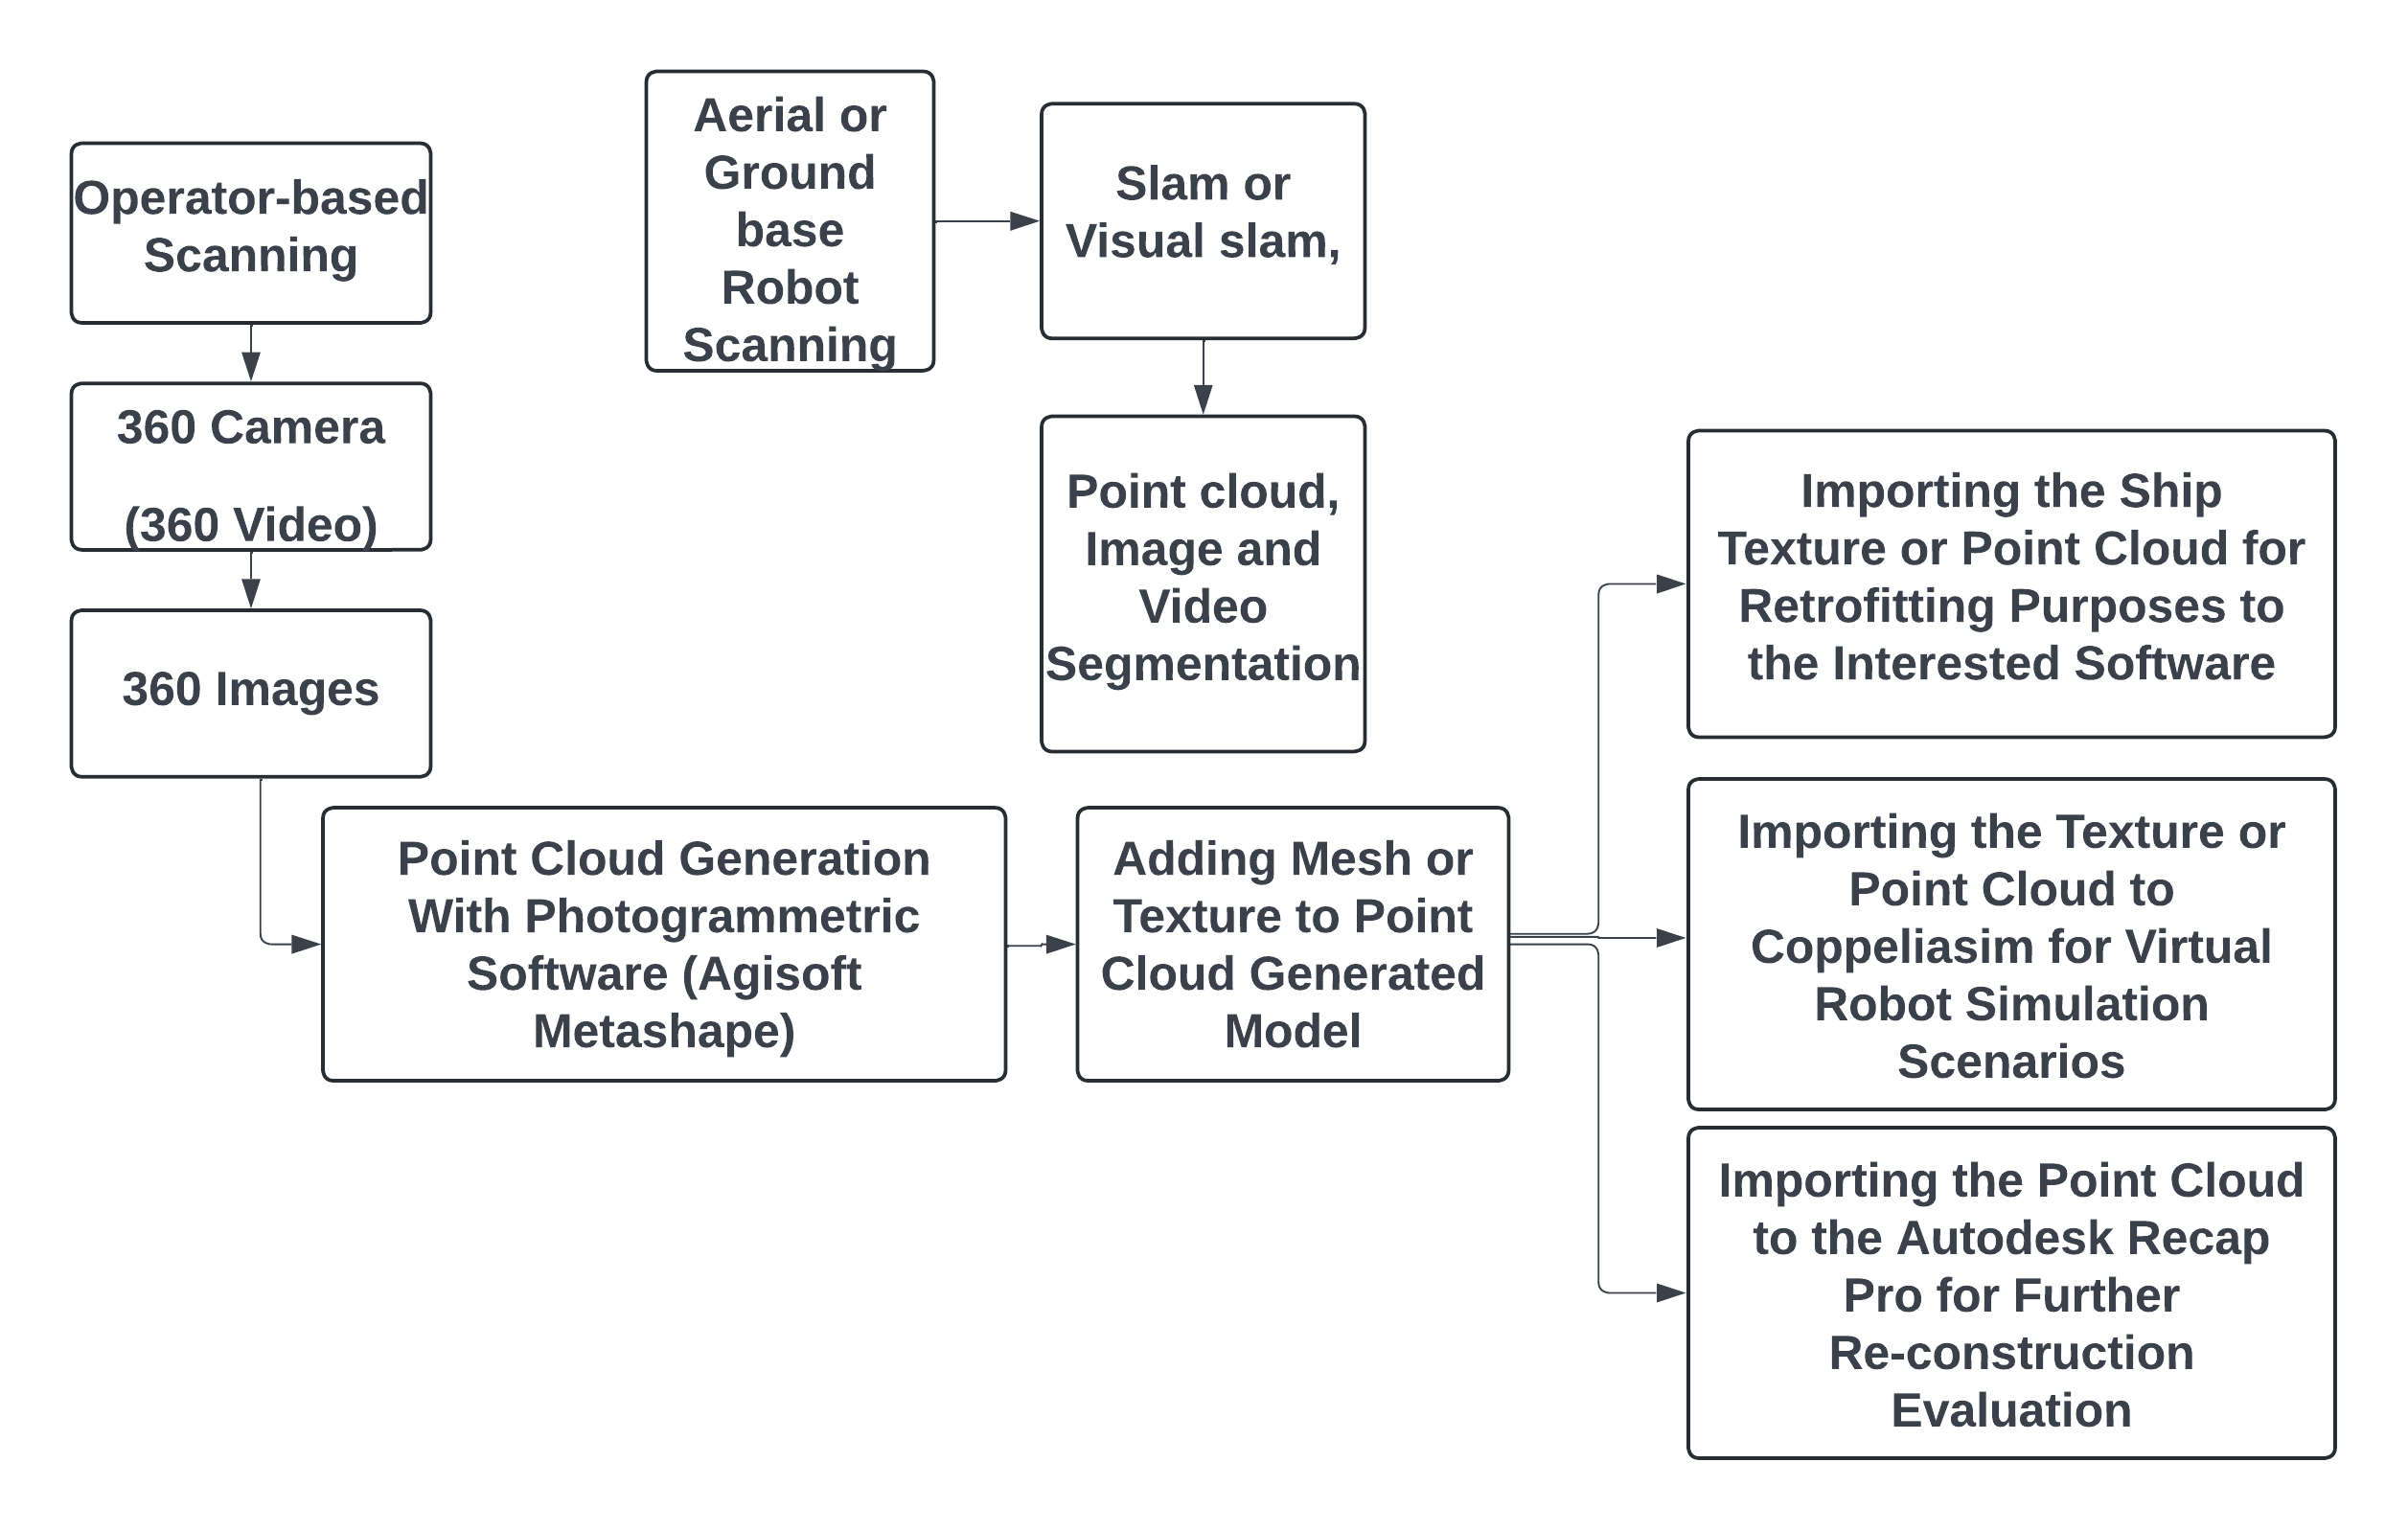
\includegraphics[width= 1.0\textwidth]{Figures/Whole View.png}
  \caption[Holistic View ]{Holistic Flowchart for Human-based and Robot-based Scanning}
  \label{fig:Holistic View}
\end{figure}

\noindent As it is shown in Figure \ref{fig:Holistic View}, two methods planed for this research but just operator-based scanning has been executed in the thesis. And other method concepts (robot-based scanning) mentioned in the literature. Related literature for robot-based scanning (Aerial or Ground) has been explained due to its importance for 3D scanning. 






\section{Project Description}

In this project, I investigate and assess the viability and potential of utilizing operator-based 360$^{\circ}$ scanning technologies for data capturing specifically in the shipbuilding and construction industry then I simulated a robot for fire-fighting scenario in a ship as an outdoor and a hallway as an indoor environment. The work also include some background data on the state-of-the-art scanning techniques and technologies related to shipbuilding industry, and pertinent literature and research on the subjects of neural radiance fields, 360 imaging, photogrammetry, Lidar, and SLAM (for robot-based Scanning).

\subsection{Stakeholders}
A wide range of stakeholders are involved in the discussion of lowering the cost of 3D model re-visioning during ship production and retrofitting in ship life-cycle through innovative technologies. Most of the techniques for 3D scanning and modeling, model-revision during building reconstruction is also applicable. These parties are interested in different aspects of the development, results, and uses of these technologies.\\These are the main parties involved in this situation for ship manufacturing industry. \\

1. Shipbuilding Companies: The main parties who gain directly from lower production costs and increased safety in search and rescue operations and effectiveness in production of the vessels. Technologies that can improve quality, expedite the time to market for new vessels are what they're interested in implementing.\\

2. Ship Owners and Operators: These parties have an interest in how reliable, safe and affordable ships are. Innovations that cut production costs have the potential to minimize vessel acquisition or operating expenses as well.\\

3. Authorities and Safety Organizations:  Organizations that oversee the safety and quality of maritime building. Their area of interest is the impact of emerging technology on adherence to environmental and safety requirements. \\

4. Insurance Companies: companies that offer cargo and ship insurance. They are involved in risk assessment and management since new technologies have the potential to affect the dependability and safety of marine vessels. \\

5. Technology Providers and Innovators: Companies and research institutions that specialize in robotics, LiDAR, photogrammetry, 360 camera systems, and NeRF technologies. They are involved in the research, development, and commercialization of their discoveries.\\

6. Defense Sector: For naval and defense-related shipbuilding, military and defense departments are key stakeholders. They are interested in the strategic advantages and cost savings offered by advanced technologies.\\

\noindent These are the main parties involved for building reconstruction industry.\\

1. Client: Often, the property owner or developer commissions the reconstruction project.\\

2. Structural Engineer: Ensures that the repaired structure is structurally sound and meets safety regulations.\\

3. Contractor:The body responsible for carrying out the reconstruction work in accordance with the project parameters.\\

4. Architect: Plays an important part in designing the reconstruction and ensuring that the new structure fulfills both aesthetic and functional standards.\\

5. Subcontractors: The main contractor hires specialized workers to complete specific jobs such as electrical work, plumbing, and HVAC systems. 

\section{Objective and Research Questions}
Lidar is one of the traditional methods for authentic modelling of buildings for construction purposes. Also use of Lidar in shipbuilding industry for having an accurate 3D model specifically during production and retrofitting is vital. Nowadays with the help of advanced photogrammetry methods, making 3D model is simpler and less expensive than traditional methods. This technology give the equal accessibility to individuals for making 3D models even by a smartphone. After making a 3D model, there are variety of usages for a 3D model, one of them is for simulating a real scenario in a virtual environment like navigating a robot in virtual world that could be at an indoor or inaccessible outdoor location for rescue operations. Another opportunity is adding mesh and texture to the captured point cloud for making a realistic model in retrofitting goals in shipbuilding or construction industry. Due to the lack of industry-applicable resources in operator-based scanning for 3D modeling by 360 degree cameras , I decided to dive into these methods. In this method, an asset scanned and then the video processed with software, and then a point-cloud of that object was made. After visualizing the  point cloud with Agisoft Metashape or other visualizing software it is also possible to make a photo-realistic 3D model of that asset. After adding mesh or even without mesh, 3D model is ready for simulation scenarios, re-construction purposes and ship redesign during production. Mentioned pipeline not only improves the safety and efficiency of marine operations, but it also provides new opportunities for inspection and maintenance chores that were previously difficult owing to the hostile marine environment.  \\

\noindent In this research, we try to address the following questions:\\

\noindent $RQ_1-$ What are the benefits of scanning an object with 360 -degree camera?  \\

\noindent In scanning process I used 360 camera and a software to separate the scanned frames and then stitch the frames or photos together to make a model or point cloud. (Complete answer is in conclusion chapter)



\noindent $RQ_2-$ What are the advantages of using captured point cloud for 3D reconstruction purposes with application in construction industry\\

\noindent After scanning the building, it is possible to import the point cloud to a software and start redesign.(Complete answer is in conclusion chapter)\\

\noindent $RQ_3-$  How to benefit from captured point cloud for more efficient ship maintenance? (This question addressed in literature review)\\
\noindent After scanning of the intended rooms or components in the ship for making a dense point cloud, we can import point cloud on the original CAD model for re-design.(Complete answer is in conclusion chapter) \\ 


\noindent $RQ_4-$ How to investigate the simulation of a robot in a 3D virtual world for safer marine operations?\\
We need a high fidelity virtual environment with real-world physics for this rescue robot to have an interactive and realistic training scenarios. This environment could be a point cloud or a textured model. After importing this model to Coppeliasim robotic simulation software, I fine tuned the robust algorithm parameters for getting optimized result.(Complete answer is in conclusion chapter)    






\cleardoublepage
%the cleardoublepage command ensures that the next text page is on the right-hand side (odd page) and produces a blank page if necessary to achieve that, as all chapters should begin on the right hand side


\chapter{Theory}
%equations, bib. \\

\section{Literature Review}

\noindent This chapter will examine the current literature and research related to different methods of scanning, advantages and disadvantages, weak points and strength of each method. Methods mainly  consists of 360 degree scanning, photogrametry, Lidar with a sample used case for ship damage assessment, NeRF and 3D Gaussian Splatting for scanning and photo-realistic 3D models. For Aerial-based or ground-based robot scanning equipped with 360 degree camera, concepts of slam and visual slam is crucial which mentioned in this study for further work and not as a used case in my methodology. Final section of this chapter is about variety of segmentation methods for image, video and point cloud which is important specially for robot-based scanning. 
\subsection{Shipbuilding processes related to 2D and 3D modeling}
The development of large and complicated products such as ships, ferries, and offshore boats is a lengthy process that encompasses all activities till product delivery (conceptual design phase, construction and assembly phase, etc.).  Life cycle management is a difficult challenge for maritime transportation vehicles, which have long lifespans (more than 15 to 20 years) and a variety of operational conditions \cite{Favi2018}. \\ An overview of shipbuilding processes which related to 2D and 3D modeling of a ship: \\
\textbf{1. Conceptual Design:}  This phase consists of the initial ideation and drawing of the ship's design, with an emphasis on its intended purpose, capabilities, and overall attributes. In this phase possible to define the vessel's general characteristics and measurements, as well as outline requirements. For this phase designer company could develop precise general arrangement drawings, reuse current designs and previously created projects, make diagrams, and pinpoint the major equipment \cite{Favi2018}.\\
\textbf{2. Basic Design:} This phase involves comprehensive planning and design refinement, as well as detailed drawings and specifications \cite{Favi2018}. The basic design incorporates the hull form, general arrangements, needs, and other information from the initial design to create a fully working vessel. This encompasses an initial design of the structure for all crucial sections, a comprehensive analysis of the structure, designs for functional machinery and systems, space distribution for key systems, preliminary lists and specifications of equipment, models for estimating weight, and drawings approved by the class.”. To meet the industry's stringent design timetables, all team members must collaborate, from structural designers to those in charge of assigning space for critical systems. When everyone understands the implications of a change, it is simple to respond before problems occur. It also informs the entire team about progress, other essential elements such as weight management, and both intra and inter-disciplinary conflicts in the project\cite{Thedesignphase}.\\
\textbf{3. Detailed Design :}
In-depth engineering effort to complete the ship's design for construction. Even before the basic design's class approval package is granted, work is underway to add the detail required to source material, plan the construction, and drive fabrication and assembly of the vessel in the yard. This effort marks the start of the comprehensive design and will continue until the vessel is completed and ready for launch. It is crucial that this work represents a natural extension of the original idea. It is also critical that the engineering team respond promptly and efficiently to change requests, whether they come from class society comments if the basic design has not yet been authorized, production concerns, or unforeseen changes in equipment or material \cite{Thedesignphase}.\\
\textbf{4. Manufacturing and Assembly :}
Even a little shipbuilding project is massive in scope and size. Structural parts are manufactured, and interim assemblies are created specifically for that series of ships. Even within two ships in the same series, there are more differences than similarities.
For these reasons, a shipyard's deliverables are numerous, complicated, and unique to shipbuilding. The organization's design and engineering teams must be able to provide these shipbuilding deliverables while also dealing with shipbuilder-specific problems\cite{Thebuildphase}. \\
\textbf{5. Digital Twin, Maintenance and Retrofitting :}
While shipbuilding can take years, a ship will be in operation for decades, and expense distribution is the same. Even a little reduction in a ship's long-term expenditures can result in enormously huge savings when compounded over its lifetime. When the ship is turned over to the client, the digital information must stay associated with it. However, if digital data is not available, your teams must be able to gradually develop the digital twin after the event. Using technology such as laser scanning or other data collection methods to capture the vessel's on-the-water status and integrating it with any CAD, PDF, or other available data can provide your business with a comprehensive picture of the ship. Integrating data from multiple sources helps capture the intent underlying digital information and maintains the digital thread. The result is a higher ROI (Return on Invest) for boats with better-managed data. When stricter environmental standards meet longer vessel lifespans, hundreds of ships require retrofitting, maintenance, or both. Making that process as frictionless as possible, with minimal downtime, is critical to minimize the impact on a business. Every retrofit process begins with an assessment of the ship's current condition. If the ship's digital twin has not been updated throughout its career, or if the ship was built without one, the retrofit designer will most likely be unable to use existing data. This means starting from scratch but the goal is to find the most cost-effective, scalable, and efficient method of collecting on-board reality and developing adjustments without losing quality. Each retrofit project presenting unique issues and each vessel differing somewhat, using laser scanning is one method to guarantee you have as much information as possible to assist you throughout the design process \cite{LaserscanSSI,Stavroulakis2022}.

\subsection{The Role of 3D Scanning in Ship's Safety and Maintenance}
The efficiency of a ship's machinery, especially the plumbing in the engine room, is critical to its functioning and safety. The maritime sector is significantly reliant on this machinery, which affects not only the crew's lives but also the sea environment. 3D scanning technology contributes significantly to the maintenance of these systems by:\\

\textbf{1. Accurate Model Creation :} It generates comprehensive models of the engine room's pipework, allowing you to pinpoint parts that are likely to fail.\\

\textbf{2. Support of Maintenance :} The 3D models are useful references for doing inspections, repairs, and managing complex installations or retrofits.\\

\noindent 3D scan of different components in the ship can be used for inspection, reference for repairs or retrofits and complicated installation. The scanner can generate the raw data or point cloud and in the next step the technicians can make a CAD model of that components \cite{3DScan}. In Figure \ref{fig:Engine Room Scan} there are scans of engine room of a ship. 


\begin{figure}[H]
  \centering
  \subfloat[Engine Room scan in a ship]{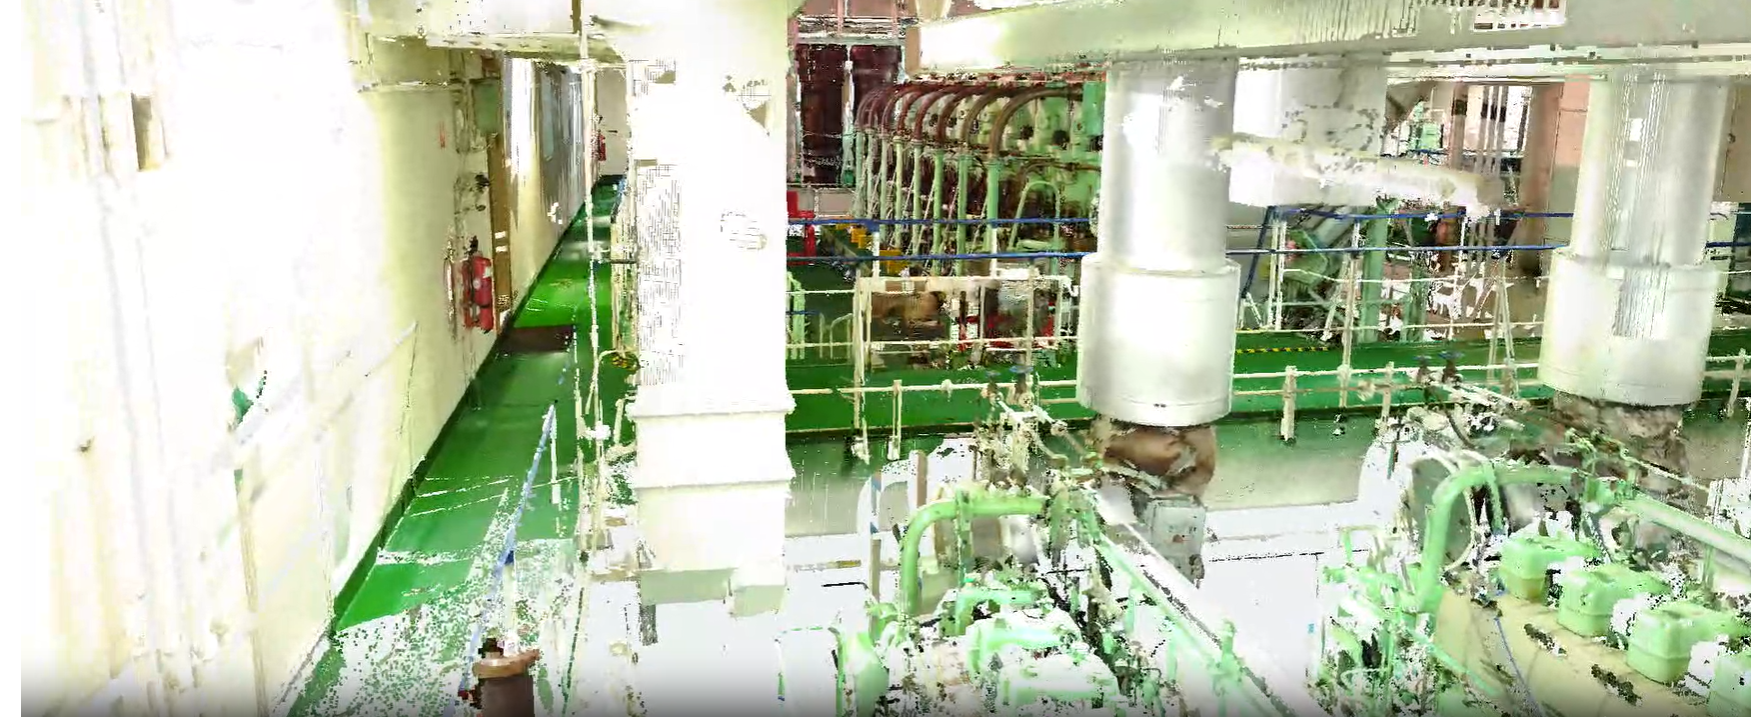
\includegraphics[width=0.9\textwidth]{Figures/EN2.png}\label{fig:Engine Room Scan}}
  \hfill
  \subfloat[Engine Room Scan 2]{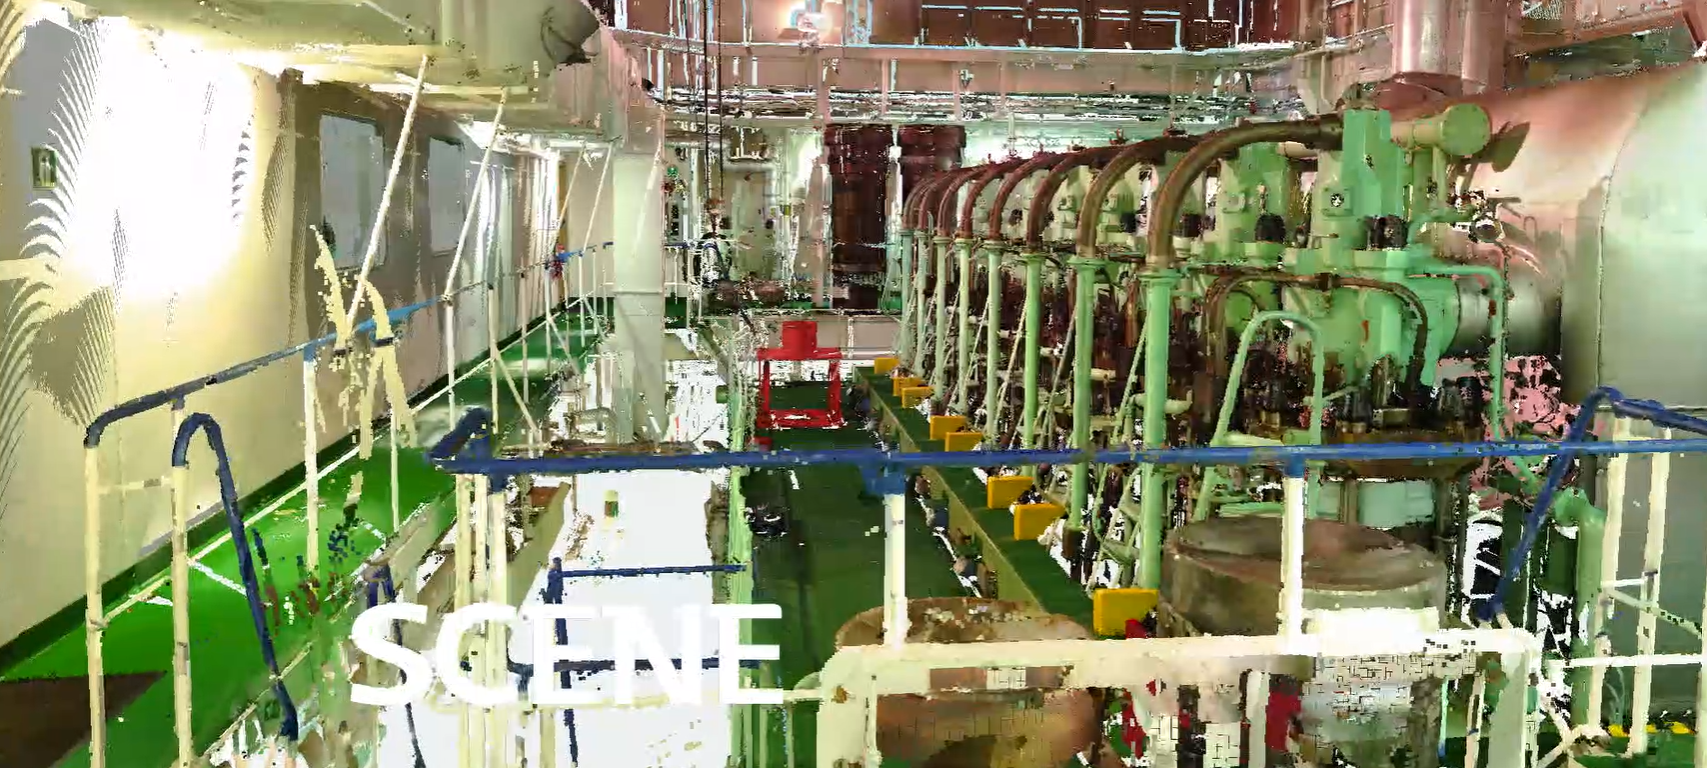
\includegraphics[width=0.9\textwidth]{Figures/ER3.png}\label{fig:Engine Room Scan 2}}
  \hfill
  \subfloat[Engine Room Scan 3]{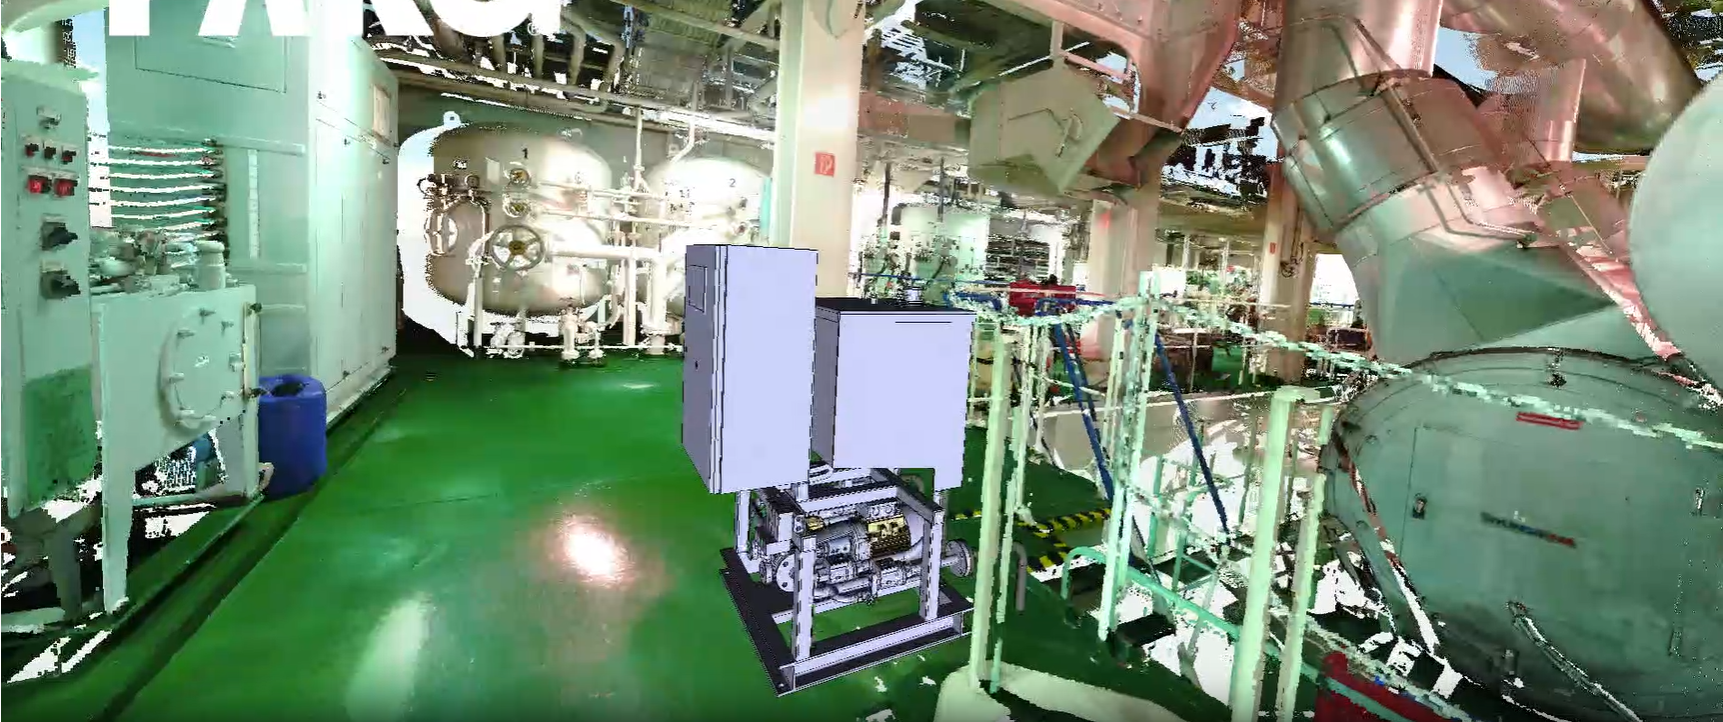
\includegraphics[width=0.8\textwidth]{Figures/ER5.png}\label{fig:Engine Room Scan 3}}
  
  \caption[Engine Room Scans from Different Views]{Figure (a) shows the point cloud from engine and pipes, figure (b) shows another view of scan in engine room, and figure (c) shows components point cloud.}
\label{fig:Engine Room scan in a Ship} \cite{3DScan}
\end{figure}

\subsubsection{Integration of Scanned Data Into the Design}
Scans of individual fabrications, modules, or as-built sites can be quickly imported and verified against the design model. 
Keep your project on track by identifying and resolving non-compliances. Use a design model that can be updated to correctly reflect the actual construction \cite{AVEVAE3D}. In the Figure \ref{fig:Laser data merge with 3D} it is shown that laser scanned equipment data are integrated with green pipes from the original 3D CAD model. 

\begin{figure}[H]
  \centering
  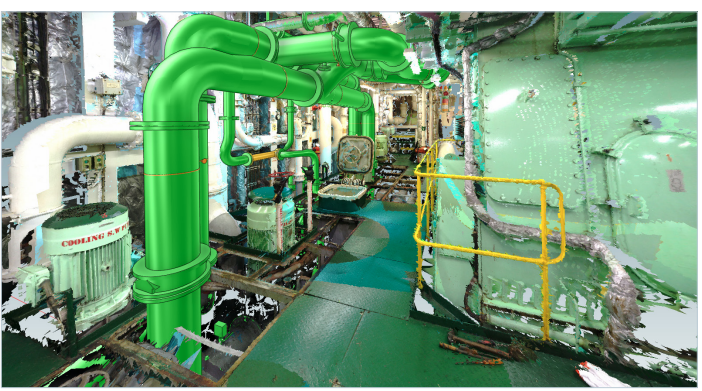
\includegraphics[width=0.9\textwidth]{Figures/AVEVAE3D.PNG}
  \caption[laser data integrated with 3D CAD model in AVEVA E3D software]{Laser scanned data merged with 3D model} \cite{AVEVAE3D}
  \label{fig:Laser data merge with 3D}
\end{figure}

\subsection{360$^{\circ}$ Camera Systems}
 This sub-chapter delves into how these 360$^{\circ}$ camera systems are used to conduct a comprehensive and complete environmental evaluation, which is critical for the planning, construction, maintenance, and operation phases of shipbuilding and maritime activities. This part attempts to provide light on the mechanics, uses, and benefits of 360$^{\circ}$ camera systems, as well as their role in improving operational efficiency, safety, and cost-effectiveness in maritime situations.
Omnidirectional cameras, often known as 360 degree cameras, capture images and videos with a full spherical view. Because of its ability to record immersive and interactive information for virtual reality. 
These cameras are increasingly used for augmented reality and multimedia applications. 360 degree cameras are currently used in industries such as real estate, tourism, and entertainment, but the technology's potential extends far beyond these.Advancements in image and video quality, the incorporation of AI and machine learning, and the increasing availability of software and platforms for making, editing, and sharing 360-degree content have led to a surge in its popularity. The future of 360-degree cameras is promising. Despite the expansion, obstacles remain, including high production costs, lack of standardization, and the need for improved software. 360 degree cameras differ not only in hardware and software, but also in crucial aspects that set them apart from each other. These include resolution. This determines the level of detail obtained in an image. Frame rate refers to the number of frames per second collected in a video. The ISO range determines a camera's sensitivity to light
 \cite{karkhanis2023complete}.

\subsubsection{Performance}
A 360 degree camera uses multiple lenses or a single fisheye lens to record a complete spherical image from all angles. 
The camera then uses software to stitch the images together, creating a 
smooth, panoramic image. These photographs can be viewed on a computer or with virtual reality headsets, providing a 360-degree view of the area. 360 degree cameras may capture 360-degree video, enabling immersive experiences for virtual tours and interactive content \cite{Thebest360camerasin2024}.
   
\begin{figure}[H]
  \centering
  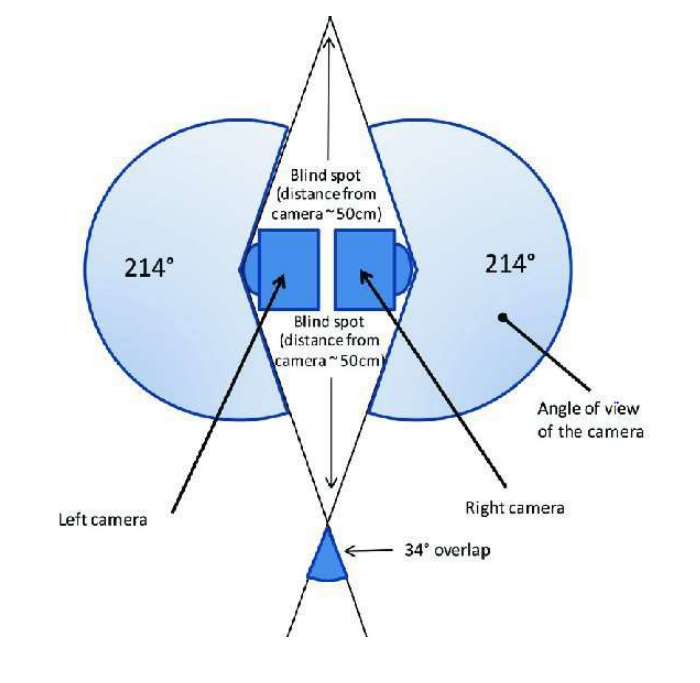
\includegraphics[width=0.9\textwidth]{Figures/360 camera coverage.PNG}
  \caption[Illustration of two camera 360 coverage]{Illustration of two camera 360 and their coverage around} \cite{karkhanis2023complete}
  \label{fig:360 camera coverage}
\end{figure}

\subsubsection{Advantages of 360 cameras}
There are several advantages to using 360-degree cameras, including:  \\
1. Immersive feeling: 360-degree cameras offer a totally spherical image, allowing viewers to see the entire scene from any angle. As a result, the viewer gets an immersive experience. This gives people the impression that they are physically present. \\
2. All-around: 360-degree cameras have numerous applications, including real estate, tourism, events, and personal use. They are useful for creating interactive video content, virtual tours, and other applications. \\
3. Expansion field of vision: A conventional camera's field of vision is limited by its lens. A 360-degree camera can capture the entire environment, providing a far wider field of view. \\
4. Virtual Reality: As virtual reality becomes more popular, 360-degree cameras are being employed to create videos on the platform. The use of 360-degree cameras greatly enhances the immersive VR experience \cite{karkhanis2023complete}. \\
\subsubsection{Constraints} 
\noindent 1. Quality: The camera's resolution, frame rate, and ISO range impact the quality of 360-degree images and videos. Lower-quality cameras may create photos or movies with reduced detail and motion blur. \\

\noindent 2. Stitching: Creating a seamless panoramic image requires stitching together several photographs or video frames. This method is time-consuming and may result in noticeable stitching flaws or inconsistencies in the final image. \\

\noindent 3. Lighting: Capturing photographs or films with a 360-degree camera can be challenging due to lighting. The camera captures light from all angles, which might cause uneven lighting or glare. \\

\noindent 4. Camera Swing: 360-degree cameras can suffer from camera wobble and motion blur due to their tiny size and lightweight design. \\

\noindent 5. Post-Production processing:Editing and post-production for 360-degree videos and photos can be time-consuming and expensive due to the need for specific software and skills. In recent advanced and newer consumer cameras, the problem of stitching and time-consumption has been substantially reduced.   \\

\noindent 6. Privacy: Capturing photographs or movies using a 360-degree camera might pose privacy problems as it captures a large field of view, potentially including individuals or private property without consent \cite{karkhanis2023complete}. But in industrial used case this item is not a consern. 



\subsection{Photogrammetry using a DSLR Camera or Smartphone}

\noindent Photogrammetry is a photographic technique that produces 3D data (measurements) from 2D images (photographs), resulting in a variety of end-results, first being a point-cloud, second is a depth map and then a mesh and finally a textured model of the object or environment with realistic color. Three main software are Metashape, Meshlab and reality-capture, by using these software you end up with a digital 3D asset.   Basically, you take a series of pictures of an object from various angles, run them through a computer application called Metashape, and you end up with a digital 3D asset. Because light and imaging methodology is so important in this process, certain objects are difficult to capture, if not impossible, to model using photogrammetry: objects with reflective or shiny surfaces, clear/transparent objects like glass, very thin objects like tree leaves, very furry or hairy things, and moving objects may sufer from these parameters\cite{PhotogrammetryWorkflowusingaDSLRCamera}.

\noindent Photogrammetry and laser scanners are now commonly used to document 3D models. Research indicates that laser scanners produce geometric data such as point-cloud and textured meshes, but photogrammetry produces higher resolution textured meshes. The high cost of laser scanners has hampered documentation practices, particularly for institutions and individuals with low means. This promotes digital photogrammetry with DSLR cameras as standard instruments although these processes are also quite time-consuming and expensive in the capture of outdoor assets or environments under sunny conditions, this also presents a set of problems due to the time takes to capture the environment or asset or the movement of the sun.Making it favourable to do such capture when it is overcast. In sunny weather , the asset or the environment tend to reflect the sun light as well as shadows which again will move due to the movement of the sun. Digital camera technology has advanced to the point where smartphones now include cameras\cite{samosir2020comparison}. \\ Smartphones are increasingly being used in photogrammetry. Smartphones are mostly used for 3D modeling because of their computer power and user-friendly software, being a cheaper alternative compare to specialized equipment such as DSLR cameras and laser scanners. Some smart phone also have integrated lidar modules. Smartphones are mostly used for rapid scanning of environments and smaller objects, enabling to capture a point-cloud and create a 3D mesh but due to inferior sensor size and lens quality the texture will suffer from less quality and resolution. \cite{Jasińska2023}. 


\begin{figure}[H]
  \centering
  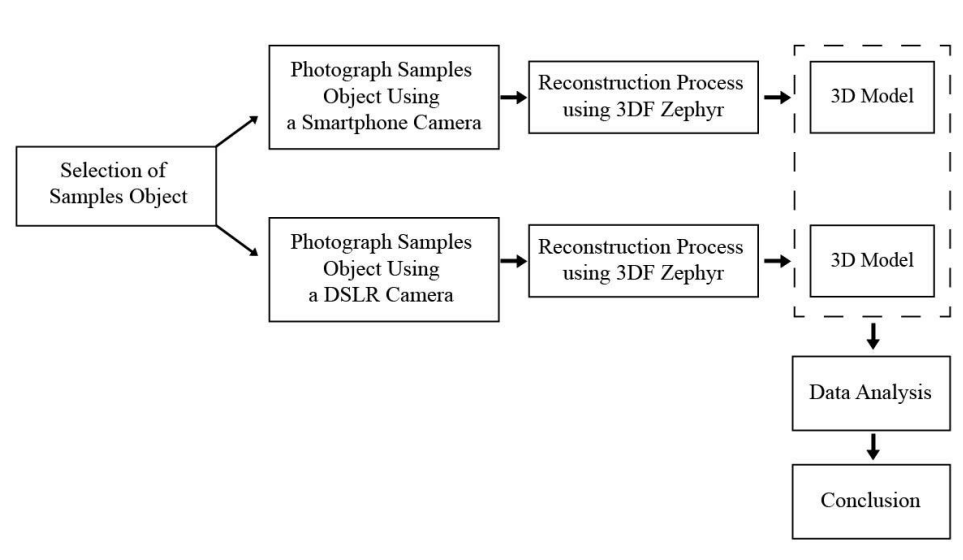
\includegraphics[width=1.01\textwidth]{Figures/Photogrammetry with DSLR Camera and Smartphone.PNG}
  \caption[Workflow of photogrammetry with DSLR camera and smartphone]{Workflow of photogrammetry with DSLR camera and smartphone} \cite{samosir2020comparison}
  \label{fig:photogrammetry with DSLR camera and smartphone}
\end{figure}

\subsection{Lidar}
Recently, the application of Light Detection and Ranging (LiDAR) technology has become widespread in various fields. The LiDAR system design has greatly improved over the years, resulting in a design that is incredibly low in cost, size, weight, and power (SWaP). Because LiDAR is lightweight and energy efficient, its use in aerial and mobile platforms has grown to allow mapping and obstacle avoidance, both of which were previously thought to be difficult. The classification of LiDAR equipment can be broad and subjective, depending on the context of use. Nonetheless, this instrument is generally classed based on the three types of information-capture functions it provides: spatial, spectral, and temporal. Every LiDAR equipment requires the ability to capture spatial information.This information is often gathered by time of flight (TOF) measurements. LiDAR systems capable of gathering spatial information are available in three varieties: one-dimensional (1D), two-dimensional (2D), and three-dimensional (3D), with optical deflecting systems used to collect 2D and 3D spatial information, respectively. The spatial data is required for creating an accurate 3D map of the environment. Creating an accurate 3D map of the environment necessitates spatial data. Yet, for applications requiring object detection, geographical information on its own is inadequate. The second class of LiDAR sensors may measure spectral information about a substance, such as laser return intensity (LRI). The term LRI refers to the reflectance caused by the interaction of the wavelength of the transmitted pulse from the LiDAR device with the targeted substance.Because the LRI is unique to a particular material type, it may be useful for determining the surface attributes of a target material. However, to avoid ambiguity in LRI readings, at least two laser wavelengths are required. Furthermore, some applications demand temporal information gathering capabilities in addition to spatial and spectral information. This can be accomplished by employing the repeated LiDAR approach\cite{raj2020survey}. Repeated LiDAR is the process of collecting temporal data from a target environment over a set length of time \cite{robin2014making}. Temporal data is critical for understanding dynamic processes like plant development and soil erosion \cite{eitel2016beyond}.\\
\subsubsection{LiDAR Architecture}
\noindent The LiDAR architecture is explained as the art of LiDAR instrumentation concerning LiDAR hardware and software \cite{FundamentalsofLidarRemoteSensing, PhysicalPictureofLidarEquation}.
A completely functional LiDAR system consists of four key subsystems: laser rangefinder, beam deflection, power management, and master controller units, as shown in Figure \ref{fig:Block diagram of LiDAR}. 
Each of these fundamental blocks is equally essential, and a malfunction in any of these subsystems could lead to a decrease in the LiDAR system’s functionality. However, without the beam deflection subsystem, the LiDAR might still work as a 1D LiDAR, also known as a laser range finder (LRF)\cite{raj2020survey}.

\begin{figure}[H]
  \centering
  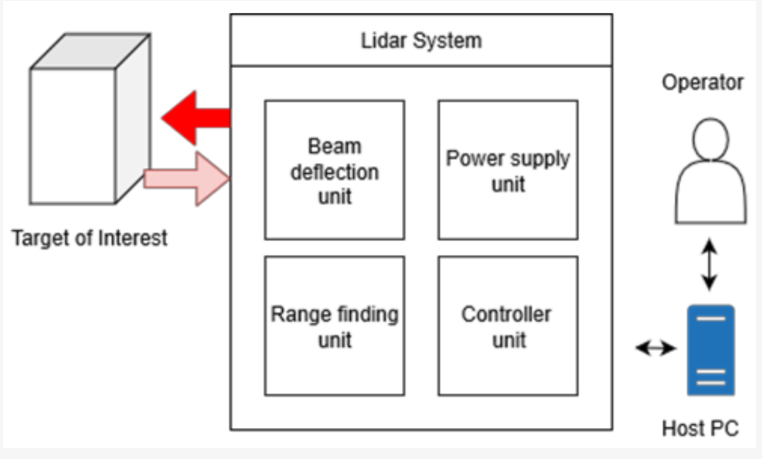
\includegraphics[width=0.9\textwidth]{Figures/Block diagram of LiDAR system.PNG}
  \caption[Illustration Block diagram of LiDAR]{Illustration of Block diagram of LiDAR} \cite{raj2020survey}
  \label{fig:Block diagram of LiDAR}
\end{figure}

\subsubsection{LiDAR Specifications}
The LiDAR scanner parameters are critical information for a developer to select the best solution for his application. It can be divided down into four tiers, as shown in Figure \ref{fig:Hierarchy of LiDAR specifications}. 
The first parameters in the hierarchy include information about ranging, such as maximum and minimum detection range, resolution, accuracy, and update frequency. The second specification in the hierarchy is connected to physical aspects such as size, weight, and power consumption, which can be found in a product manual. These criteria are critical for applications involving mobile or aerial platforms where size, weight, and power may be limited. Because LiDAR uses lasers, information about the wavelength, power emitted, and laser class is provided in the specs to ensure safety compliance.Examples of optical specifications mentioned in product manuals include lens focal length and beam divergence. The specs provided thus far only define the properties of 1D LIDAR. In the case of scanning LiDAR, extra parameters about beam deflection motion are required. This specification defines characteristics such as field of vision (FOV), angular resolution, response time, and number of scan points \cite{raj2020survey}.
\begin{figure}[H]
  \centering
  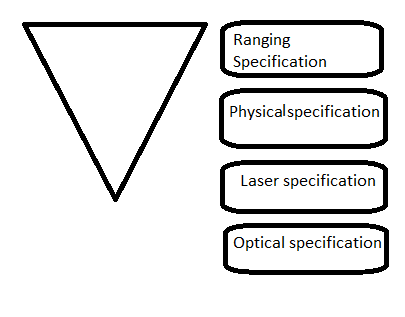
\includegraphics[width=0.8\textwidth]{Figures/Hierarchy of LiDAR specifications.png}
  \caption[Illustration of Hierarchy of LiDAR specifications]{Illustration of Hierarchy of LiDAR specifications} \cite{raj2020survey}
  \label{fig:Hierarchy of LiDAR specifications}
\end{figure}
\subsubsection{Used Case of LiDAR and 3D Ship Model for Battle Damage Assessment in a Frigate}


The static detonation training exercise in late March 2022, during which an explosive charge was placed aboard the ship with the intention of harming it, and the future evolution are essential components of a lidar-focused megaproject financed by the Naval Innovative Science and Engineering (NISE) program. As part of the project, different combat centers collaborate to create 3D models of complete ships from lidar scans, with the goal of expanding the models' use in battle damage assessment and repair, installation and modernization, and other fleet applications \cite{defenseadvancement}. \\
This technology allows for the speedy capture of damage, overlaying it on the baseline model, precisely documenting the state, and then sharing the data with the greater community to help engineers make decisions. The initiative comes as lidar scanning tools become more accessible and affordable. By leveraging technology to create more 3D ship models, stakeholders and partners hope to reduce the need for engineering teams to travel to ships, enable more remote support such as virtual ship checks, and reduce response times to casualties and maintenance issues that the fleet encounters at sea. Because it is possible to send the 3D model to the people but not the ship. Lidar examines an object in three dimensions by bouncing laser beams off of it and timing how long they take to return. The system can record a massive network, or cloud, of data points and stitch together scans from various angles to produce a millimeter-accurate 3D digital image of the object \cite{LidarSolutionforship, deems2013lidar}. The most recent lidar scanning equipment can also collect images and overlay them on the data point cloud, resulting in a more realistic model. \\
More accurate installation drawings, for example, could aid in the avoidance of unexpected hurdles and delays during ship construction. Lidar scans can generate 3D models of ships that are precise to the millimeter. Installation and upgrade teams can use these models to measure parts of the ship before embarking to install equipment. In this digital environment, it is feasible to collect exact measurements between components as well as calculate distances between bulkheads and equipment. Designers can ensure that doors and cabinets open properly.  Engineers are looking for obstacles to our installation that need to be moved or planned around. Due to high expenses of this method, it is better to involve interested-parties who works on different areas of a ship \cite{defenseadvancement}. 
\subsubsection{Full Ship Scan}
In 2020, the complete interior and exterior of the amphibious transport dock USS San Diego (LPD 22) were lidar-scanned. The end result was the first full-size 3D digital model of an LPD-class vessel. Scanning a complete ship may appear expensive due to the massive data collection and processing required. Approximately the course of roughly two months, the team that scanned the USS San Diego collected approximately 7,000 unique scans from various points within and outside of the mammoth warship. Full-ship scanning gains even more value when its application spreads across other fighting centers. In other words, the cost per user decreases as the number of stakeholders using the data collection increases\cite{defenseadvancement}. 
\subsubsection{Combination of Photogrammetry and LiDAR in Ship Damage Assessment}
Ships can sustain various sorts of damage, including structural damage from weapons attacks, collisions, corrosion \cite{aijazi2016detecting}, and exceeding operational loads. Normally, damage assessment inspectors must visit to the ship to assess the damage, take photos, and write a report. To respond to casualties more efficiently and precisely, Nahshon realized the potential of comparing a ship's "healthy" pre-casualty 3D model to its damaged condition. Unmanned aircraft systems (UAS), commonly known as drones, make it easier to acquire photographs and videos of damaged regions aboard ships. Photogrammetry, a sort of 3D scanning, involves stitching together footage from a UAS to create a 3D depiction of the damaged region. This updated model might then be compared to the lidar scan's pre-casualty healthy model to get a more accurate picture of the damage \cite{defenseadvancement}. 

\subsection{Preface for Simultaneous Localization and Mapping (SLAM)}
SLAM, or simultaneous localization and mapping, is a subject in mobile robotics and artificial intelligence that has been extensively studied for over two decades. Scientists employ many approaches to enhance the autonomy and self-exploration of robot navigation. Autonomous robots are intelligent systems that can navigate their surroundings without human intervention. To navigate successfully, robots must have a strong grasp of their surroundings and accurately track their whereabouts.The robot's location, also known as its state, determines its pose, position, and orientation on the map. The map depicts the environment's elements, such as walls, barriers, and landmarks. A map is necessary for mobile robots to navigate and plan their paths. Localization refers to the process of predicting a robot's position in recognized environments using sensor data and a pre-defined map \cite{thrun2002probabilistic}. 
Numerous studies have examined the localization problem across various criteria and situations. A fully intelligent mobile robot should be able to explore unfamiliar environments without relying on a pre-existing map.For indoor applications where GPS is not available, a reliable mechanism for estimating the robot's stance is necessary.However, the popularity of applications that erase user-created maps has made mapping necessary for mobile robots. The SLAM technique is effective for solving problems when prior knowledge or maps are unavailable or undesirable. SLAM techniques create a map of the environment without prior information and locate the robot without human input. It allows robots to operate without relying on ad-hoc localization infrastructure. Robots require a map (e.g., identifiable landmarks) to rectify misalignments caused by uncertainties in their movements, such as drifts and dead reckoning.Future SLAM systems should provide autonomous navigation in all environments, including indoors, outdoors, underwater, and air, with minimal estimation errors, long-lasting mapping, and low-power and computing costs. Simplicity is also important \cite{Taheri2021}. 
\subsubsection{Simultaneous Localization and Mapping (SLAM)}
SLAM solution strategies have advanced rapidly over the last two decades. SLAM algorithms utilize numerous sensors, including ultrasonic sensors, laser scanners, and RGB cameras, to estimate robot stance and create two- or three-dimensional maps. The 2D SLAM challenge with rangefinders is considered solved \cite{li2016real}, however, this assertion is incorrect, as advances in accuracy, speed, and massive data processing are needed for 2-D SLAM problems. Unmanned systems, including UAVs, self-driving cars, building inspections, surveillance, and underwater SLAM, face challenges in outdoor, unstable, and dynamic environments. Furthermore, every technique has room for improvement. Most SLAM failures are caused by perception instability or uncertainty. SLAM includes two parts: localization and mapping. Initially, SLAM technology focused on mapping and localization individually. Modern studies recognized that localization and mapping are very interdependent. The map is necessary for accurate localization, whereas localization is crucial for mapping. As a result, the word is known as a ''Chicken and egg'' question. Classical SLAM algorithms estimate poses and maps collaboratively. However, more sophisticated systems view localization and mapping as two simultaneous operations, resulting in the well-known simultaneous Tracking and Mapping (PTAM) \cite{klein2007parallel,Taheri2021}. 
In robotics, odometry is the estimation of a robot's motion over time using motion sensors such as wheel encoders. Odometry models using various sensors, including Visual Odometry (VO) with cameras, have advanced significantly. Improving the precision of the odometry model reduces uncertainty in robot navigation and improves mapping. Mapping is significant in three fundamental aspects: \\
1. Maps provide path planning and obstacle avoidance. \\
2. Many mobile robotics applications aim to create maps.\\
3. The durability and accuracy of localization are highly dependent on mapping accuracy.\\
Loop closure is a key component of mapping, allowing robots to recognize visited locations and optimize their estimated poses. The loop closure significantly decreases drifts and allows the robot to adjust for odometry inaccuracies. Visual odometry approaches often incorporate mapping, but the map may not be relevant to path planning or local task execution. SLAM varies from modern odometry models by optimizing the global map and closing the loop \cite{cadena2016past}. Positioning is an important aspect of SLAM. There are two approaches to tackling positioning difficulties: probabilistic and non-probabilistic. Probabilistic approaches are often used for categorization. Probability approaches rely on Bayesian estimates, primarily using Particle Filters (PF) and Kalman Filters (KF). Gaussian distributions are used for system inputs, motion model output, observed data, observation outputs, and state noise. KF provides the most accurate assessment of the robot pose \cite{yavuz2009simultaneous}.
The KF-based SLAM approach is popular due to its simplicity of implementation and advantage in convergence. However, it lacks a loop closure and has issues with data association, which can lead to system failure. KF is typically applied to linear systems, while nonlinear systems are more common in practice. Nonlinear systems can be linearized with the Extended Kalman Filter (EKF) and first-order Taylor expansion \cite{julier2001counter}.\\
An overview of a standard SLAM algorithm based on the EKF is provided below: \cite{Taheri2021}\\
\noindent 1. The elementary map is created using initial sensory input.\\
2. Characterizes the robot's beginning stance and surrounding locations.\\
3. The robot updates its location and map information as it moves around.\\
4. New landmarks are derived from the revised map.\\
5. The robot recognizes new landmarks and adjusts its location accordingly.\\
6. The robot follows a new path based on the updated map until it reaches its destination.\\
 Figure \ref{fig:Feature based slam} depicts a common block diagram for a feature-based SLAM issue \cite{leonard2012directed}. 
\begin{figure}[H]
  \centering
  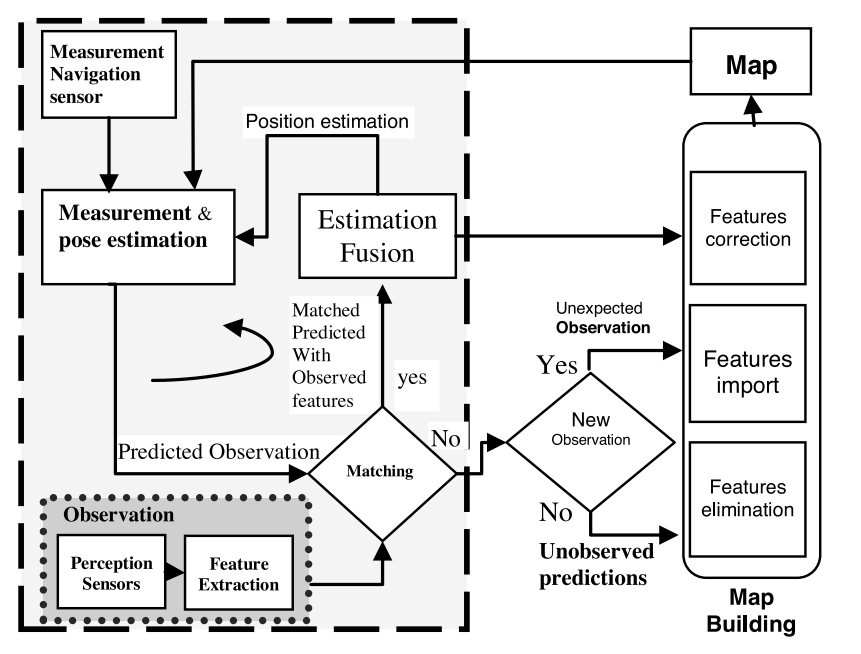
\includegraphics[width=0.9\textwidth]{Figures/Feature based slam.PNG}
  \caption[Illustration of Feature based slam]{Illustration of Feature based slam} \cite{leonard2012directed}
  \label{fig:Feature based slam}
\end{figure}

\subsection{Visual SLAM}
Simultaneous Localization and Mapping (SLAM) captures the 3D structure of an unfamiliar environment while also tracking sensor mobility. This technique was initially presented for autonomous control of robots in robotics \cite{chatila1985position}. SLAM-based applications have expanded to include computer vision, online 3D modeling, AR visualization, and self-driving cars \cite{durrant2006simultaneous,bailey2006simultaneous, stachniss2016simultaneous,aulinas2008slam}. In this section, we talked about  SLAM employing cameras due to their simple sensor design and higher technological hurdles compared to other methods. Visual SLAM (vSLAM) is a technology that relies solely on visual information as input. vSLAM algorithms have been widely used in computer vision, robotics, and augmented reality \cite{billinghurst2015survey}. These methods are ideal for estimating camera poses in AR systems with simple configurations, such as camera-mounted tablets or smartphones. Real-time response is a key requirement in AR systems because it allows real and virtual items to be smoothly and interactively merged.The use of vSLAM algorithms is not limited to AR systems. It has applications in robotics, such as unmanned autonomous vehicles (UAVs). In general, vSLAM is more technically challenging than other sensor-based SLAMs since cameras can capture less visual information from a smaller field of view than 360° laser sensing, which is commonly employed in robotics. Camera postures must be continuously calculated from such data, while the 3D structure of an unknown environment is recreated at the same time. In the 2000s, the early work on vSLAM with a monocular camera focused on tracking and mapping feature points. This is referred to as "feature-based approach." To deal with texture-less or feature-less surroundings, vSLAM has been developed that works without detecting feature points and instead tracks and maps the entire image. This is known as "direct approach". With the introduction of low-cost RGB-D sensors such as the Microsoft Kinect, vSLAM algorithms that use both a monocular picture and its depth have been developed  \cite{Taketomi2017}. 
\begin{figure}[H]
  \centering
  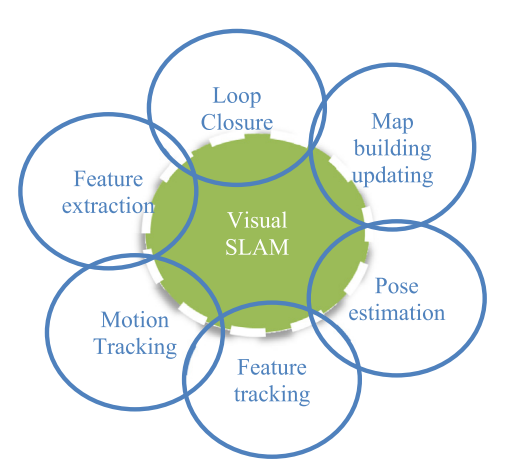
\includegraphics[width=0.6\textwidth]{Figures/Visual SLAM Components.PNG}
  \caption[Illustration of Visual SLAM Components]{Illustration of Visual SLAM Components} \cite{Taheri2021}
  \label{fig:Visual SLAM Components}
\end{figure}


\subsection{Neural Radiance Field (NeRF)}
Synthesizing new viewpoints on a scene from a small number of gathered photographs is a long-standing computer vision problem that is necessary for many AR and VR applications.
Classic techniques, such as structure-from-motion or image-based rendering, have been employed to tackle this problem 
 \cite{martin2021nerf,shum2008image}. Neural rendering techniques, which incorporate learning modules into a 3D geometric context and train them to rebuild observed images, have led to tremendous development in this discipline. The Neural Radiance Fields (NeRF) technique uses neural network weights to model a scene's radiance and density \cite{mildenhall2021nerf}.
 View synthesis involves creating fresh perspectives of a scene using input photos and camera poses. Accurately handling complicated geometry and material reflectance attributes is crucial for creating lifelike outputs from different perspectives. 
Several scene modeling and rendering solutions have been proposed to address this issue, but none have yet achieved photorealistic quality across a large camera baseline \cite{mildenhall2021nerf}.
NeRF is only effective in controlled conditions where the scene is taken quickly with continuous illumination and static material. Moving objects or varying illumination severely reduce NeRF's performance, as demonstrated \cite{martin2021nerf}. Mildenhall and his group provides a cutting-edge strategy for creating innovative views of complicated scenes by maximizing a continuous volumetric scene function using sparse input views. Their algorithm uses a nonconvolutional deep network to represent a scene. It takes a single continuous 5D coordinate (x, y, z) and viewing direction  \(\theta,\phi\)\ as input and outputs volume density and view-dependent radiance. They create views by querying 5D coordinates along camera rays and use volume rendering algorithms to project colors and densities into a picture. Volume rendering is naturally differentiable, therefore optimizing the representation requires only a set of photos with known camera postures. Mildenhall explains how to optimize neural radiance fields to create photorealistic views of complex scenes and the results outperform previous work on neural rendering and view synthesis \cite{mildenhall2021nerf}. 
In Figure \ref{fig:Optimized NeRF} it is shown the schematic of optimized method by Mildenhall.
\begin{figure}[H]
  \centering
  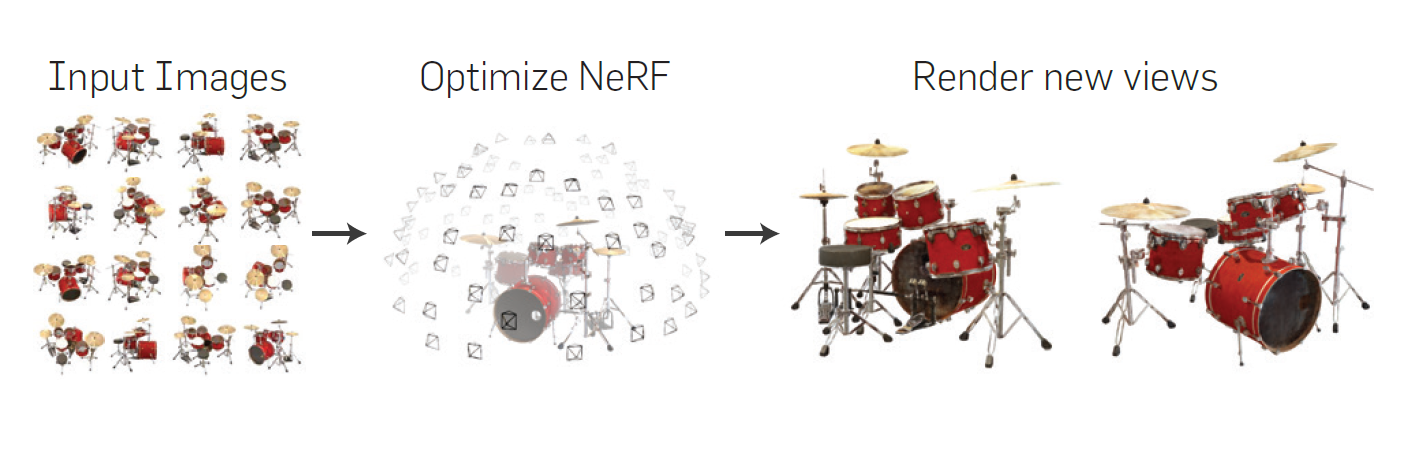
\includegraphics[width=0.9\textwidth]{Figures/Optimized NeRF.PNG}
  \caption[Illustration of Optimized NeRF]{This image illustrates a technique for refining a continuous 5D neural radiance field representation (comprising volume density and view-dependent color at each continuous point) of a scene, using a sequence of input photos. It employs volume rendering algorithms to collect samples of this scene representation along rays, enabling the scene to be portrayed from any viewpoint. Displayed below are 100 input views of the synthetic Drums scene, randomly selected from a surrounding sphere, followed by two novel views generated using the optimized NeRF representation \cite{mildenhall2021nerf}.}
  \label{fig:Optimized NeRF}
\end{figure}

\subsection{3D Gaussian Splatting and Compare With NeRF}
Neural radiance fields (NeRF) revolutionized computer graphics and 3D scene reconstruction by allowing for novel-view synthesis \cite{mildenhall2021nerf, avidan1997novel}. NeRF, based on deep learning and computer vision, can generate lifelike scenarios from sparse input views, creating a new paradigm in image synthesis.
However, NeRF, like any new technology, has faced hurdles and limits, particularly in terms of computing efficiency and control. 3D Gaussian splatting (3D GS) is a paradigm-shifting approach that redefines scene representation and rendering, rather than just incremental improvements \cite{kerbl20233d}. Prior to NeRF, novel-view synthesis focused on light fields and basic scene reconstruction algorithms \cite{gortler2023lumigraph, buehler2001unstructured}. Initial approaches were hampered by their reliance on deep sampling and structured capture, which made it difficult to handle complicated scenes and lighting. Structure-from-motion (SfM) and multi-view stereo (MVS) techniques improved 3D scene reconstruction and paved the way for advanced view synthesis
 \cite{snavely2006photo, goesele2007multi}. NeRF marks a significant advancement in this field. NeRF uses neural networks to map spatial data to colors and density. NeRF's success relied on its capacity to provide continuous, volumetric scene function, resulting in remarkable detail and realism. However, the implementation came at a cost. NeRF approaches were computationally costly, necessitating lengthy training and significant rendering resources, particularly for high-resolution results \cite{chen2022tensorf,garbin2021fastnerf,reiser2021kilonerf,takikawa2021neural, barron2022mip, muller2022instant}. 3D GS arose in response to these issues. Although NeRF excelled at creating photo realistic images, there was a growing demand for quicker and more efficient rendering methods, particularly for real-time applications. 3D GS introduced a revolutionary scene representation technique that employs millions of 3D Gaussian. Compared to implicit coordinate-based models, 3D GS uses explicit representations and parallelized workflows for efficient calculation and rendering \cite{mildenhall2021nerf,henzler2019escaping, sitzmann2019deepvoxels}.3D GS innovates by combining differentiable pipelines with point-based rendering approaches \cite{pfister2000surfels,wiles2020synsin}. Using learnable 3D Gaussians in scene representation preserves the desirable properties of continuous volumetric radiance fields for high-quality image synthesis while avoiding the computational overhead of rendering in empty space, which is a common drawback in traditional NeRF methods \cite{chen2024survey}. The emergence of 3D GS marks a significant shift in scene representation and rendering in computer graphics, beyond only technical advancements.
3D GS allows for real-time rendering without sacrificing visual quality, making it suitable for various applications such as virtual reality, augmented reality, and real-time cinematic rendering \cite{kalkofen2008comprehensible,patney2016towards,albert2017latency}. This technique has the potential to improve existing applications and enable new ones that were previously not possible due to computational constraints. Furthermore, 3D GS's explicit scene representation provides unparalleled control over complicated scenes with intricate geometry and changing lighting conditions \cite{chabra2020deep,wang2021learning}. 3D GS's control and edit-ability, along with its efficient rendering process, make it a transformational force in defining future improvements in the industry \cite{chen2024survey}.



\subsection{Image Segmentation}
Image segmentation is a popular research subject in computer vision, serving as the foundation for pattern recognition and picture understanding. Image segmentation has applications in various fields, including driver-less vehicles \cite{kabiraj2023number}, medical technology \cite{zhao2021voxelembed, jin2020deep}, search engines \cite{yao2021compound}, industrial inspection, and augmented reality. 
Image segmentation is a crucial step in comprehending natural scenes and is a popular study topic in image processing. It involves splitting a picture into meaningful, non-overlapping areas.Image segmentation involves three stages: traditional segmentation, collaborative segmentation, and semantic segmentation using deep learning as you can see in Figure \ref{fig:Categories of Image segmentation}. Image segmentation identifies areas of interest (ROIs) based on various attributes in an image. Humans perceive these zones as meaningful and non-overlapping. Image segmentation presents two challenges: (1) defining "meaningful regions" due to uncertainty in visual perception and human comprehension, making it an ill-posed problem; and (2) effectively representing objects in an image. Pixels in digital photos can be combined to create bigger sets based on color, texture, and other characteristics. These are known as "pixel sets" or "superpixels". Low-level picture features indicate local attributes, but obtaining global information (e.g., shape and position) from them is challenging.
\cite{yu2023techniques}

 
\begin{figure}[H]
  \centering
  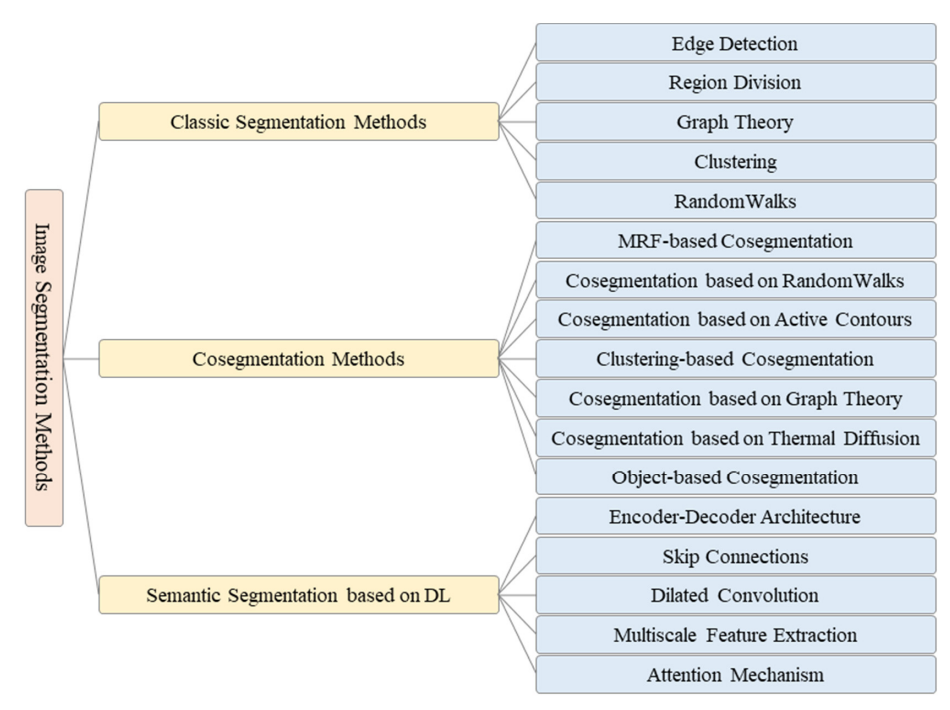
\includegraphics[width=0.9\textwidth]{Figures/categories of image segmentation method.PNG}
  \caption[Illustration of categories of image segmentation ]{This picture shows categories of image segmentation \cite{yu2023techniques}.}
  \label{fig:Categories of Image segmentation}
\end{figure}

\subsection{3D or Video Segmentation}
3D geometric data can be represented as point clouds, meshes, voxel grids, depth maps, parametric models, or RGB-D images. Segmenting 3D data can be hard, with several techniques available for different representations. Video sequences can be considered 3D data, as time is a third dimension. As still-image segmentation techniques improve, video segmentation is becoming increasingly popular.
Using still-image segmentation methods on video frames might be computationally expensive and fail to capture the temporal continuity of the content. Segmenting 3D/video data entails assigning labels to each minimal unit. Minimum unit can be a voxel, point, mesh or pixel within a video frame.In addition to practical picture segmentation applications, 3D segmentation is used in robotics and augmented/virtual reality \cite{wang2022comprehensive}. 





\subsubsection{Voxel-based Semantic Segmentation}
Deep learning has achieved significant success in picture, audio, and text recognition. However, few studies have investigated 3D large-scale point cloud classification. Unlike pictures, where the spatial relationships between pixels can be captured by sliding windows, the points in a point cloud are unstructured and the density is uneven. Parsing a 3D point cloud with noise, outliers, and under-sampling can be challenging. Liu \cite{liu20173dcnn} proposed a method called  3DCNN-DQN-RNN is intended to meet this difficulty. The model includes 3D convolutional neural network (3DCNN), Deep Q-Network (DQN), and residual recurrent neural network (RNN). The 3DCNN network learns visual, spatial, and contextual features from point cloud data at various scales, resulting in a 3D feature representation. The DQN uses trial-and-error to localize class objects through an eye window. The 3DCNN calculates a reward based on the eye window points, capturing significant features quickly. The eye window points' colors and coordinates are combined with the 3DCNN feature representation to create an input vector. This vector is then fed into the RNN to generate the final class labels. In the Figure \ref{fig:Liu Framework approach} the framework of this methods is shown. 
\begin{figure}[H]
  \centering
  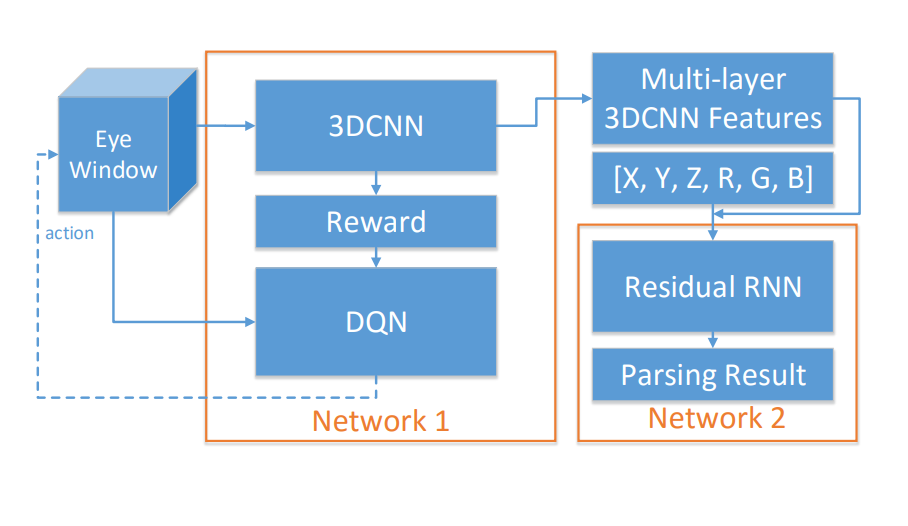
\includegraphics[width=0.9\textwidth]{Figures/Framework of Liu proposed approach.PNG}
  \caption[Illustration of Liu framework ]{This picture shows Liu framework approach that (X, Y, Z) and (R, G, B) representing 3D coordinate and RGB colors of each point in the original point cloud. \cite{liu20173dcnn}.}
  \label{fig:Liu Framework approach}
\end{figure}

\subsubsection{Point Cloud-based Semantic Segmentation}
3D point cloud segmentation divides point clouds into homogeneous zones, where points have similar attributes. Segmenting point cloud data is problematic due to significant redundancy, inconsistent sample density, and lack of explicit structure. This topic has multiple applications in robotics, including intelligent vehicles, autonomous mapping, and navigation \cite{nguyen20133d}. To handle point clouds, CNNs cannot be used directly and must be converted to other forms or adjusted to allow for data permutations.  Distances between points can help segmentation models identify objects or clusters in 3D space due to their variability \cite{wang2022comprehensive}. 

\begin{figure}[H]
  \centering
  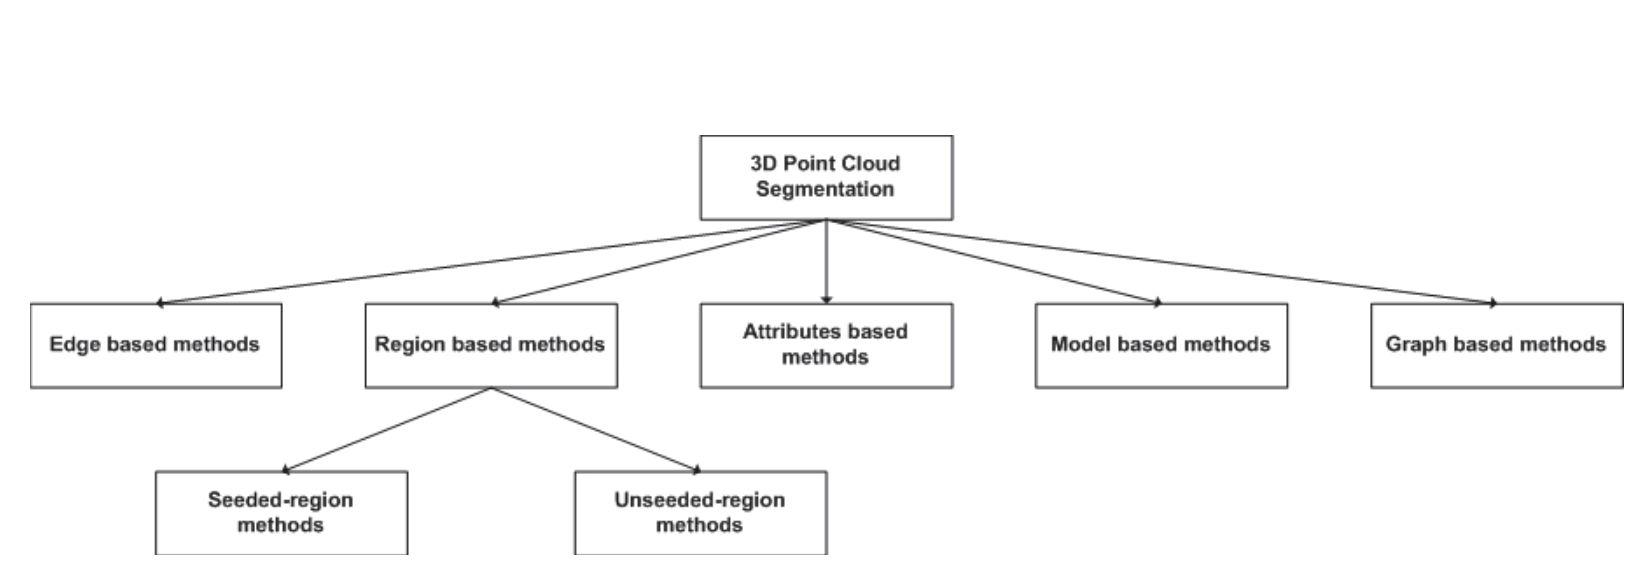
\includegraphics[width= 1.0\textwidth]{Figures/Taxonomy of 3D point cloud Segmentation methods.PNG}
  \caption[Illustration of Taxonomy of 3D point cloud Segmentation methods ]{This picture shows Taxonomy of 3D point cloud Segmentation methods \cite{nguyen20133d}.}
  \label{fig:Taxonomy of 3D point cloud Segmentation methods}
\end{figure}
 
\subsubsection{Semantic Segmentation by Robots}

Robots require a thorough understanding of their surroundings before interacting with the world. The accuracy with which a robot performs a task, navigates, or communicates is highly dependent on how well it understands its surroundings. Understanding context is vital for operating safely in varied situations \cite{premebida2018intelligent}. Accurately interpreting the surroundings is tough, particularly in complex and dynamic metropolitan environments. In these situations, robots are expected to complete their tasks perfectly despite encountering a variety of agents and objects. The process becomes more challenging when the appearance of the scene changes with lighting and weather conditions \cite{valada2020self}. Scene understanding in robotics entails identifying, localizing, and describing the elements that make up the environment, as well as their characteristics and dynamics. Because of the potential benefits for a wide range of applications, research on novel automatic scene interpretation systems has increased significantly during the last ten years. Advances in deep learning, open-source datasets, and increased computational resources have led to rapid improvements in scene interpretation approaches \cite{premebida2018intelligent}. 
visual classification is a prime example of technological advancements in determining visual content. This classification task's output can be considered a high-level representation of the scene, allowing for the identification of the numerous items present by assigning them a class label. Object detection is a mid-level feature that uses bounding boxes to classify and localize items in a picture, providing additional details. Although this assignment provides a more detailed representation of the scene, it is still unable to offer critical information or item properties such as object shape. Object segmentation is a related task that provides the shape of an object within a bounding box based on its segmented boundaries. Figure \ref{fig:From input image to semantic segmentation} shows an overview of various perceptive tasks\cite{hurtado2022semantic}.

\begin{figure}[H]
  \centering
  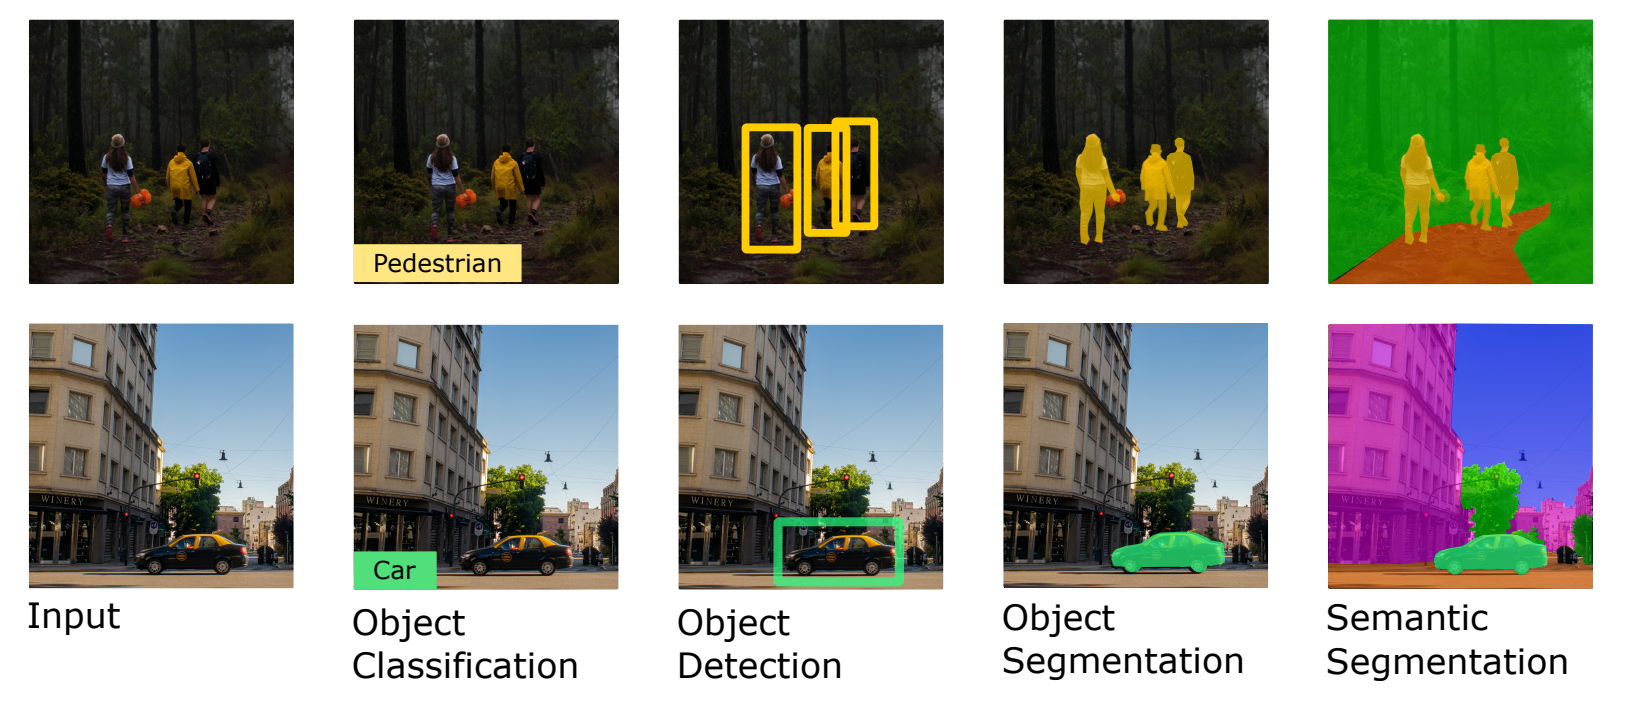
\includegraphics[width= 1.0\textwidth]{Figures/From input image to semantic segmentation.PNG}
  \caption[Illustration of From Input Image to Semantic Segmentation ]{In this picture each row displays an example of an input image and its matching output for various scene interpretation tasks. Object classification determines "what" items are in the image, whereas object detection predicts "where" they are, and object segmentation produces a mask indicating the shape of the object. Semantic segmentation enhances the input image by predicting the labels for all pixels, including the background.
 \cite{hurtado2022semantic}}
  \label{fig:From input image to semantic segmentation}
\end{figure}













\cleardoublepage


\chapter{Methodology}


\noindent In this chapter, I will discuss the approach employed in the thesis. Before delving into each sub-process, we'll go over the project's basic flow. 


\section{Project Overview for 360$^{\circ}$ Camera Pipeline}


\begin{figure}[H]
  \centering
  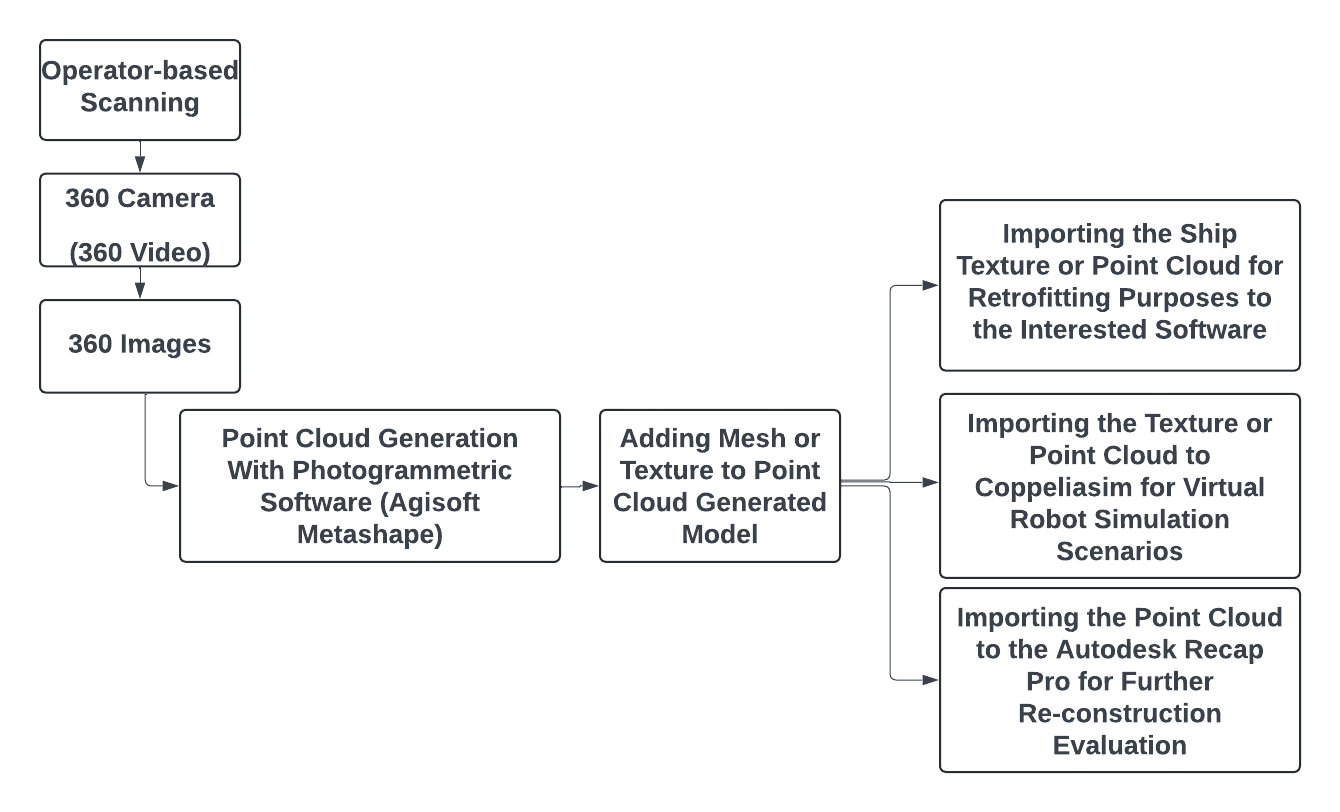
\includegraphics[width= 1.0\textwidth]{Figures/Project Flowchart.png}
  \caption[Illustration of Project Overview ]{Project Flowchart}
  \label{fig:Project Flowchart}
\end{figure}

In Figure \ref{fig:Project Flowchart}, I covered the project's overall outline, and the flow chart's square-shaped processes reflect sub-processes, which will be examined further in this chapter.


\subsection{Scanning with 360$^{\circ}$ Camera}
The first step that I need in this project is the scanning an asset or a scene to make a virtual point cloud of that object. Then I have my point could to make a 3D model. My industrial partner used QooCam 8K as you can see in Figure \ref{fig:QoooCam8K picture} for scanning the scene.  
\begin{figure}[H]
  \centering
  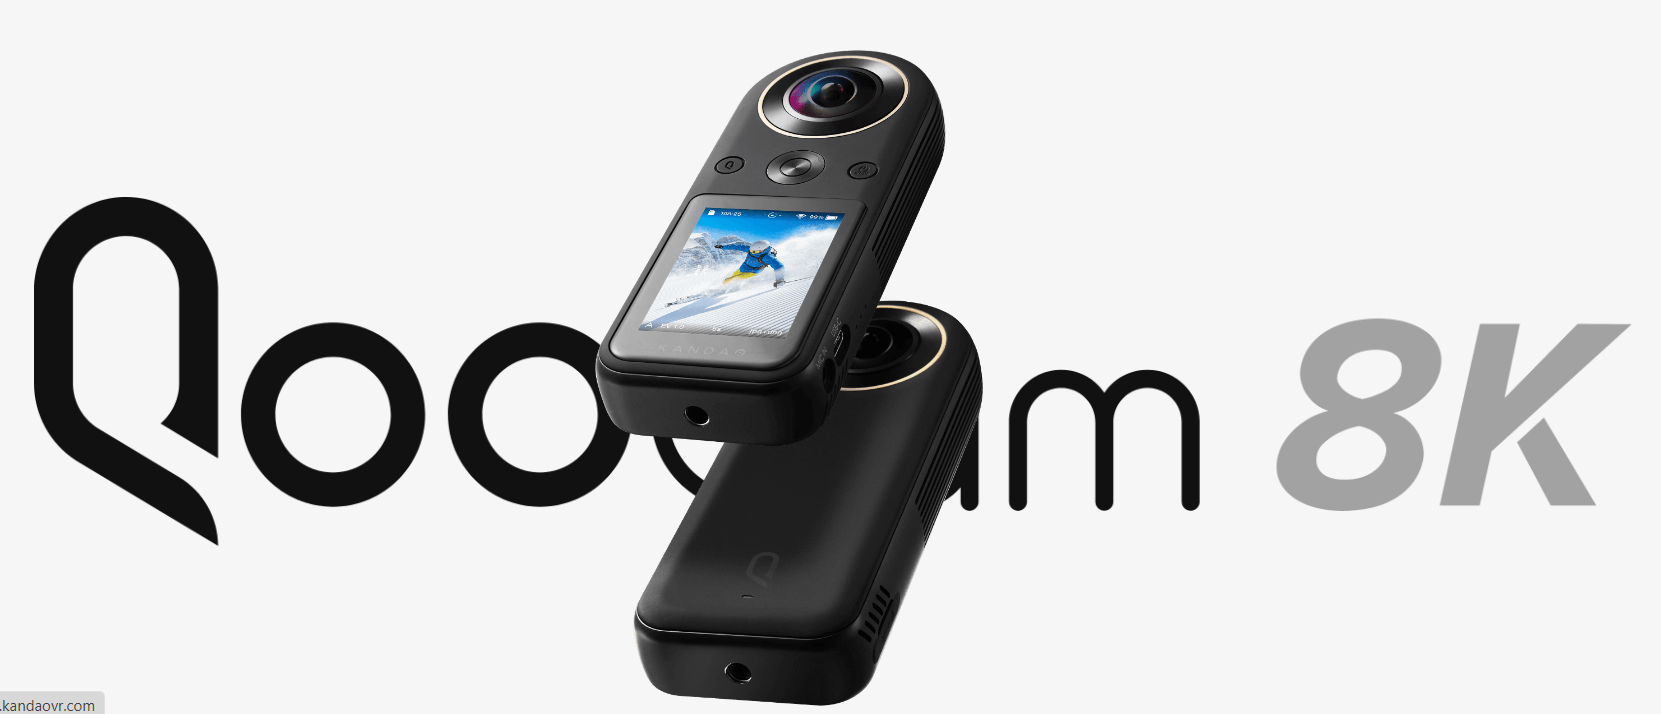
\includegraphics[width= 1.0\textwidth]{Figures/QooCam8K.PNG}
  \caption[Picture of QooCam8K]{Picture of QooCam8K \cite{QooCam8K}}
  \label{fig:QoooCam8K picture}
\end{figure}
\noindent In the below Figure \ref{fig:QooCam8K Specification}, the specification of this 360 camera is shown:

\begin{figure}[H]
  \centering
  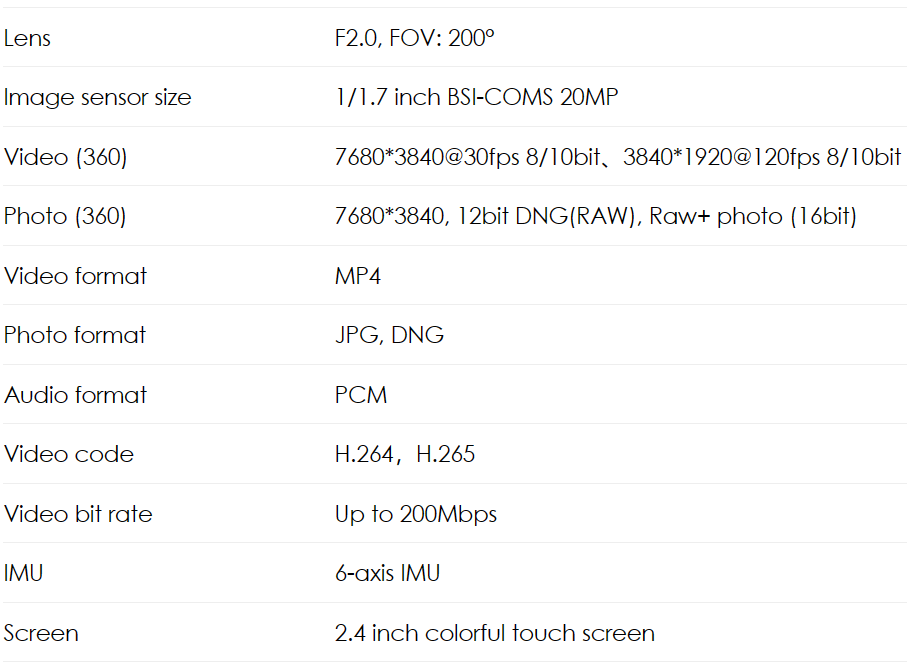
\includegraphics[width= 1.0\textwidth]{Figures/QooCam8KSPEC.PNG}
  \caption[Picture of QooCam8K Specification]{Picture of QooCam8K Specification \cite{QooCam8KSPEC}}
  \label{fig:QooCam8K Specification}
\end{figure}
 \textbf{Camera Features:} \\
I try to explain some features of this camera that is good to know for further work:
\begin{itemize}
    \item  \textbf{Lens F2.0}: F2.0 refers to the camera's aperture size. F2.0 permits more light to reach the image sensor. This can be useful in low-light settings without a flash. In general, the lower the F number, the more expensive the lens, and an F2.0 lens transports twice as much light as an f/4 lens. In Figure \ref{fig:Aperture Scale} aperture scale has been shown.  
\begin{figure}[H]
  \centering
  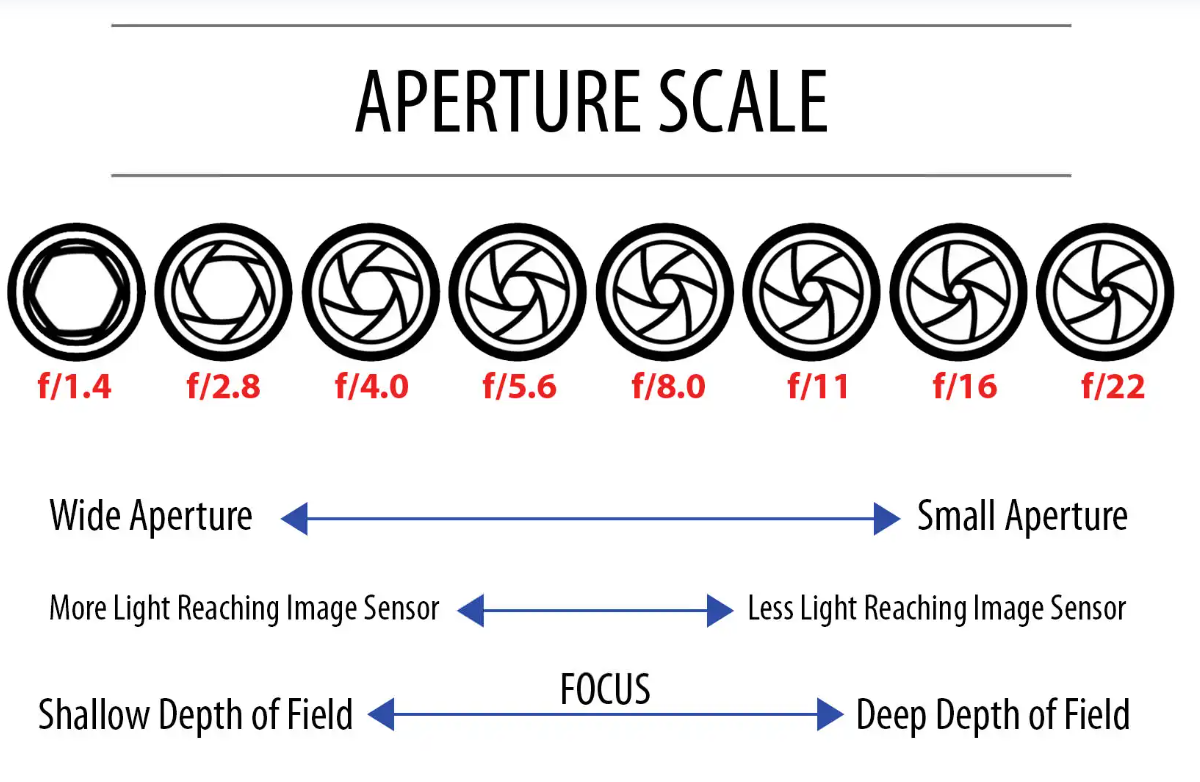
\includegraphics[width= 1.0\textwidth]{Figures/Aperture Scale.PNG}
  \caption[Picture of Aperture Scale]{Picture of Aperture Scale \cite{ApertureScale}}
  \label{fig:Aperture Scale}
\end{figure}
    
    The f-stop value indicates the amount of light entering the lens. Now comes the difficult part. Lower f-stop values allow more light to reach the lens. The greater the number, the less light. As a result, an aperture of f1.8 will let in far more light than an aperture of f2.2, resulting in superior, brighter photography in low-light situations such as night shots and some indoor photos. However, aperture affects more than just brightness. The depth of field is also directly related to the f-stop. A wider aperture, such as f1.8, produces a shallower depth of field, whilst a narrower aperture, such as f2.2, produces a deeper depth of field - so to extract the most detail from a shot, use the narrowest aperture \cite{lens}.


    \item  \textbf{FOV}: The field of view (FOV) is the open, viewable region that a person may see with their eyes or through an optical instrument like a camera. The maximum area that an optical instrument can capture is known as its field of view (FOV). FVO is related to two factors, the focal length of the lens and the sensor size. The focal length of a lens is the distance between the lens and the image being focused on the sensor. A bigger sensor provides a broader field of view at the same working distance. Changing the sensor size might alter the FOV. The sensor size is determined by the number and size of its pixels. Larger sensors produce a better image and have a higher resolution, whereas smaller sensors have a lower depth of field (DOF), resolution, and pixel size \cite{FOV,Fov}. In the Figure \ref{fig:Field of View of a Camera Lens} it shown the relation between field of view, focal length and sensor. 

 \begin{figure}[H]
  \centering
  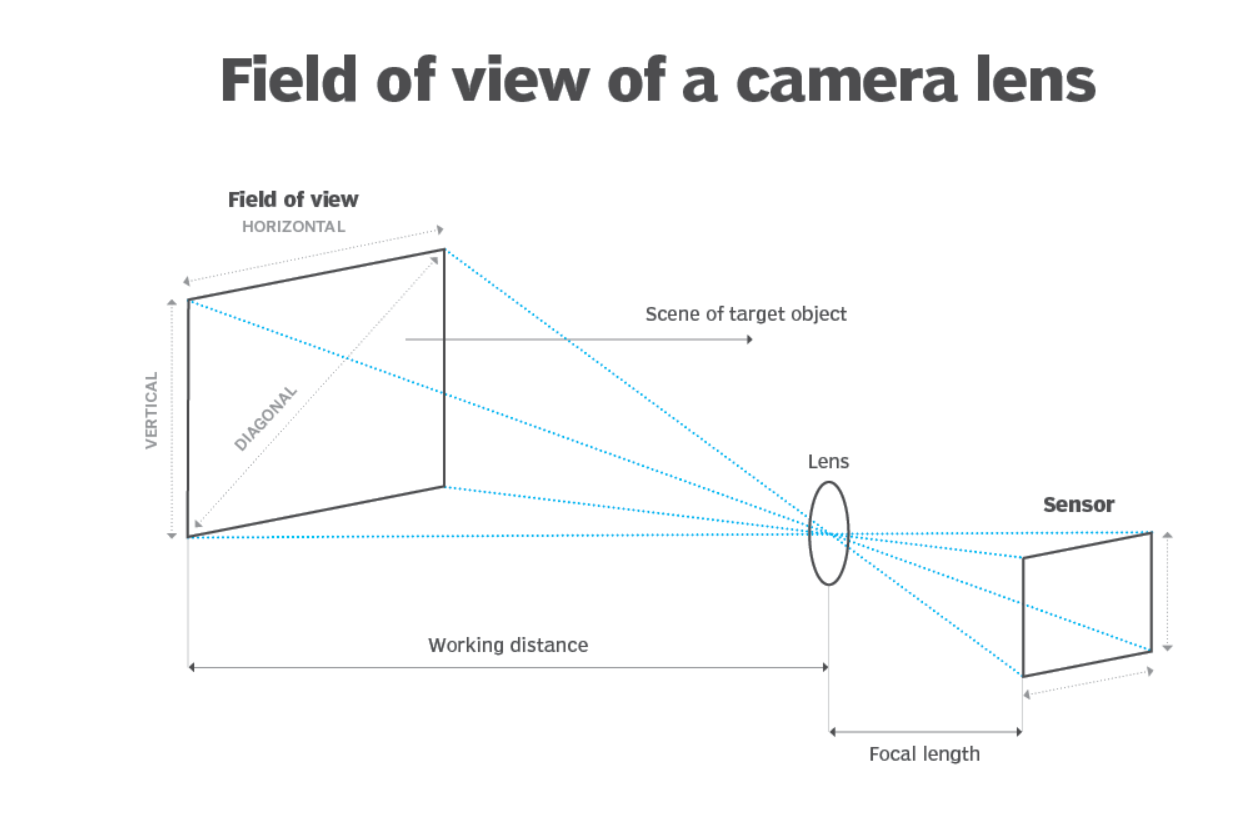
\includegraphics[width= 1.1\textwidth]{Figures/Field of View.PNG}
  \caption[Picture of Field of View of a Camera Lens]{Picture of Field of View of a Camera Lens \cite{FOV}}
  \label{fig:Field of View of a Camera Lens}
\end{figure}

    \item  \textbf{8K 30FPS or 4K 120FPS}:
QooCam8K is widely considered for 8K video recording with 30 frame per second or 4k with 120 frame per second.
In Figure \ref{fig:Different Resolution} the difference between the resolutions are visualized.
\begin{figure}[H]
  \centering
  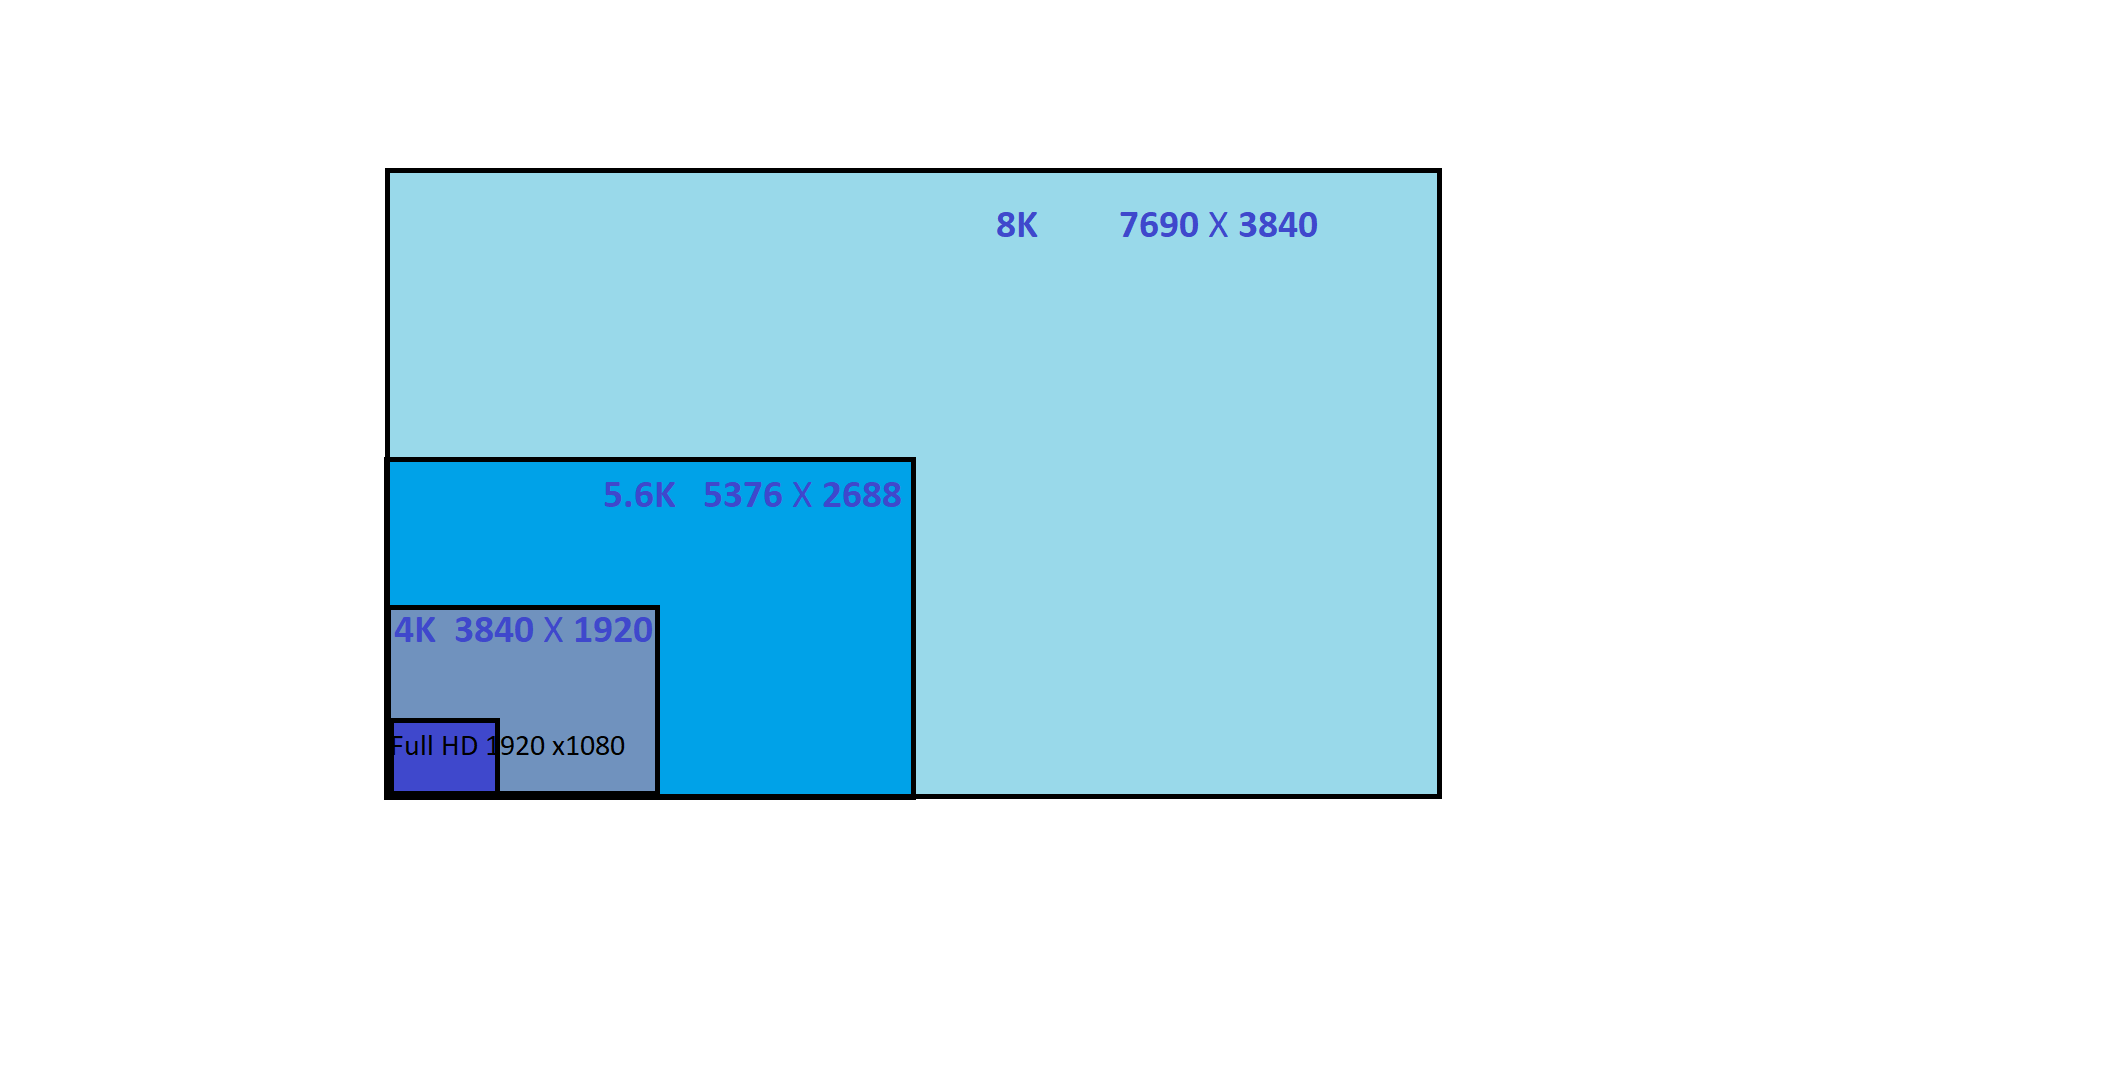
\includegraphics[width= 1.2\textwidth]{Figures/8K.PNG}
  \caption[Picture of Different resolutions]{Picture of Different Resolution}
  \label{fig:Different Resolution}
\end{figure}
 \noindent 4K 120FPS delivers the most cinematic 360 slow motion. Activities include skateboarding, paragliding, motocross, climbing, cycling, skiing, and surfing.Capture life's moments easily and turn them into spectacular slow motion.
    \item \textbf{10-Bit or 8-Bit Quality}:
    Color depth, also known as bit depth, is one of the parameters that define the quality of an image, whether still or video. They are the same thing. This is essentially a measure of how many shades and colors the camera can record; all other factors being equal, the more colors there are, the more complex and high-quality the footage can be. All photos captured by a digital camera contain red, green, and blue color information, and it is the combination of these color 'channels' that produces a full color image. So, when the camera is set to record in 8-bit video mode, it may capture footage with 256 levels for each color. This translates to a possibility of more than 16.7 million colors. If you set the quality to 10-bit video, you'll be capturing 1024 levels of color in each channel, with the potential for just over a billion different colors. However, it is worth noting that there is nothing wrong with 8-bit color. In fact, it is the style utilized in practically all of the videos you see on television or online.
 \cite{10Bit}. In Figure \ref{fig:Picture of Difference Betwwen 10-Bit and 8-Bit Video} the difference between 10-Bit and 8-Bit is more clear. 
\begin{figure}[H]
  \centering
  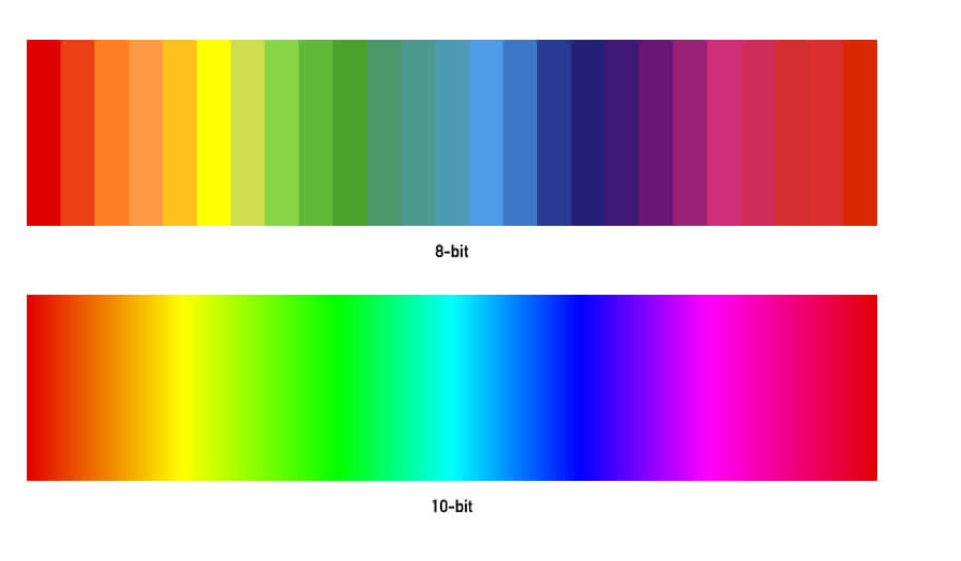
\includegraphics[width= 1.2\textwidth]{Figures/Bit.PNG}
  \caption[Picture of Difference Between 10-Bit and 8-Bit Video]{Picture of Difference Between 10-Bit and 8-Bit Video \cite{10Bit}}
  \label{fig:Picture of Difference Betwwen 10-Bit and 8-Bit Video}
\end{figure}
 
\end{itemize}
With QooCam8K scanned a hallway, in Figure \ref{fig:360 degree camera} the picture of hallway from 360 degree camera is shown.

\begin{figure}[H]
  \centering
  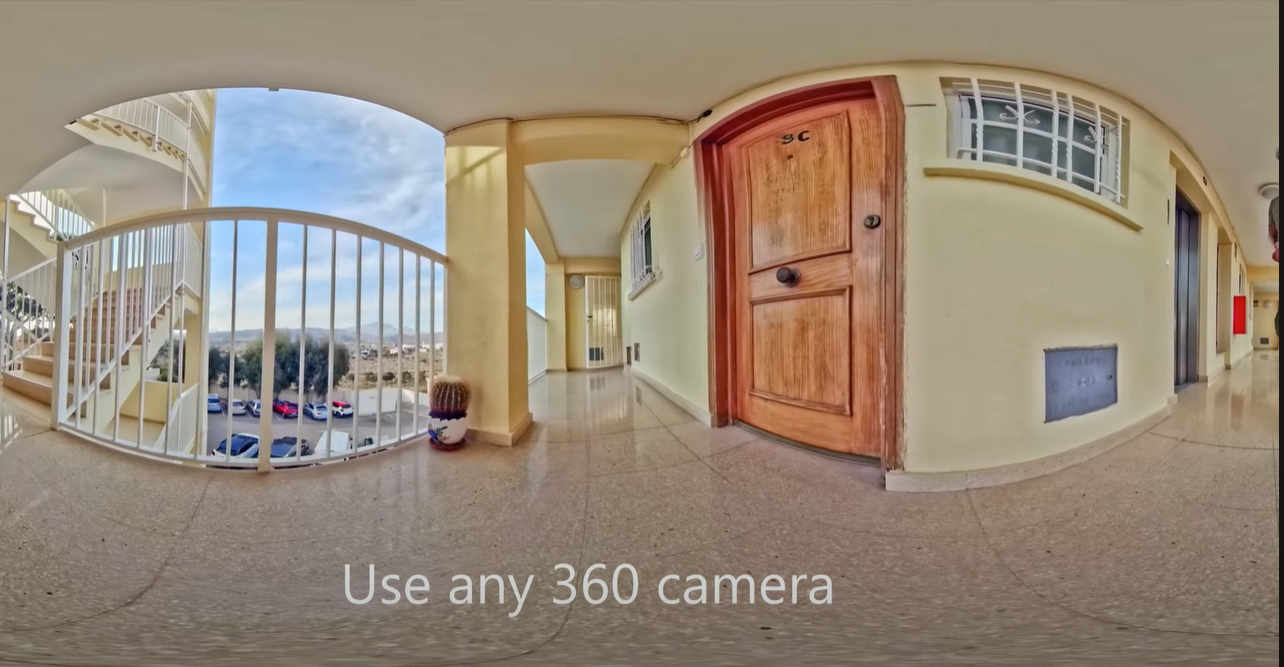
\includegraphics[width= 1.0\textwidth]{Figures/hallscan4.PNG}
  \caption[Picture of Hallway from 360 deegre camera]{Picture of hallway from 360 degree camera}
  \label{fig:360 degree camera}
\end{figure}
\noindent The hallway scan is made by ADAPA360 company as my industrial partner company. https://www.youtube.com/watch?v=5iUppdgs6TI \cite{ADAPA360}.\\

\noindent After scanning of the hallway with human-operator with low-speed  with 360 degree camera, then the scanned film imported to the Agisoft metashpe software for processing. This software make many frames of that footage, first aligned them and then stitch each image with neighbors images. Finally the point cloud is ready. It is also possible to visualize the point cloud in other software like Cloud Compare and Meshlab. In Figure \ref{fig:Camera Alignment in Agisoft} the camera alignment concept is visualized.  \\
\begin{figure}[H]
  \centering
  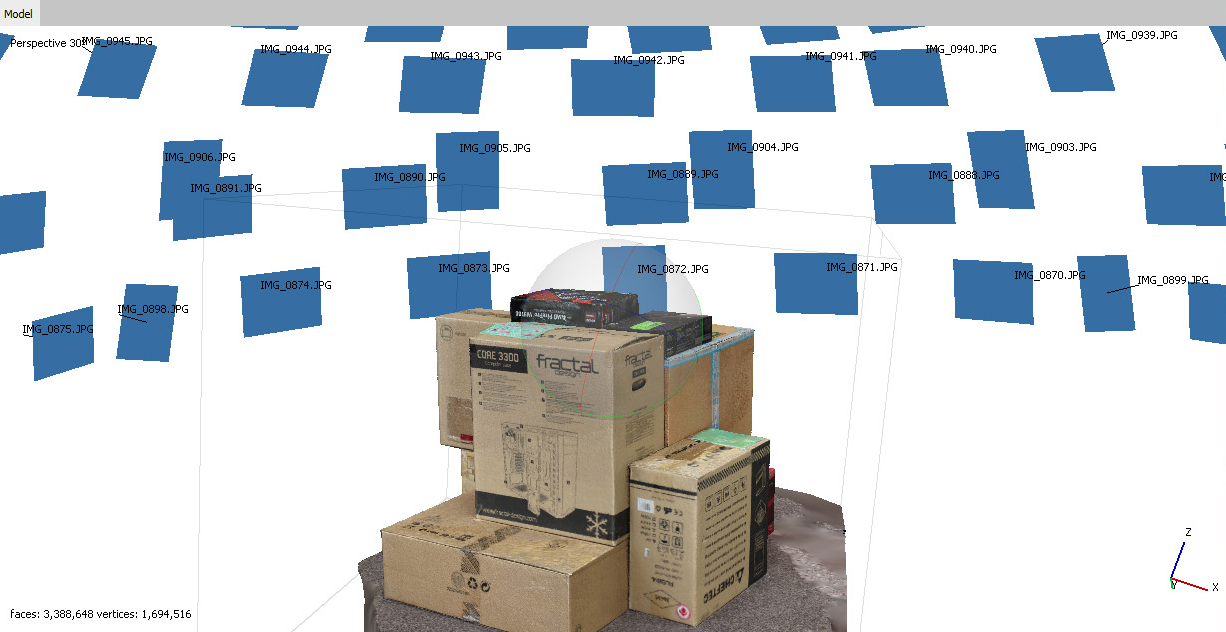
\includegraphics[width= 1.0\textwidth]{Figures/AgisoftCameraAlign.PNG}
  \caption[Camera Alignment in Agisoft]{Camera Alignment in Agisoft}
  \label{fig:Camera Alignment in Agisoft} \cite{Agisoft}
\end{figure}






 

%goal finding during avoiding the obstacles with different arrangement in the way. I used two algorithms 
\subsubsection{Concept for an UGV with Laser Scanner for Rescue Operations }
Imagine an autonomous ground robot just with laser scanner and without vision sensor wants to help for rescue operation in an unknown environment, what does it need to start the search. So, An autonomous robot developed for rescue operations must have several critical capabilities. \\

In the first step, it should be able to move around, overcome barriers, and adapt to diverse terrains. This allows the robot to reach regions that would otherwise be inaccessible or unsafe to humans. \\ 

Second, the robot should be equipped with a laser scanning sensor to detect its surroundings. This enables the robot to recognize and avoid obstacles while also locating targets, which is critical for effective rescue missions. \\

Third, the robot must have a communication mechanism to provide information back to the control center. This gives real-time updates on its location, status, and findings, allowing the control center to make educated decisions.\\

Fourth, the robot should have a dependable power source that allows it to function for long periods of time. This ensures that the robot can continue to operate without interruption.\\

Fifth, the robot should be resilient and robust enough to endure the extreme conditions common in disaster zones. This ensures the robot's durability and efficiency in these demanding conditions.\\

Sixth, the robot should have some degree of autonomy, allowing it to make decisions and complete tasks without continual human assistance. This boosts operational efficiency while reducing the workload on human operators.\\

If I want to summarize the robot operation into three main steps, there will be perception of surrounding environment by sensors and after that is decision making process based on the give algorithms and then actuation or movement until fulfilling the goal. 

\subsection{Algorithms for Making Decision }
I have used two types of implemented techniques for obstacle avoidance and motion planning purposes in CoppeliaSim. One technique is called potential field with gradient descent and another traditional technique is more robust for target finding low possibility of robot trapping and called vector field histogram plus(VFH+). 

\subsubsection{Motion Planning with Potential Fields }

In this part I introduce concepts in potential fields, main features and issues with this method.  There are two main forces for calculation in potential field, one is attractive force and another one is repulsive forces. Based on these two forces and calculations of gradient of the potential field, possible to control the robot \cite{Potentialfield}.    
\begin{itemize}
    \item  \textbf{ Potential function: }
\end{itemize}
 This is a scalar function and depends on the robot configuration \textit{q}, goal $q_{g}$, and obstacles $q_{o}$:\cite{khatib1986real} \\

\begin{equation}
\begin{aligned}
U(q, q_g, q_0) = U_{\text{attr}}(q, q_g) + U_{\text{rep}}(q, q_0)  
\end{aligned}
\label{eqn:potential function}
\end{equation} \\

\begin{figure}[h]
    \centering
    \begin{minipage}{0.45\textwidth}
        \centering
        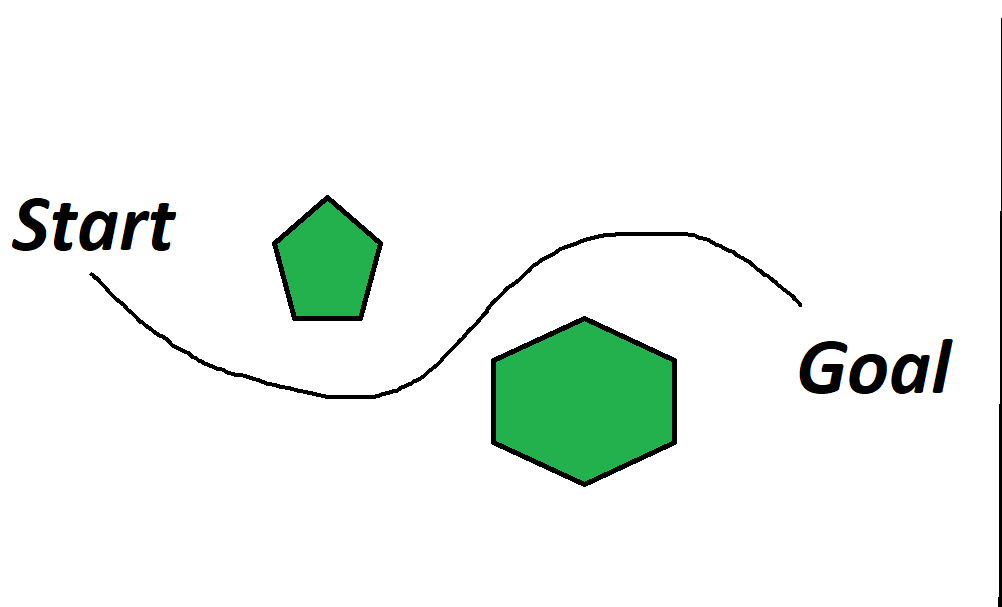
\includegraphics[width=0.9\textwidth]{Figures/graph.png} % first figure itself
        \caption{Start to Goal}
    \end{minipage}\hfill
    \begin{minipage}{0.45\textwidth}
        \centering
        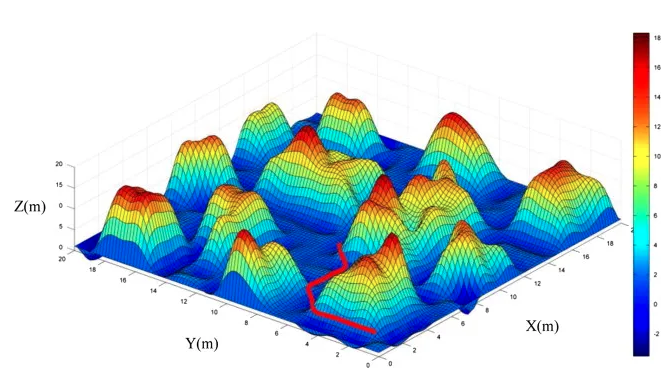
\includegraphics[width=0.9\textwidth]{Figures/graph2.PNG} % second figure itself
        \caption{Obstacles in 3D}
    \end{minipage}
\end{figure}

%------
\noindent \textbf {Attractive Potential Function}: This function depends on goal and robot configuration and based on this function the robots move towards the goal.
\\

\begin{itemize}
    \item  \textbf{ Quadratic Attractive Function (Parabolic): }\\
Quadratic function can take high values when the robot is far from the goal and the same is smooth in the vicinity og the goal.  
\begin{equation}
\begin{aligned}
U_{\text{attr}}(q, q_g) = \frac{1}{2} \epsilon_q d^2(q, q_g) \\
d(q, q_g) = \sqrt{(x - x_g)^2 + (y - y_g)^2}
\end{aligned}
\label{eqn:Quadratic Attractive Function}
\end{equation}  

     \item  \textbf{ Linear Attractive Function (Conic): }
The conic function is proportional to the distance between robot and the goal, however in the vicinity of the goal, the function will change abruptly.  
\begin{equation}
\begin{aligned}
U_{\text{attr}}(q, q_g) = \epsilon_c d(q, q_g)
\end{aligned}
\label{eqn: Linear Attractive Function}
\end{equation}  
\end{itemize}
\begin{figure}[h]
    \centering
    \begin{minipage}{0.45\textwidth}
        \centering
        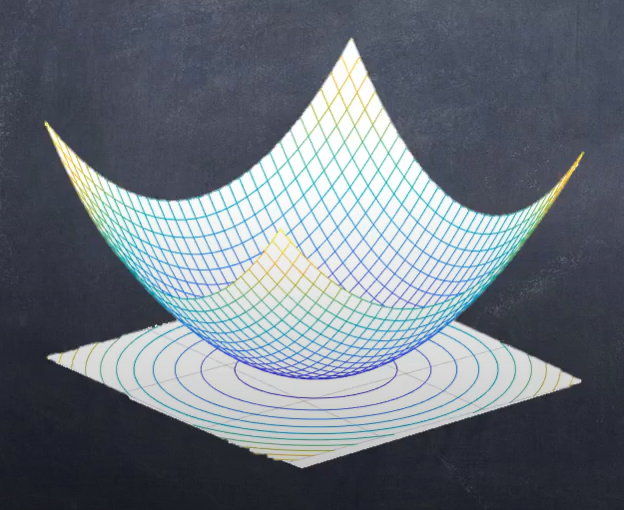
\includegraphics[width=0.9\textwidth]{Figures/Quad.PNG} % first figure itself
        \caption{Quadratic Function}
    \end{minipage}\hfill
    \begin{minipage}{0.45\textwidth}
        \centering
        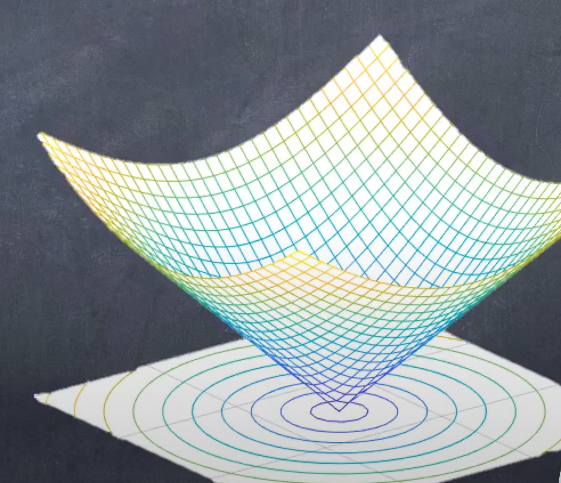
\includegraphics[width=0.9\textwidth]{Figures/Linear.PNG} % second figure itself
        \caption{Conic Function}
    \end{minipage}
\end{figure}

\begin{itemize}
      \item  \textbf{ Conic-parabolic Attractive Function: }
This function combines both conic and parabolic functions and define a distance threshold $Q_g$ and also a parabolic attractive constant. This function inside behaves parabolically which depends quadratically with the distance while from outside function behaves conically that it depends linearly with distance. 
\end{itemize}

\begin{equation}
\begin{aligned}
U_{\text{attr}}(q, q_g) = 
\begin{cases} 
\frac{1}{2} \epsilon_{q} d^2(q, q_g) & \text{if } d(q, q_g) < Q_g \\
Q_g \epsilon_{q} d(q,q_g) - \epsilon_{d} \frac{Q^2_g}{2} & \text{if } d(q, q_g) \geq Q_g 
\end{cases}
\end{aligned}
\label{eqn:Conic-parabolic attractive function}
\end{equation}  \\

\noindent \textbf {Repulsive Potential Function or Obstacle Avoidance Function}: This function parameters are dependent on the obstacle and robot configuration.This function avoids the robot from getting closer to the obstacles \cite{Pathplanning}.  

\begin{itemize}
      \item  \textbf{ Hyperbolic Repulsive Function: }
Repulsive function is defined by two distances, the first distance is beyond the specific distance that the robot has no influence on and the second distance is a minimum safety distance to avoid the obstacles, so if the robot has    
more distance than the threshold distance $Q_\text{inf}$ , the obstacles have no influence on it and if the robot is in area of the minimum distance $Q_\text{min}$ (safety distance) so the robot can not go closer to obstacle. And parameter $\epsilon_r$ modify how repulsive function effects to the robot. 
\end{itemize}

\begin{equation}
\begin{aligned}
U_{\text{rep}}(q, q_o) = 
\begin{cases} 
0 & \text{if } Q_{\text{inf}} \leq d(q, q_o), \\
\epsilon_r \left( \frac{1}{d(q, q_o)} - \frac{1}{Q_{\text{inf}}} \right) & \text{if } Q_{\text{min}} \leq d(q, q_o) \leq Q_{\text{inf}}, \\
\epsilon_r \left( \frac{1}{Q_{\text{min}}} - \frac{1}{Q_{\text{inf}}} \right) & \text{if } d(q, q_o) \leq Q_{\text{min}}.
\end{cases} 
\end{aligned}
\label{eqn: Hyperbolic Repulsive Function}
\end{equation}  \\

being $Q_{\text{min}}$ < $Q_{\text{inf}}$\\

\noindent \textbf {Total Potential Field}: This potential combines the attractive potential with the repulsive potential of obstacles, so the robot is attracted to a force field that pushes it towards the goal avoiding obstacles. 
\begin{equation}
\begin{aligned}
U(q, q_g, q_o) = U_{\text{attr}}(q, q_g) + \sum_i U_{\text{rep}}(q, q^{i}_o)
\end{aligned}
\label{eqn:Total Potential Field}
\end{equation} 
For the calculation of total potential function, I need distances to the goal and obstacle configuration and this can be done easily if a map is available but also considering sensor information. Total potential field can be used as state of control law with a known environment or as a sensor-based navigation method for global or local path-planning \cite{lu2014information}.  \\


\noindent \textbf {Gradient Descent}:
For planning a route,there is a need to follow the opposite direction of the gradient, because the gradient is a vector whose magnitude and direction will depend on the robot configuration, goal and obstacles. It is good to mention that locally the negative gradient will point in the direction that minimize the potential function (configuration with less energy),So the robot feels a force opposite to the gradient. \\
\begin{equation}
\begin{aligned}
\dot{q} = -\nabla U(q, q_g, q_o) = -\nabla U_{\text{attr}}(q, q_g) - \sum_i \nabla U_{\text{rep}}(q, q^{i}_o)
\end{aligned}
\label{eqn:Gradient Descent}
\end{equation} 

\noindent \textbf {Control Techniques}
\begin{itemize}
      \item  \textbf{ Force Control: }
To implement potential field technique, we need to compute the gradient of potential function, this gradient can be seen as a force that pushes the robot. In this case the effect of this force filtered by robot dynamic, so this type of control is generally smooth. And there would be some oscillations if the friction is not included in the dynamic of robot. 
\begin{equation}
\begin{aligned}
F = -\nabla U(q, q_g, q_o)
\end{aligned}
\label{eqn:Force Control}
\end{equation} 
      \item  \textbf{ Speed Control: }
Another typical alternative is to establish speed control so it means, here the speed is proportional to the gradient. The effect on the robot is independent of its dynamic which means robot is faster but it can produce sudden changes. In this case the most common implementation is the steepest descent method, it uses the unitary gradient vector and step size that the gradient step $lambda$ is a design parameter that can controls the amount of distance the robot can move \cite{LocalMinimum}.

\begin{equation}
\begin{aligned}
\dot{q} = -\nabla U(q, q_d, q_o) \\
q_{k+1} = q_k - \lambda \frac{\nabla U(q, q_d, q_o)}{\| \nabla U(q, q_d, q_o) \|}\\
\end{aligned}
\label{eqn:Speed Control}
\end{equation} 
\end{itemize}

\noindent \textbf {Local Minimum}\\
The attractive function has a single global minimum in the goal configuration; however, when combined with the repulsive function, local minimums may occur in some configurations that are difficult to predict if the entire configuration space is not well explored. This problem occurs where the gradient in the configuration becomes zero as a result of the balance of attracting and repulsive forces. Figure \ref{fig:Local Minimum} shows that there are some initial configurations from which the robot will not be able to reach the goal configuration. Local minimum are equilibrium points, so if we add some energy or little that might be enough to reach the goal configuration and the robot can escape from it. The type of this energy can be variant, there could be virtual forces, random movement, virtual objects or way-points.  

\begin{figure}[H]
  \centering
  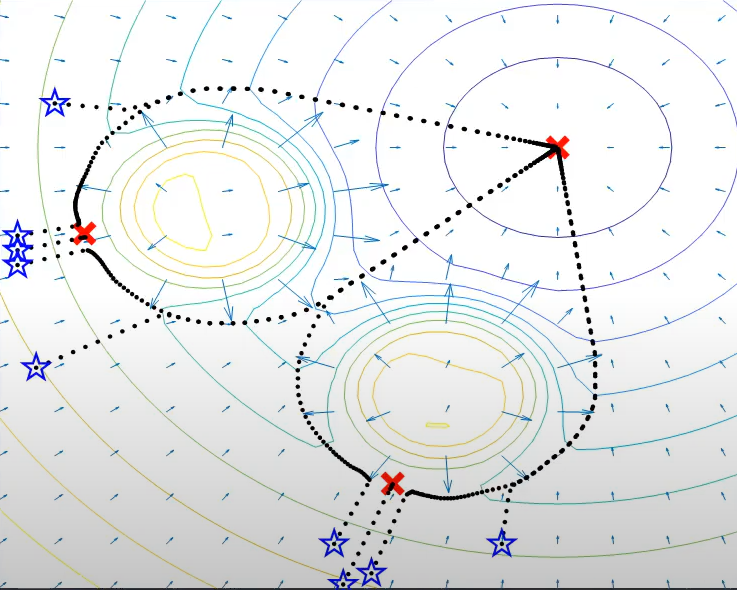
\includegraphics[width= 0.7\textwidth]{Figures/pot.PNG}
  \caption[Local Minimum]{Local Minimum} \cite{LocalMinimum}
   \label{fig:Local Minimum}
\end{figure}





\subsubsection{Motion Planning with Vector Fields Histogram plus (VFH+) an enhancement of VFH : }


  The vector field histogram (VFH) is a real-time obstacle avoidance system for mobile robotics. In VFH method there would be possible to make 2d occupancy map or cell histogram that enables for the incorporation of inaccurate measurements from sensors like ultrasound or laser and if 2d occupancy map or cell histogram is not available we can always use raw laser sensor data. In Figure \ref{fig:2d Occupancy Map} and Figure \ref{fig:cell histogram} sample of 2d occupancy map and cell histogram has been shown.
 

\begin{figure}[h]
    \centering
    \begin{minipage}{0.4\textwidth}
        \centering
        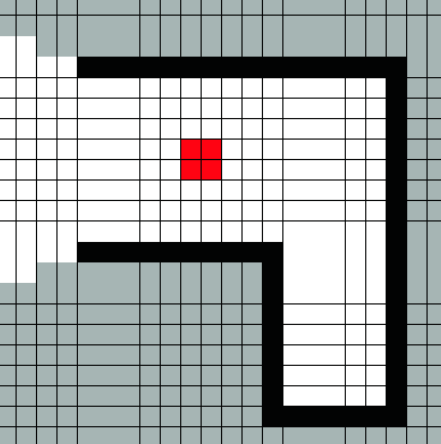
\includegraphics[width=0.9\textwidth]{Figures/2d Occupancy map.PNG} % first figure itself
        \caption{2d Occupancy Map \cite{Wang2018}}
        \label{fig:2d Occupancy Map}    
    \end{minipage}\hfill
    \begin{minipage}{0.5\textwidth}
        \centering
        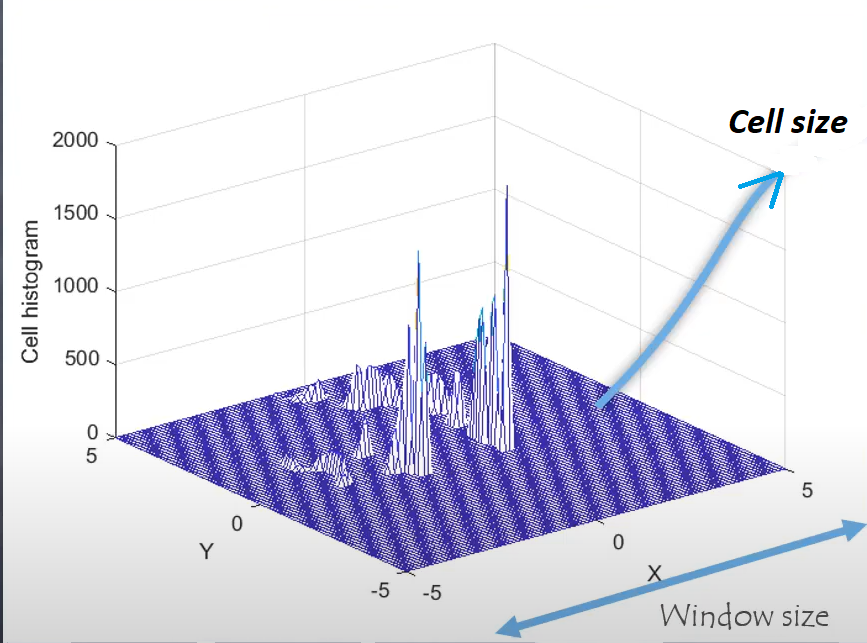
\includegraphics[width=0.9\textwidth]{Figures/cell histogram.PNG} 
        \caption{Cell Histogram \cite{Cellhistogram}} 
        \label{fig:cell histogram}
    \end{minipage}
\end{figure}

 \noindent The core concept of VFH method is to reduce this map to a polar histogram based on the preliminary ideas known as Virtual Field Force (VFF). Secondly valleys are detected in polar histogram to propose candidate directions to move and it means lower values of polar histogram in a given direction are less likely to face an obstacle. Also these valleys using threshold values and those sections that does not have threshold values means they are free sectors. When valleys have been detected are like set of sectors below the threshold and the one that is closest to the goal direction, will be selected and within that valley a direction according to the robot body size is selected to let the robot go forward. Now it should be distinguished that if it is wide or narrow valley\cite{VFH}. To understand how wide is a valley the VFH method improved to VFH+. VFH+ enhances the Vector Field Histogram (VFH) approach for real-time obstacle avoidance in mobile robots. The VFH+ approach improves robot trajectories and dependability. VFH+ simplifies parameter setting by accounting for robot width. VFH+ improves mobile robot trajectory accuracy, leading to increased reliability \cite{ulrich1998vfh+}. \\

   
 


\subsubsection{ Steps in VFH+ Method Implementation (Occupied Cells Detection and Obstacle Avoidance Method) }

Here I talked about all the VFH+ stages for data-reduction process that I need for computation of new direction toward goal with obstacle avoidance. \\

\textbf{ A. } First I need to make a cell histogram, whose values are updated based on the range sensor measurements.After several passes they will provide the certainty of the cells being occupied. Also I  can improve this stage by using occupancy maps which shows the likelihood of occupied cells. So the first stages of data reduction involves mapping the active region of the map grid to the principal polar histogram. The active region is a circular window (diameter Ws) that moves with the robot. The map grid treats each active cell's content as an obstacle vector. In the Figure \ref{fig:Histogram Grid Cells} shown an example of histogram grid cells and values. 
\begin{figure}[H]
  \centering
  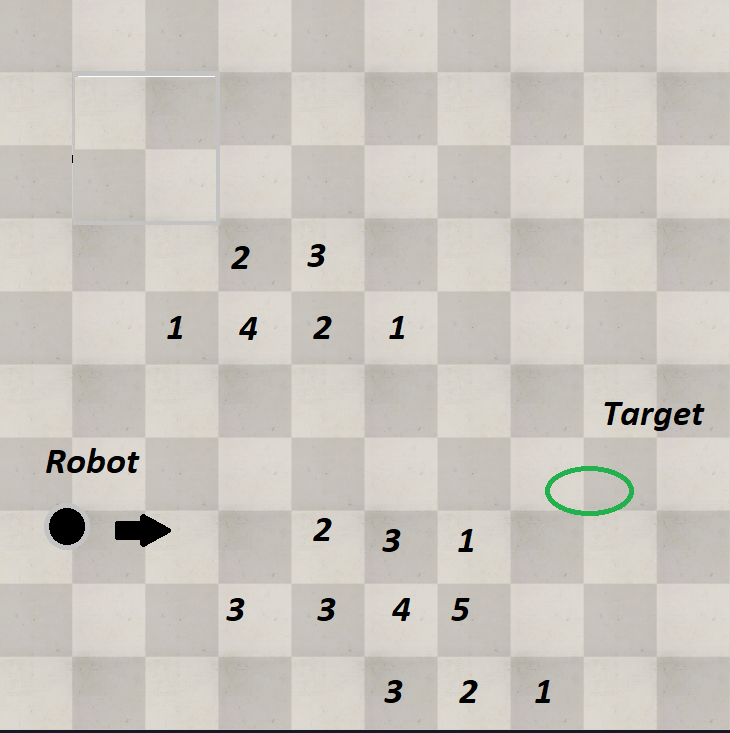
\includegraphics[width= 0.7\textwidth]{Figures/Grid.PNG}
  \caption[Histogram Grid Cells]{Histogram Grid Cells}
   \label{fig:Histogram Grid Cells} 
\end{figure}

\noindent \textbf{ B. } A 2d cell histogram will be converted to polar histogram that is a 1 dimensional histogram and in this process the size of the robot is taking into account.
For each cell a magnitude is computed depending on the cell distance to the robot and its occupancy likelihood and the magnitude are accumulated on their corresponding polar sector. In Figure \ref{fig:Active Cell's Magnitude and Assigned Sectors onto the Polar Histogram} a map of active cells on the polar histogram with each cell magnitude and the sectors have been shown. 
\begin{figure}[H]
  \centering
  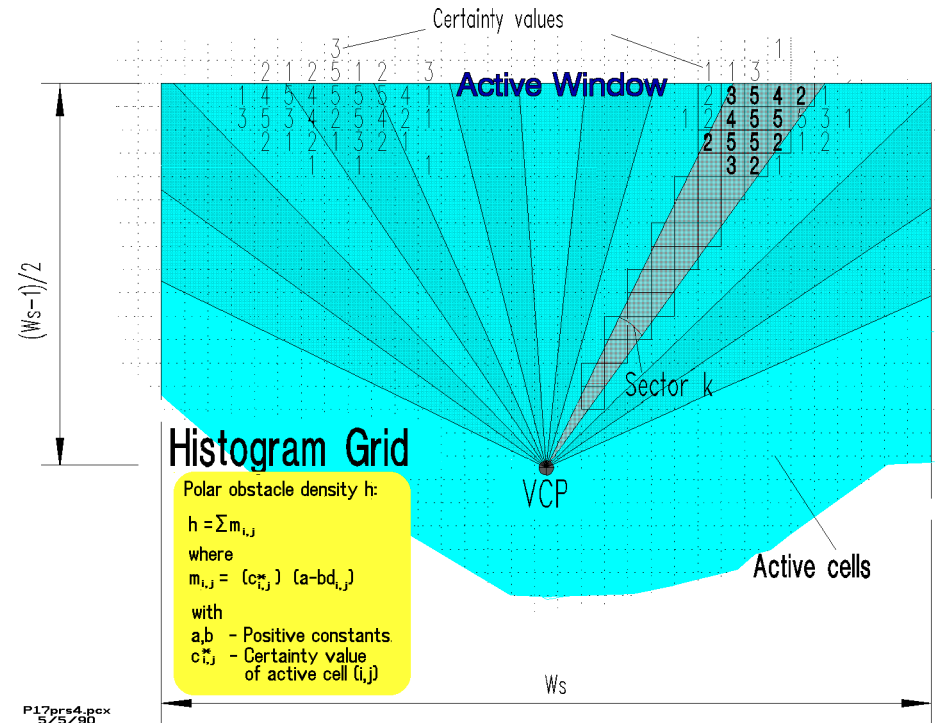
\includegraphics[width= 1.0\textwidth]{Figures/Active cells.PNG}
  \caption[Active Cell's Magnitude and Assigned Sectors onto the Polar Histogram]{Active Cell's Magnitude and Assigned Sectors onto the Polar Histogram}
   \label{fig:Active Cell's Magnitude and Assigned Sectors onto the Polar Histogram} \cite{Borenstein1991}
\end{figure}
\noindent Then it is possible to make 1d polar histogram with consideration of robot size as it is shown in Figure \ref{fig:Polar Histogram}. 
\begin{figure}[H]
  \centering
  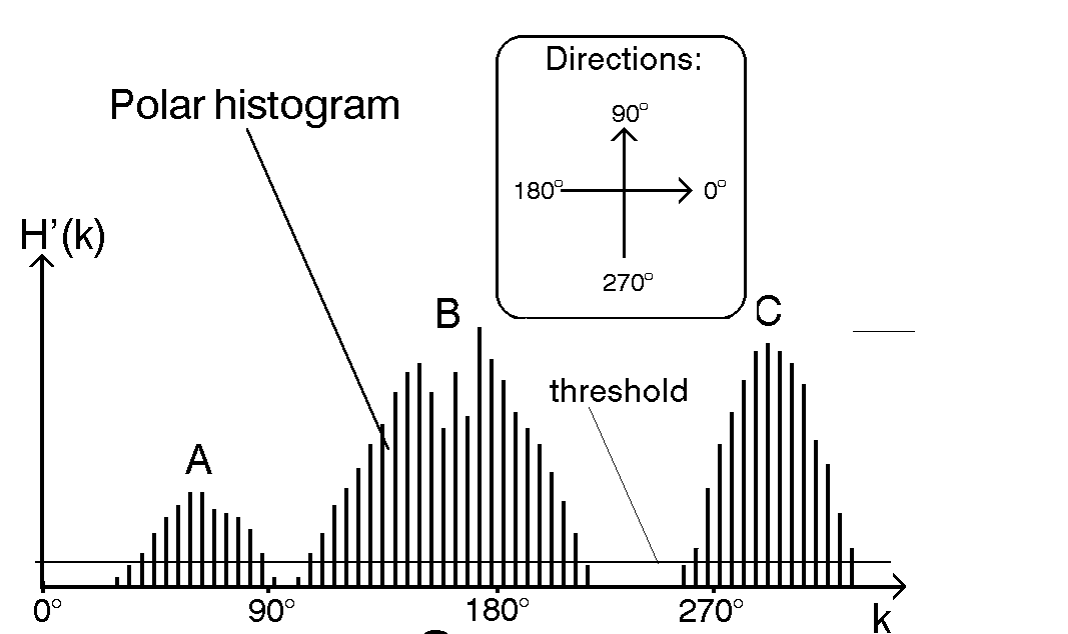
\includegraphics[width= 0.7\textwidth]{Figures/Polar Histogram.PNG}
  \caption[Polar Histogram]{Polar Histogram}
   \label{fig:Polar Histogram} \cite{Borenstein1991}
\end{figure}
\noindent \textbf{ C. } Next step is to making binary polar histogram to find the occupancy of sectors, for this purpose VFH+ method uses two thresholds to determine if a sector is occupied or free. If the value is more than the threshold the magnitude will be 1 and it means occupied and if the value is lower than the threshold the value is zero and means it is a free sector. If the values are between the thresholds ,the value of previous iteration will be used.  

\begin{equation}
\begin{aligned}
H_k^b = \begin{cases} 
1 & \text{if } H_k^p > \tau_{\text{high}} \\
0 & \text{if } H_k^p < \tau_{\text{low}} \\
H_k^p & \text{otherwise}
\end{cases}
\end{aligned}
\label{eqn:Speed Control}
\end{equation} 
In Figure \ref{fig:Binary Histogram} the binary histogram with thresholds is shown. 
\begin{figure}[H]
  \centering
  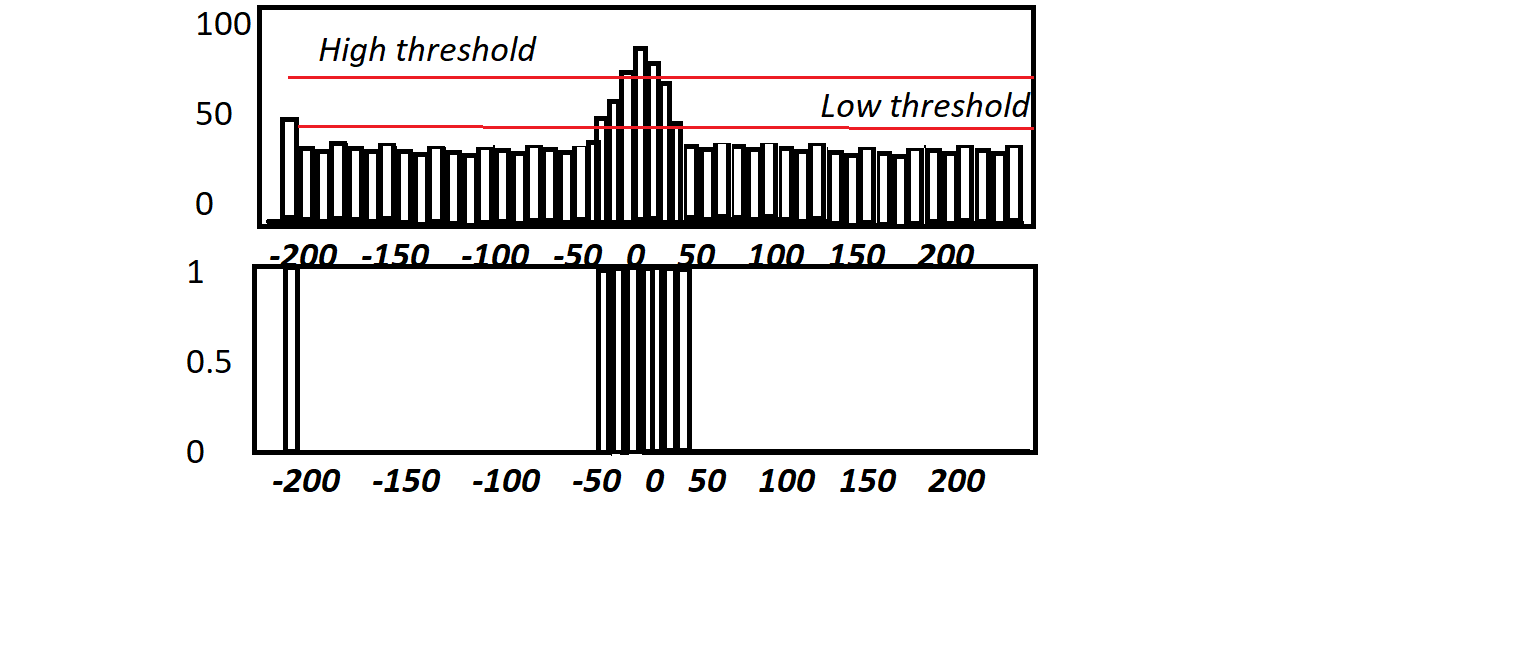
\includegraphics[width= 1.5\textwidth]{Figures/Binary histogram.png}
  \caption[Binary Histogram]{Binary Histogram}
   \label{fig:Binary Histogram} 
\end{figure}

\noindent \textbf{ D. }  The last histogram is the masked histogram, this histogram takes into account that the robot has some kinematic or dynamic constrains, therefore there is a minimum turning radius. This minimum turning radius imply that in-order to reach a free sector or sector that was categorized as a free in the binary histogram, I need to go through another sector that might be locked, then in that case those sectors will be also blocked. In Figure \ref{fig:2D Masked Histogram} and Figure \ref{fig:Binary and Masked Histogram}  visualized the the way that robot can decide between two obstacles by binary and masked histogram. As you can see the red zone in the masked histogram is marked as blocked direction because in order to reach those direction the robot must necessarily pass through the orange zone and due to minimum radius which is depicted in the blue circles in the  Figure \ref{fig:2D Masked Histogram}, this cannot be possible without colliding.   

\begin{figure}[H]
  \centering
  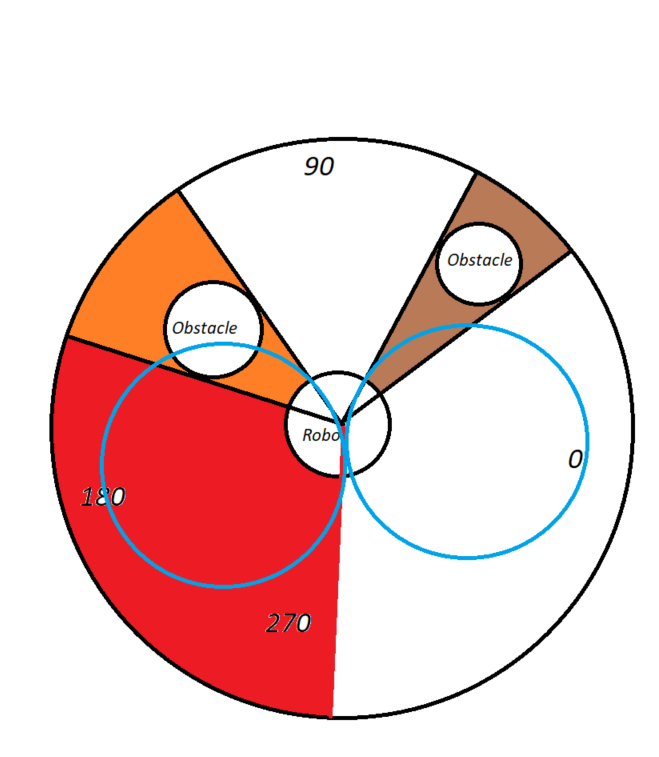
\includegraphics[width= 0.7\textwidth]{Figures/maskedcircle.PNG}
  \caption[2D Masked Histogram]{2D Masked Histogram}
   \label{fig:2D Masked Histogram} 
\end{figure}
\begin{figure}[H]
  \centering
  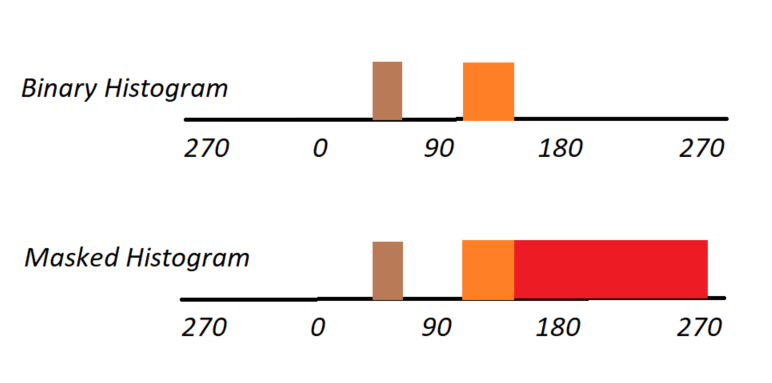
\includegraphics[width= 0.9\textwidth]{Figures/Binaryandmaskhis.PNG}
  \caption[Binary and Masked Histogram]{Binary and Masked Histogram}
   \label{fig:Binary and Masked Histogram} 
\end{figure}

\noindent \textbf{ E. } Once I have a masked histogram, then it is possible to detect the valleys which are set of sectors marked as free sectors. Two types of valleys are defined, narrow  and wide valleys. Narrow valley represent a region in which the robot can pass through but it is surrounded by obstacles, therefore this is only one possible direction which is just basically passed through the middle of the valley. A narrow valley shown in Figure \ref{fig:Narrow Valley in Histogram}. 

\begin{figure}[H]
  \centering
  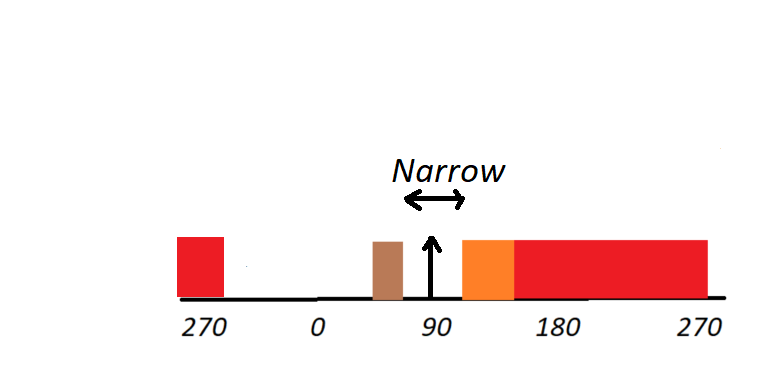
\includegraphics[width= 0.7\textwidth]{Figures/narrow.PNG}
  \caption[Narrow Valley in Histogram]{Narrow Valley in Histogram}
   \label{fig:Narrow Valley in Histogram} 
\end{figure}


\noindent On the other hand, there is wide valley which represents the region with obstacles far away from the robot, and in this case I usually can take three possible candidate directions to move through the left, the right edges or straight towards the goal if it is inside the valley. A wide valley shown in Figure \ref{fig:Wide Valley in Histogram}. 
\begin{figure}[H]
  \centering
  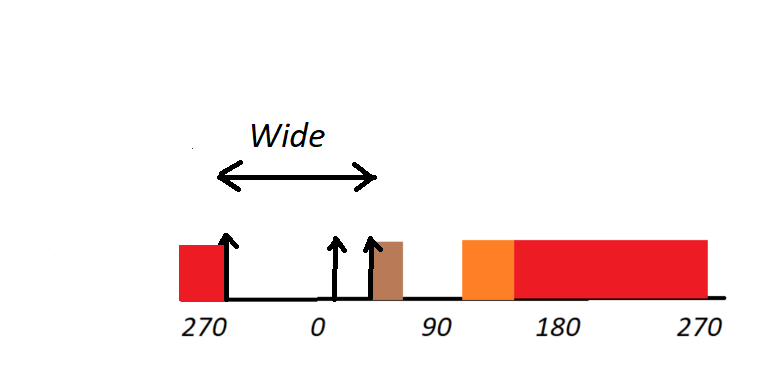
\includegraphics[width= 0.7\textwidth]{Figures/wide.PNG}
  \caption[Wide Valley in Histogram]{Wide Valley in Histogram}
   \label{fig:Wide Valley in Histogram} 
\end{figure}


\noindent Now among all possible directions,I need to select the best route and for this purpose the VFH+ algorithm define a cost function that I need to minimize it by considering tree terms such as target weight $W_t \Delta(c,t)$, previous direction weight $W_p \Delta( c ,p)$ and current robot's direction weight $W_c \Delta (c)$ . The ways of these three criteria allow us to implement different behaviors in the algorithm. In equation \eqref{eqn:Cost Function}
the cost function based on these three criteria is written. 
\begin{equation}
\begin{aligned}
f(c) = W_t \Delta(c,t) + W_p \Delta ( c , p) + W_c \Delta (c)
\end{aligned}
\label{eqn:Cost Function}
\end{equation} 
The first term of cost function $W_t$, indicates the cost associated with the difference between the candidate and target directions. The larger the disparity, the expense of guiding the robot away from its desired direction increases as the number of candidate directions increase \cite{Borenstein1991}.\\
The third term $W_p$ calculates the cost of moving in a different direction compared to the previously chosen one. The higher the difference, the greater the effect of the new steering command\cite{Borenstein1991}.\\
The second term $W_c$ calculates the cost of the difference between a candidate direction and the robot's current wheel alignment. The greater the disparity, the greater the need to shift direction of travel\cite{Borenstein1991}.\\



\cleardoublepage


\chapter{Results And Discussion}
\section{Point Cloud in Construction Sector}
For high quality mesh processing of hallway point cloud in Autodesk ReCap pro,it is needed to buy tokens so I decided to a explain a sample from Autodesk website.  A well known software for meshing the point cloud data related to building industry is Autodesk ReCap Pro. As an example I can select all or portion of point cloud data in ReCap Pro for further mesh processing \cite{ReCap}. \\

\noindent \textbf{First step}: Point Cloud Visualization in Autodesk ReCap pro
\begin{figure}[H]
  \centering
  \includegraphics[width= 0.9\textwidth]{Figures/Portion of Point Cloud.PNG}
  \caption[Picture of Visualized Point Cloud]{Picture of Visualized point cloud}
\end{figure}

\noindent \textbf{Second step}: Selection of all or portion of point cloud in Autodesk ReCap pro
\begin{figure}[H]
  \centering
  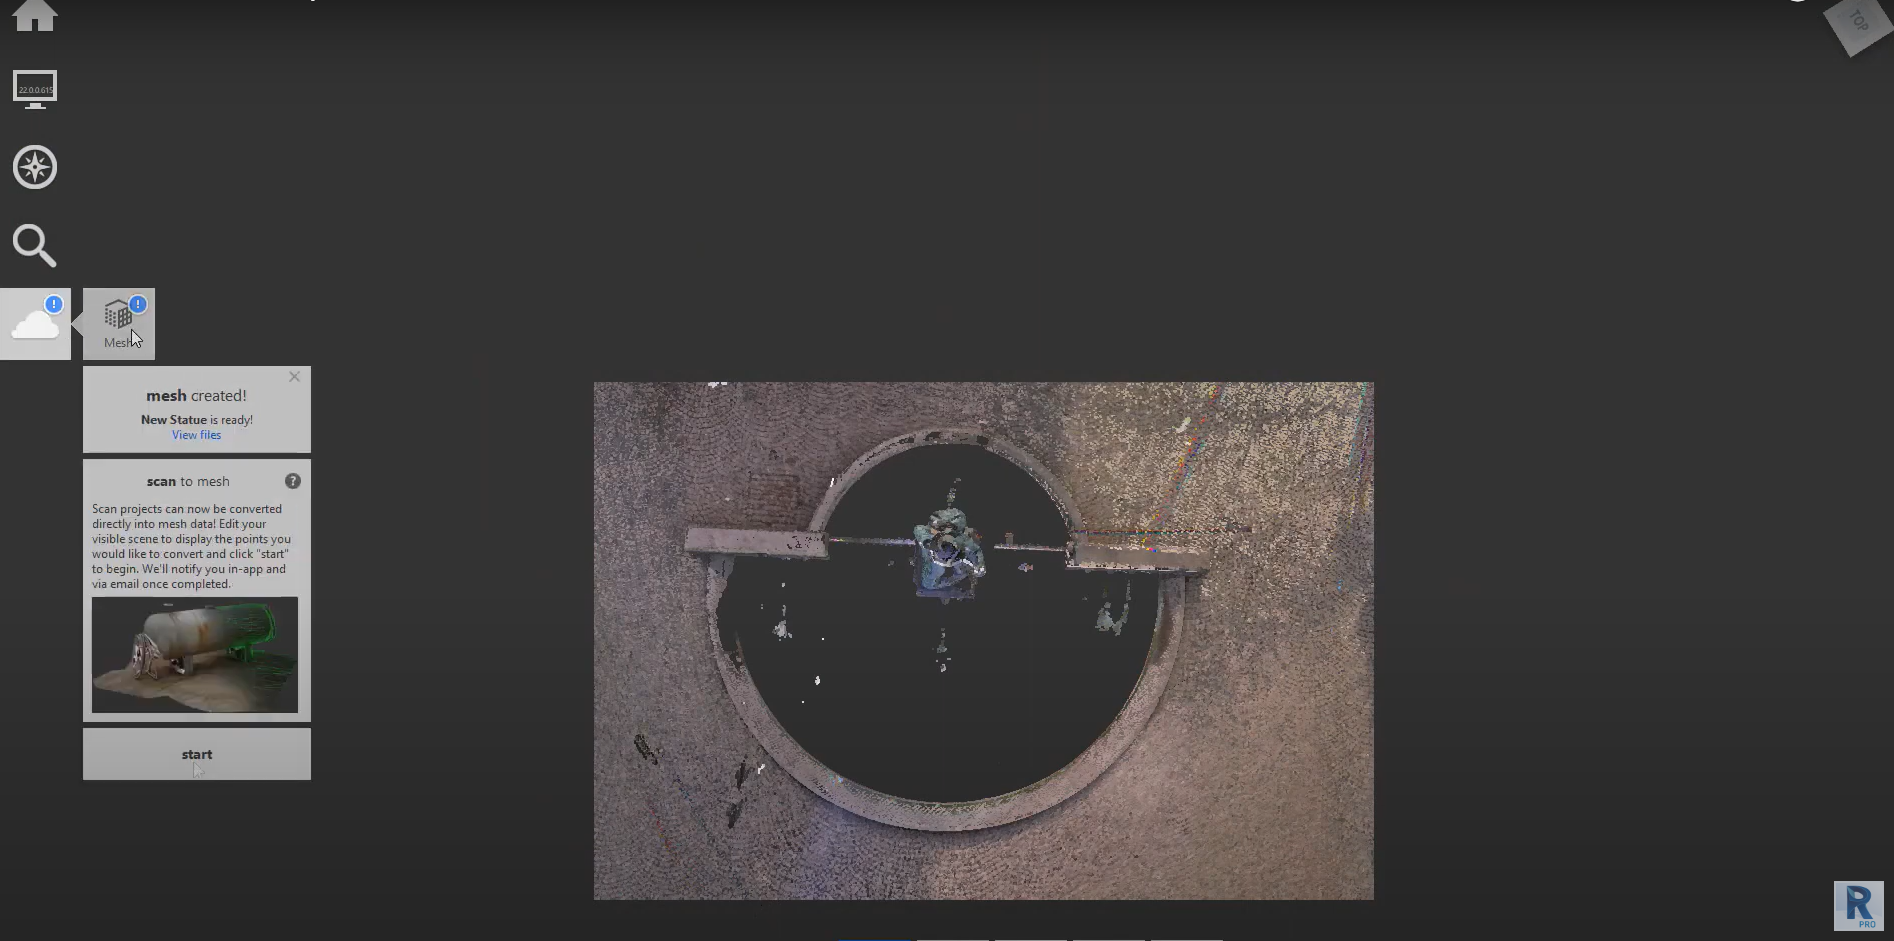
\includegraphics[width= 0.9\textwidth]{Figures/Mesh option.PNG}
  \caption[Portion of selectded Point Cloud]{Picture of selected portion of point cloud }
\end{figure}
\noindent \textbf{Final step}: Meshed point cloud in Autodesk ReCap pro
\begin{figure}[H]
  \centering
  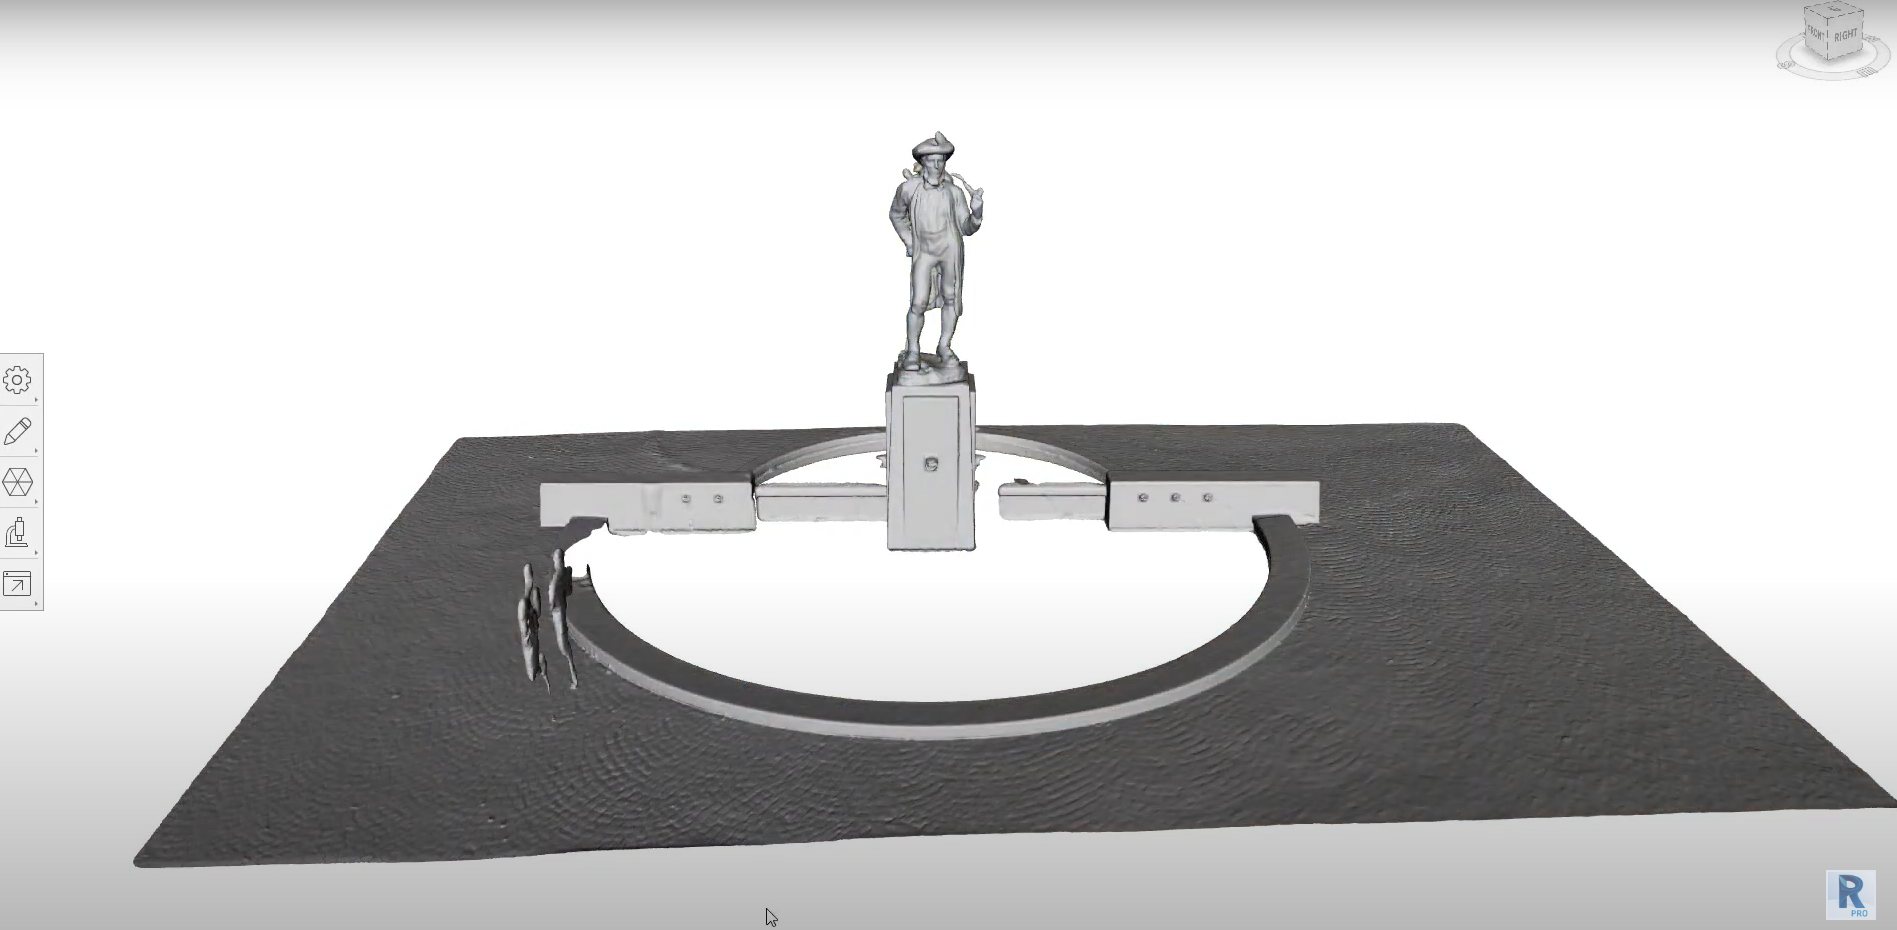
\includegraphics[width= 0.9\textwidth]{Figures/Finalmesh.PNG}
  \caption[Final Mesh]{Final Mesh}
\end{figure}
\noindent Now by this model, architectures can make a CAD model for 3D reconstruction.
\section{Point Cloud of Scanned Hallway}
After processing the scanned data with Agisoft Metashape software we get point cloud of hallway which showed in Figure \ref{fig:Hallway pointcloud}.

\begin{figure}[H]
  \centering
  \subfloat[Hallway point cloud from front view.]{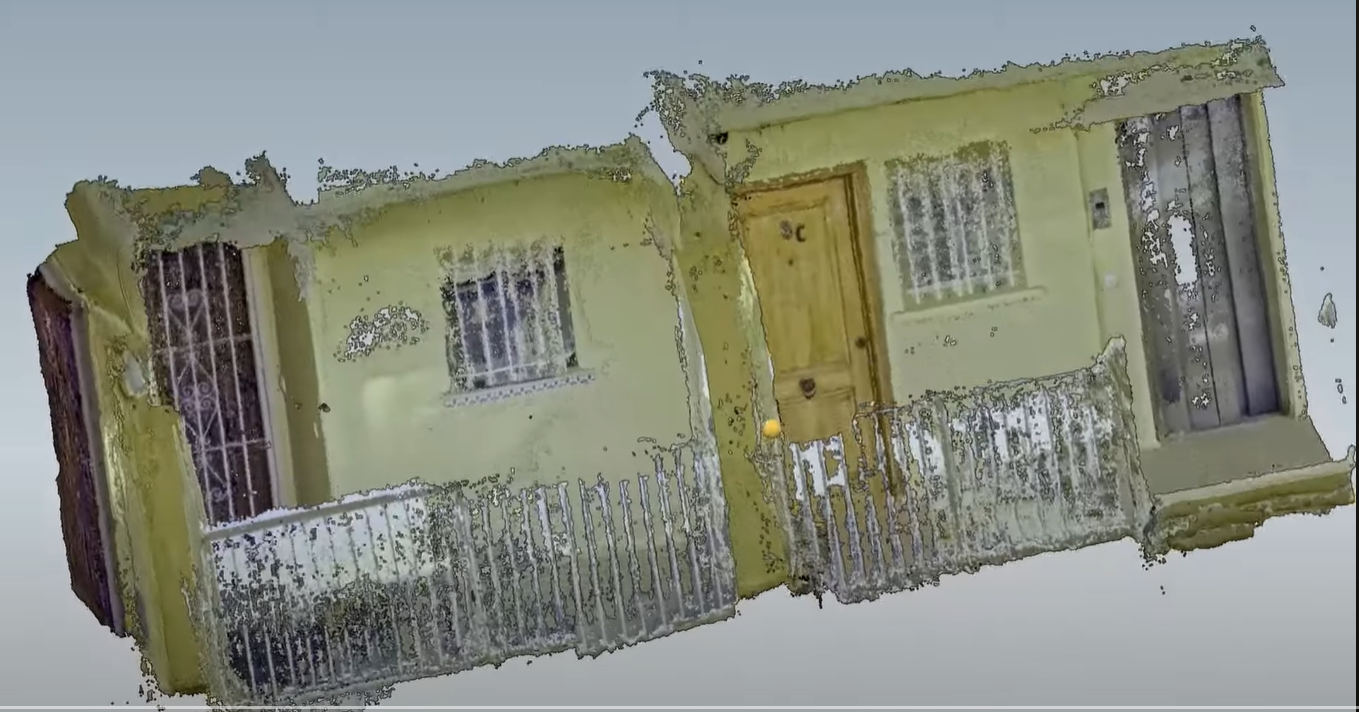
\includegraphics[width=0.9\textwidth]{Figures/hallscan.PNG}\label{fig:hallscan}}
  \hfill
  \subfloat[Hallway entrance point cloud visualized in Blender software.]{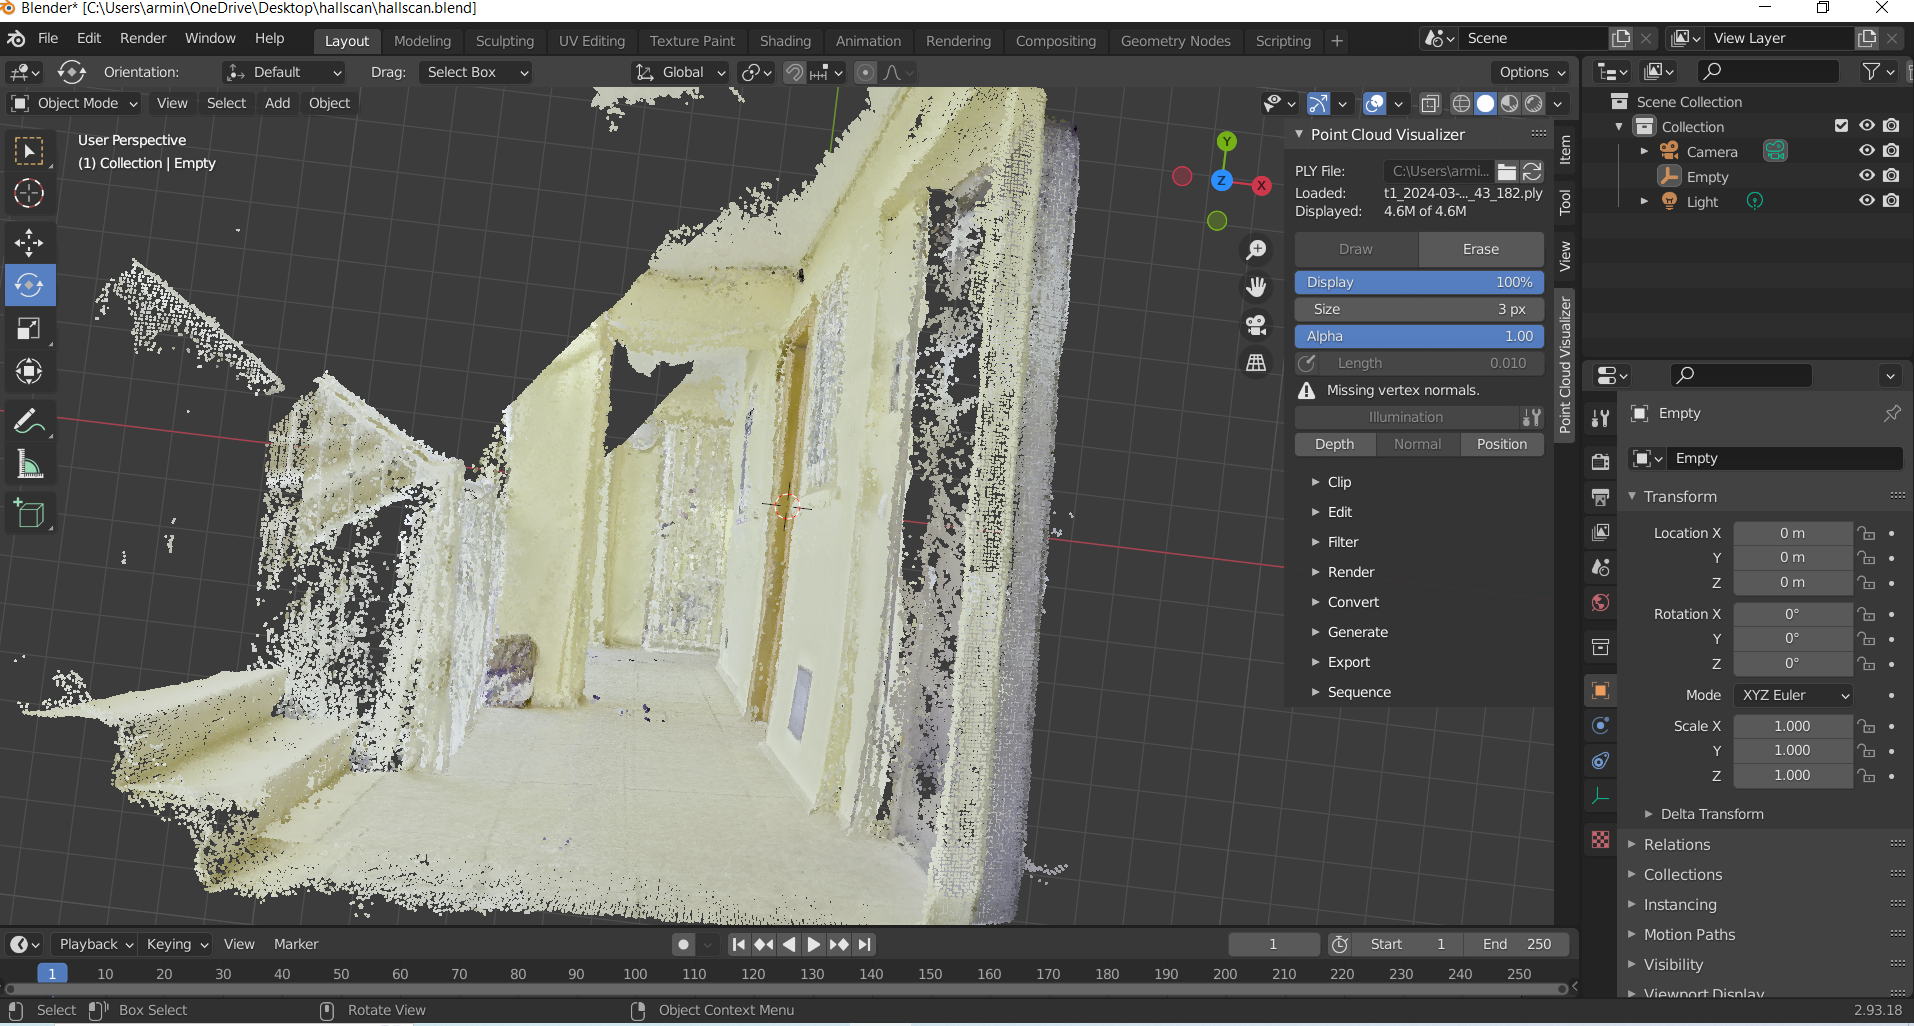
\includegraphics[width=0.9\textwidth]{Figures/Blender file of corridoor scan.PNG}\label{fig:Hallway point cloud in Blender}}
  \hfill
  \subfloat[Hallway point cloud from closer view.]{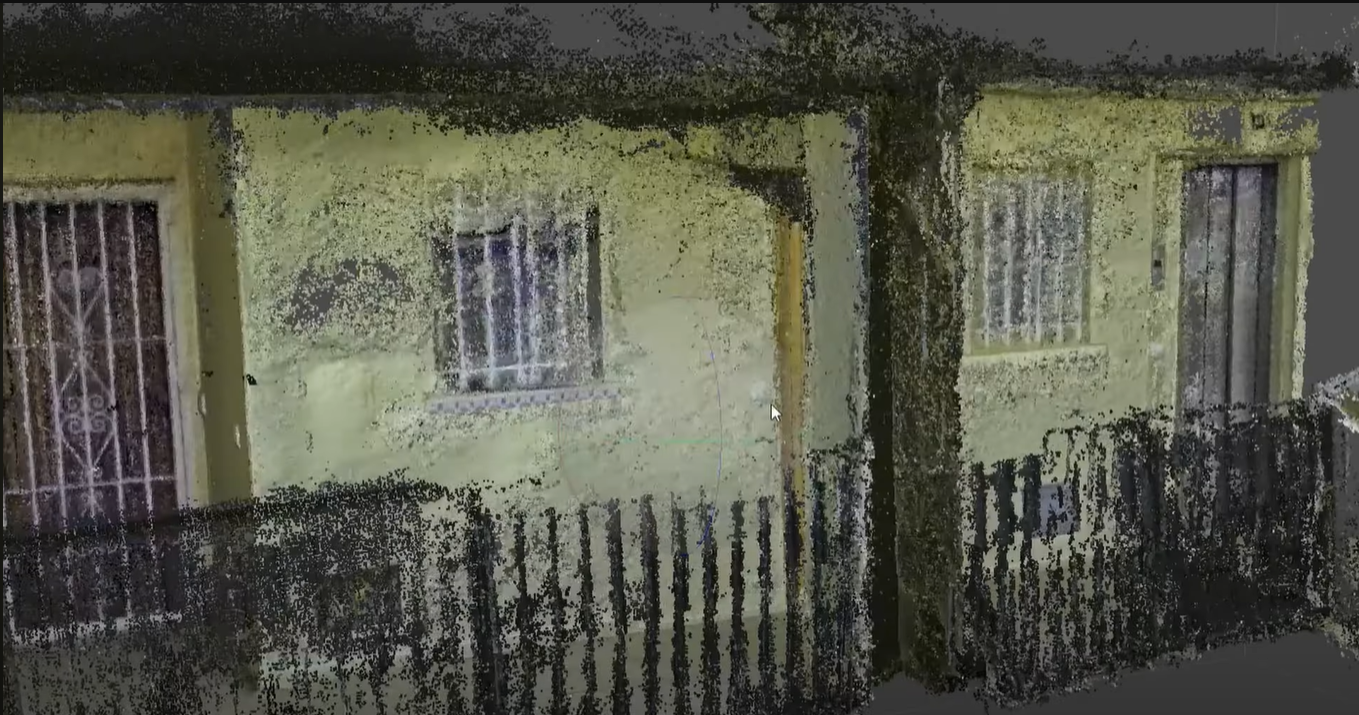
\includegraphics[width=0.8\textwidth]{Figures/hallscan1.PNG}\label{fig:Hallway point cloud from close view}}
  
  \caption[Hallway point cloud from closer view]{Figure (a) shows the point cloud from front view, figure (b) shows the start of scanning location and its point cloud, and figure (c) shows the point cloud from closer view.}
\label{fig:Hallway pointcloud}
\end{figure}

\noindent Next step is adding mesh to the point cloud with Cloud Compare. As it is shown in Figure \ref{fig:Hallway with Mesh} the mesh is added to the point cloud of hallway.
\begin{figure}[H]
  \centering
  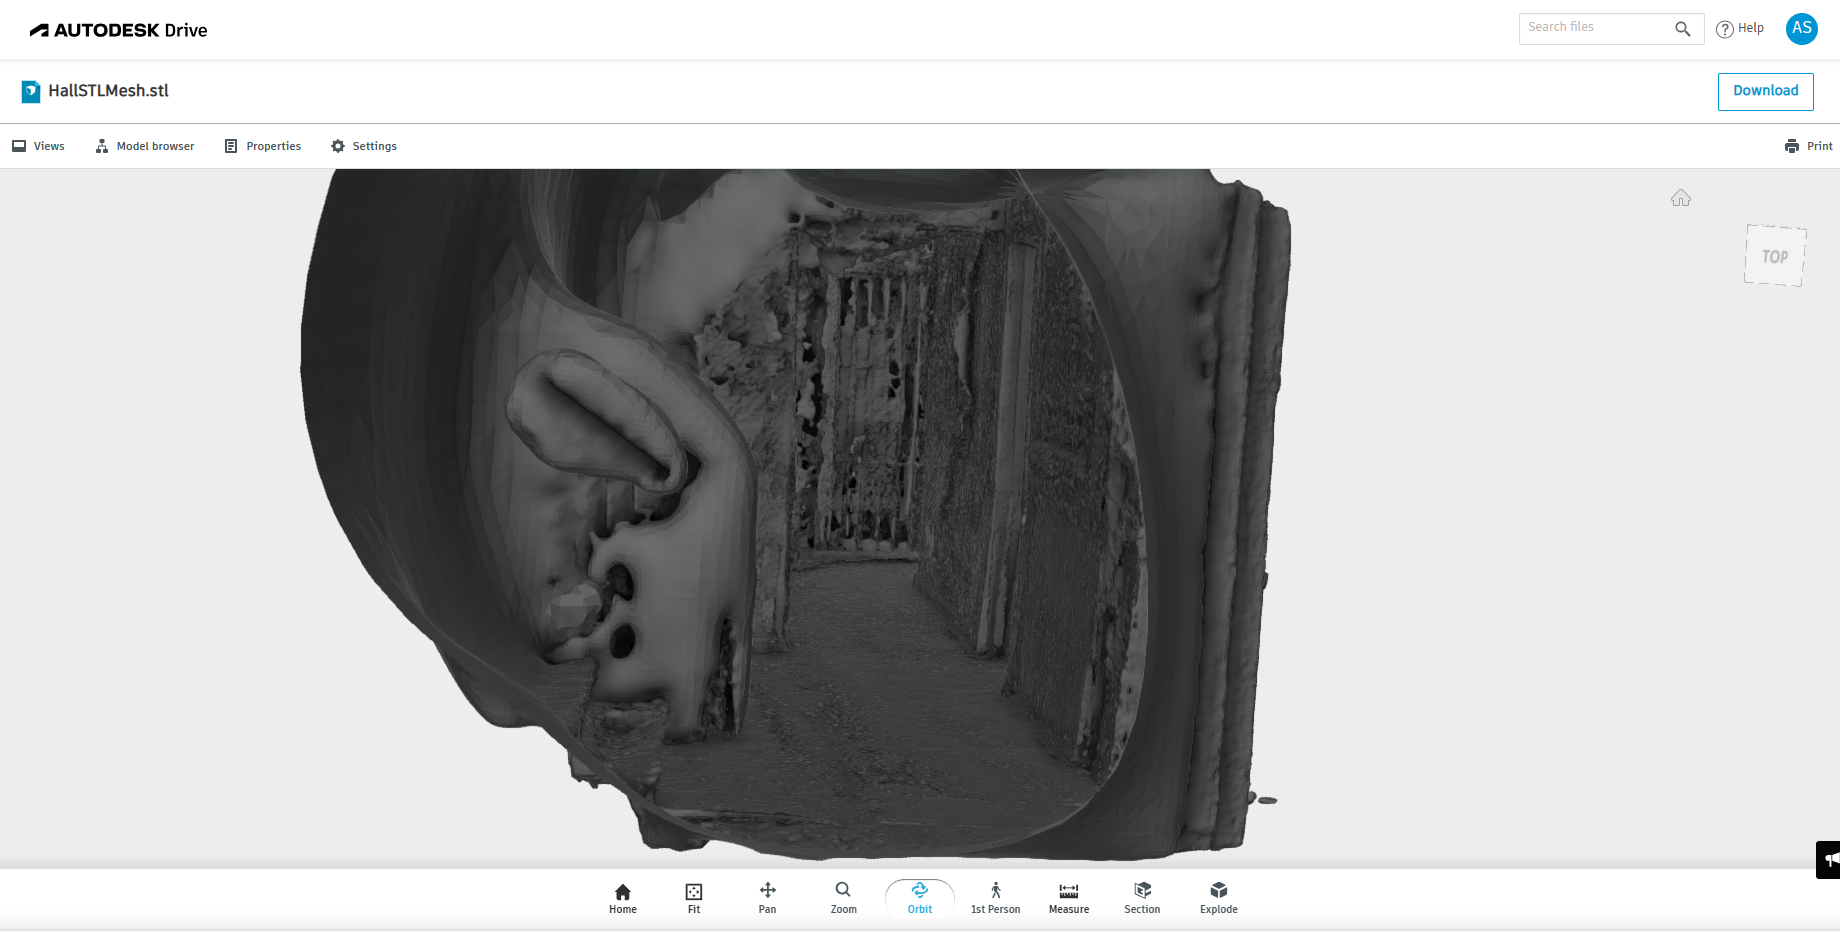
\includegraphics[width= 1.0\textwidth]{Figures/Meshhall.PNG}
  \caption[Picture of Meshed Hallway]{Picture of hallway with mesh}
  \label{fig:Hallway with Mesh}
\end{figure}
Now my meshed hallway is ready to be imported to the Coppeliasim software for simulation, after import I decided to simulate behaviour of an UGV (Unmanned Ground Vehicle) called "Pioneer p3dx" with two different algorithms and environment. The environment is shown in Figure
\ref{fig:Path visualization of pioneer p3dx}.

\begin{figure}[H]
  \centering
  \subfloat[Virtual indoor environment in CoppeliaSim]{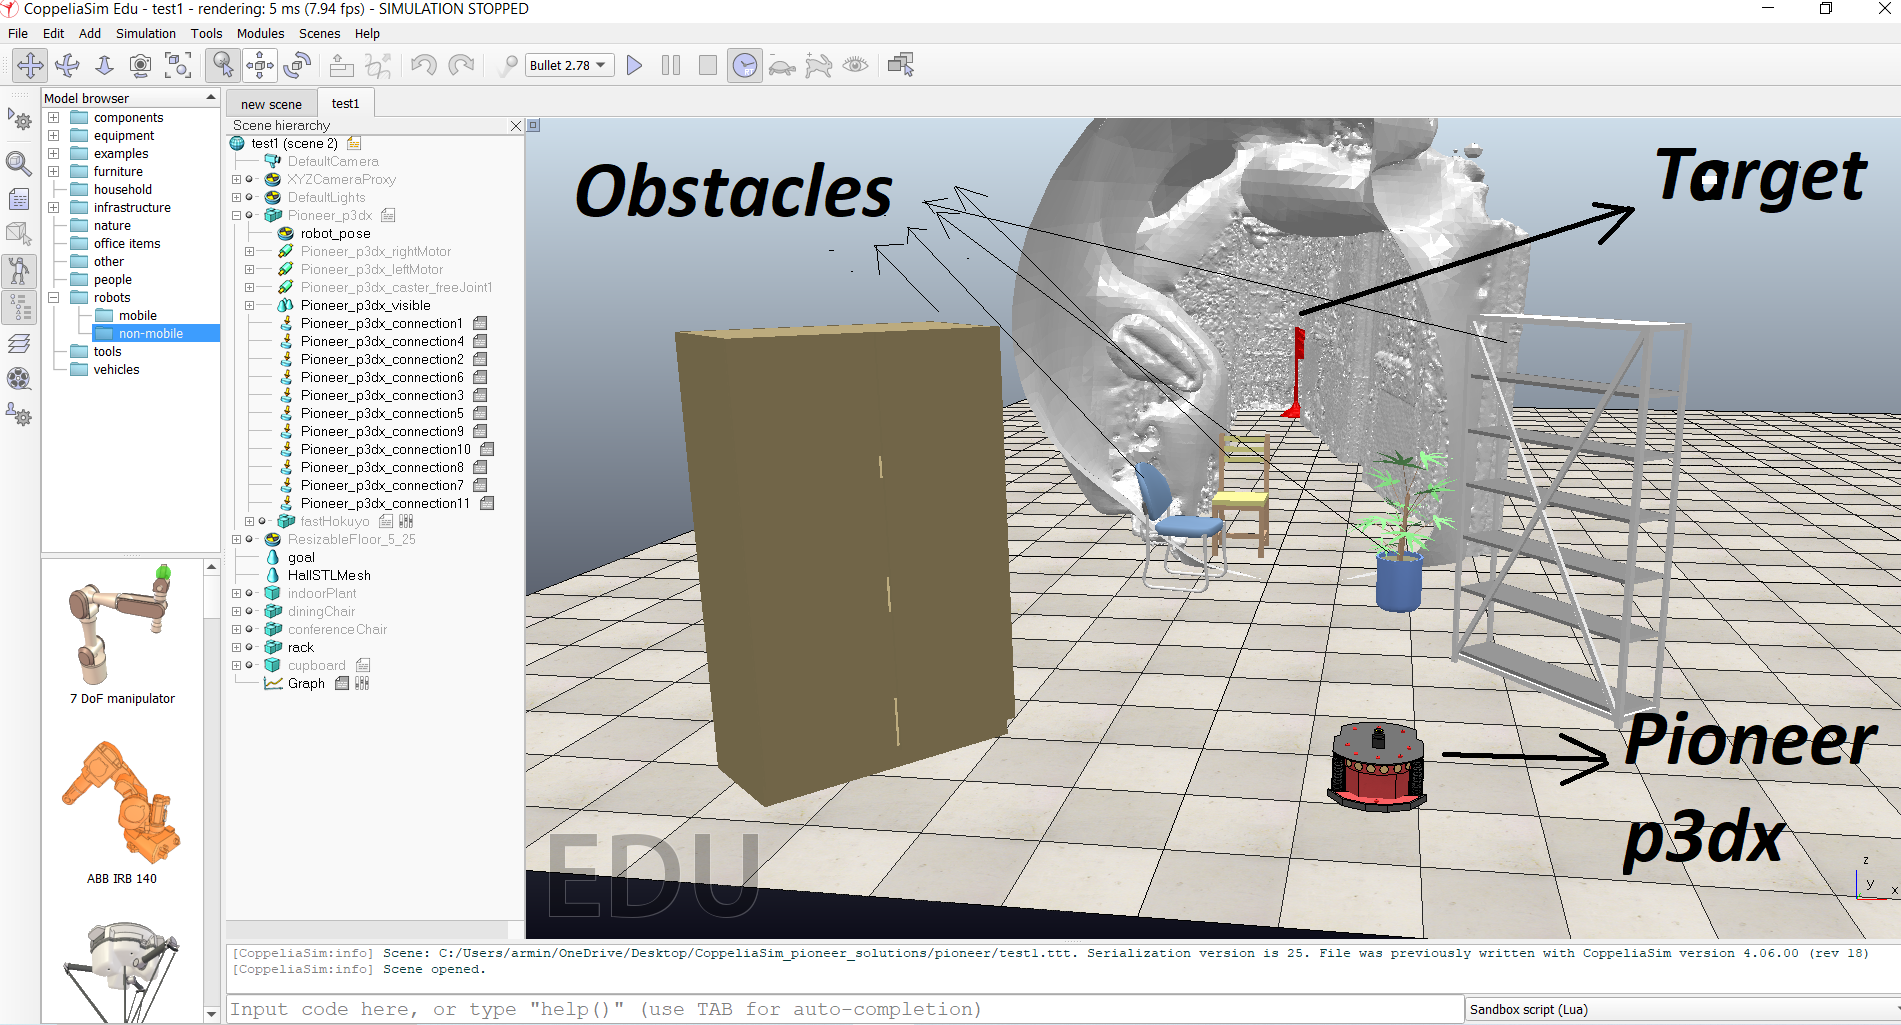
\includegraphics[width=0.9\textwidth]{Figures/Indoor environment.PNG}\label{fig:CoppeliaSim Virtual Environment}}
  \hfill
  \subfloat[Coordination of virtual environment]{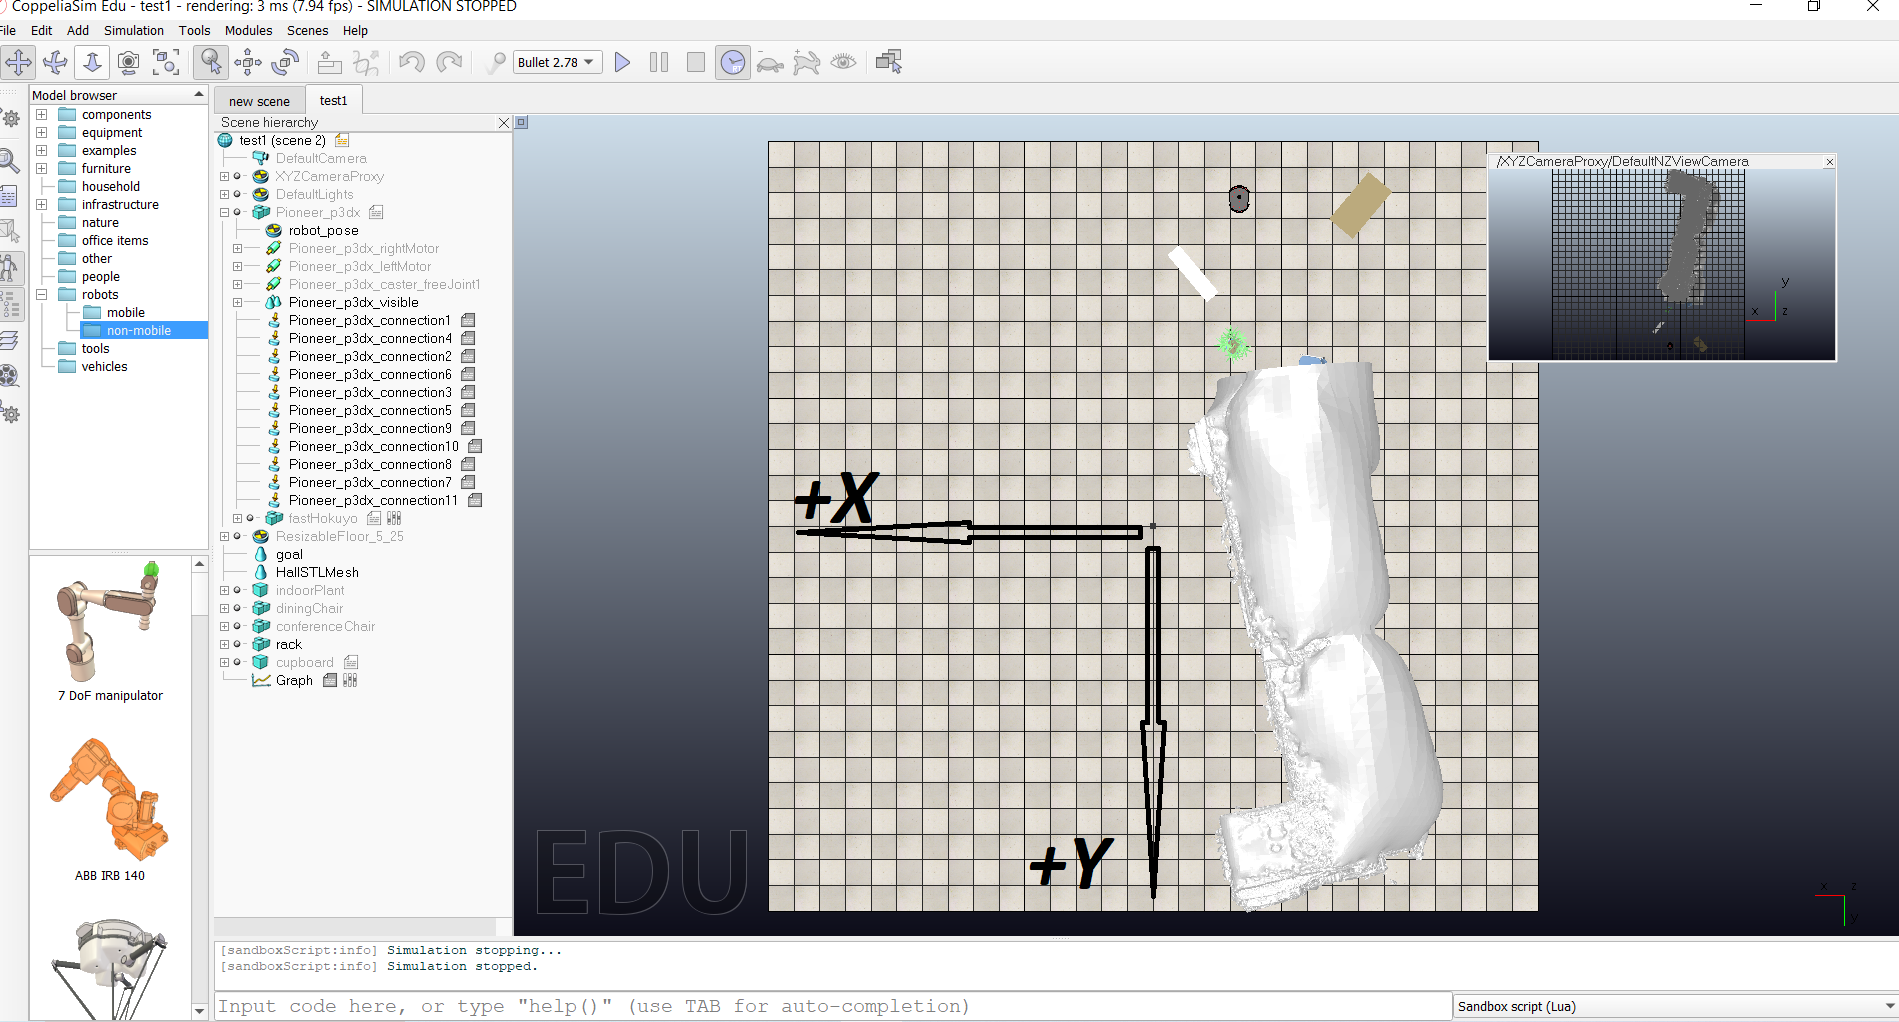
\includegraphics[width=0.7\textwidth]{Figures/Coordinate in Copppelia.PNG}\label{fig:CoppeliaSim Coordination}}
  \hfill
  \subfloat[Path and velocity direction graph of Pioneer p3dx after goal tracking]{\includegraphics[width=1\textwidth]{Figures/Path and Velocity direction graph.PNG}\label{fig:Path visualization of pioneer p3dx}}
  
  \caption[Simulation in CoppeliaSim]{Figure (a) Shows a virtual environment based on the imported mesh , figure (b) shows coordination in the CoppeliaSim, and figure (c) shows path and velocity direction of the Pioneer p3dx.}
\label{fig:Path visualization of pioneer p3dx}
\end{figure}



\section{Point Cloud in Shipbuilding Sector}

First it was planned to scan a ship with 360 degree camera for point cloud generation, but due to confidentiality of projects, it was not possible.So I decided to find a Pre-made point cloud of a ship Called SY Carola from Scottish Maritime Museum. SY Carola is possibly the world's oldest seagoing steam yacht. Scott and Sons of Bowling built it in 1898 at their shipyard on the Clyde River's north bank. Carola is 70 feet long and made of steel, with teak decking and a deckhouse. She presently has two masts.
Carola, built for personal use by the shipbuilder's family, served as a yacht during the summer months and, when not in use by the family, took groups of senior yard staff on Clyde excursions. In the winter, it would have been used as a tender and tug at the shipyard.By 1964, it had been sold to a private owner before being purchased by a Sussex corporation in 1981 and converted into corporate hospitality.
Carola joined the Scottish Maritime Museum's collection in 1994.
The model was developed as part of the 'Scanning The Horizon' 3D digitisation project\cite{Carolaship}. In Figure \ref{fig:SY Carola point cloud} the Carola point cloud is shown. 

\begin{figure}[H]
  \centering
  \includegraphics[width= 0.9\textwidth]{Figures/Crolaship.PNG}
  \caption[Picture of Visualized SY Carola Point Cloud]{Picture of SY Carola point cloud} \cite{Carolaship}
   \label{fig:SY Carola point cloud}
\end{figure}
\noindent After that I tried to import the point cloud to the CoppeliaSim for robot simulation on the deck but, the imported point cloud was black and not suitable as a virtual environment, although the the point cloud was detectable, collidable and measurable by the virtual robot. In figure \ref{fig:SY Carola point cloud} the imported point cloud to the CoppeliaSim is shown. 
\begin{figure}[H]
  \centering
  \includegraphics[width= 0.8\textwidth]{Figures/ship point clould in Coppeliasim.PNG}
  \caption[Picture of SY Carola Point Cloud in CoppeliaSim]{Picture of SY Carola point cloud in CoppeliaSim}
   \label{fig:Carola point cloud in CoppeliaSim}
\end{figure}
\noindent So then I tried to use mesh of Carola ship to import to the CoppeliaSim. As it is shown in Figure \ref{fig:Mesh of SY Carola in Autodesk}. 
\begin{figure}[H]
  \centering
  \includegraphics[width= 0.9\textwidth]{Figures/Carola mesh.PNG}
  \caption[Mesh of SY Carola in Autodesk]{Mesh of SY Carola in Autodesk}
   \label{fig:Mesh of SY Carola in Autodesk}
\end{figure}

\noindent But due to less-complexity of Carola,s deck obstacles for robot simulation, I selected a ship with complex deck design.The imported mesh is shown in Figure \ref{fig:Mesh of A Ship in CoppeliaSim}. 
\begin{figure}[H]
  \centering
  \includegraphics[width= 1.0\textwidth]{Figures/CoppeliaMesh.PNG}
  \caption[Mesh of A Ship in CoppeliaSim]{Mesh of A Ship in CoppeliaSim}
   \label{fig:Mesh of A Ship in CoppeliaSim}
\end{figure}



\section{Qualitative and Quantitative Results}
\noindent In this section I simulated Pioneer 3dx robot in my virtual environment with two prefabricated algorithms called: potential field and Vector Field Histogram Plus(VFH+). One of the virtual environments is an indoor place (scanned hall) and another one is an
outdoor environment (ship model). Two types of qualitative and quantitative results have been compared and investigated.
  
\subsection{Simulation With Pioneer 3dx Based on the Potential Field Method in a Scanned Hall Mesh (Indoor Environment) }
\noindent As you can see in the Figure \ref{fig:Indoor environment with scanned hall mesh} the robot is located between obstacles with different sizes and locations. The goal is at the end of scanned hall in right side which is source of attractive force in the environment.   
\begin{figure}[H]
  \centering
  \includegraphics[width= 0.6\textwidth]{Figures/1.PNG}
  \caption[Indoor environment with scanned hall mesh]{Indoor environment with scanned hall mesh} 
   \label{fig:Indoor environment with scanned hall mesh}
\end{figure}

\noindent In the Figure \ref{fig:Obstacles in the scene without hidden scanned hall mesh} it is shown the environment with hidden hall mesh to be clear about the place of obstacles and goal.  

\begin{figure}[H]
  \centering
  \includegraphics[width= 0.6\textwidth]{Figures/2.PNG}
  \caption[Obstacles in the scene without hidden scanned hall mesh]{Obstacles in the Scene without hidden scanned hall mesh}
   \label{fig:Obstacles in the scene without hidden scanned hall mesh}
\end{figure}
After testing the robot in different environment arrangement, it found that in the following arrangement the robot will be trapped: 


\begin{itemize}
      \item  \textbf{ U-shape Obstacles or Concave Obstacles: }\\
      The robot can be trapped in u-shape or concave geometries due to local minimum specifically when the robot is far from the goal.   
      A polygon is convex if its inner angles are all fewer than 180 degrees. If one or more internal angles exceed 180 degrees, the polygon is non-convex (or concave). In Figure \ref{fig:Concave polygon and U-shape Obstacle} shown the two obstacles with repulsive forces around, one is u-shape and another one is a concave polygon which the possibility of trapping the robot is high. 
\begin{figure}[H]
  \centering
  \includegraphics[width= 0.8\textwidth]{Figures/Concave polygon and U-shape.png}
  \caption[Concave polygon and U-shape Obstacle]{Concave polygon and U-shape Obstacle}
   \label{fig:Concave polygon and U-shape Obstacle}
\end{figure}
       \item  \textbf{ Oscillatory Behavior Between Obstacles: }\\
       In potential field method , there is a problem of oscillatory behavior of robot when the step size is too large. This issue happens when repulsive forces can be significantly higher than the attractive one which can cause the robot not to pass between obstacles even if physically could be possible. In Figure \ref{fig:Oscillatory Behavior} it is shown the situation that the robot stuck between a plant and hall structure.  
\begin{figure}[H]
  \centering
  \includegraphics[width= 0.8\textwidth]{Figures/Oscillatory stuck.PNG}
  \caption[Oscillatory Behavior]{Oscillatory Behavior}
   \label{fig:Oscillatory Behavior}
\end{figure}

       
       \item  \textbf{ Crowded Obstacles : }\\
       In crowded areas, potential field approaches can cause the robot to become trapped. This is typically related to the formation of local minima in the potential field. As it is shown in the Figure \ref{fig:Crowd Obstacles} the summation of repulsive forces from obstacles are stronger than attractive force so the robot will stuck even if physically possible to pass the obstacles. 
\begin{figure}[H]
  \centering
  \includegraphics[width= 0.9\textwidth]{Figures/Crowd obstacles.png}
  \caption[Crowd Obstacles]{Crowd Obstacles}
   \label{fig:Crowd Obstacles}
\end{figure}

       
       \item  \textbf{ Less Detectable Obstacles: }\\
       The Artificial Potential Field (APF) method for robot path planning use a laser scanner to detect impediments. The robot perceives these impediments as sources of repulsive forces and attempts to maneuver around them. However, if the impediments are less noticeable or smaller than the threshold specified in the robot's programming, they may not be recognized as barriers. If a barrier is too small or not reflecting enough, the laser scanner may not detect it at all. This means that the robot will not recognize the impediment and may collide with it. Even if a little barrier is recognized, its repulsive force may not be sufficient to deflect the robot, particularly if the robot is moving quickly. As an example in our environment, legs of chairs are less detectable obstacles, an shown in Figure \ref{fig:Chair legs as less detectable obstacles}.   
\begin{figure}[H]
  \centering
  \includegraphics[width= 0.7\textwidth]{Figures/Chair legs.PNG}
  \caption[Chair legs as less detectable obstacles]{Chair legs as less detectable obstacles}
   \label{fig:Chair legs as less detectable obstacles}
\end{figure}

       \item  \textbf{ Height of Obstacles Which are Lower or Higher Than Laser Sensor Height : }\\
       The Artificial Potential Field (APF) method for robot path planning use a laser scanner to detect impediments. However, obstructions that are higher or lower than the laser scanner level can be difficult to navigate. If an obstacle is higher than the laser scanner's level, the scanner may be unable to identify it completely, especially if the barrier is close to the robot. This could result in erroneous mapping of the environment and possible collisions. Similarly, if an obstacle is below the level of the laser scanner, it may not be recognized at all. This is especially problematic for minor objects on the ground, which might lead the robot to trip or become trapped. A schematic view of this issue shown in Figure 
       \ref{fig:Higher and lower obstacles height than robot laser level}. 

\begin{figure}[H]
  \centering
  \includegraphics[width= 0.9\textwidth]{Figures/Laser level.png}
  \caption[Higher and lower obstacles height than robot laser level]{Higher and lower obstacles height than robot laser level}
   \label{fig:Higher and lower obstacles height than robot laser level}
\end{figure}
       
\end{itemize}




\subsection{Simulation With Pioneer 3dx Based on the Potential Field Method on the Deck of a Ship (Outdoor Environment) }
\noindent After importing the mesh or CAD model of a ship to the CoppeliaSim Software, I simulated a marine fire fighting operation with robot. Some items added to the scene to be more realistic like industrial robot, virtual fire and a flag. In Figure 
\ref{fig:Robot simulation on the deck of a ship for a short-range firefighting operation} it is shown the robot operation on the deck. This robot can autonomously navigate toward fire source if it does not trap. simulation has been done by adding more obstacles in the way of robot, or putting the robot back of an obstacle ,and it is seen that the likelihood of robot trapping is too much.  So it looks like potential field is better for short-range operation with less congested environment arrangement. \\
\begin{figure}[H]
  \centering
  \includegraphics[width= 0.9\textwidth]{Figures/shipAPFSIM.PNG}
  \caption[Robot simulation on the deck of a ship for a short-range firefighting operation]{Robot simulation on the deck of a ship for a short-range firefighting operation}
   \label{fig:Robot simulation on the deck of a ship for a short-range firefighting operation}
\end{figure}

\subsection{Simulation with Vector Field Histogram Plus (VFH+) Method in an virtual Outdoor Environment with terrain) }

In this environment, robot surrounded by trees, scanned hall and terrains. Type of the terrains were implemented in this simulation was not complex terrains with lots of ups and downs. In Figure \ref{fig:Outdoor Environment for VFH+ Algorithm Simulation} the environment has been shown. 
\begin{figure}[H]
  \centering
  \includegraphics[width= 1.0\textwidth]{Figures/VFH+TERRAIN.PNG}
  \caption[Outdoor Environment for VFH+ Algorithm Simulation]{Outdoor Environment for VFH+ Algorithm Simulation}
   \label{fig:Outdoor Environment for VFH+ Algorithm Simulation}
\end{figure}
\noindent In this arrangement the robot located left side of hall and goal located in the right side of the hall. First the robot try to reduce captured data by making a map of occupied cells by defining a 2d cell histogram. Then based on the likelihoods of occupied cells in the active region the robot try to make a 1d polar histogram and in this process the size of the robot is also take into account. 
To be familiar with size and some other features of this robot we can see the Figure \ref{fig:Robot Features}. 
\begin{figure}[H]
  \centering
  \includegraphics[width= 0.6\textwidth]{Figures/robot features.PNG}
  \caption[Robot Features]{Robot Features}
   \label{fig:Robot Features} \cite{PF}
\end{figure}

\noindent The features are b (distance from one wheel to the robot center line), e (off-kinematic control point), wheel radius, stop distance, safety distance and the amounts are: \\
\begin{align*}
\text{wheel\_radius} &= \frac{0.195}{2} \\
b &= 0.1655 \\
\text{stop\_distance} &= 0.2 \\
\text{safety\_distance} &= 0.55 \\
e &= 0.3\\
\text{scan\_angle} &= \text{math.rad(sim.getUserParameter(hokuyo,'scanAngle'))} \\
\text{cell\_size} &= 0.1 \\
\text{window\_size} &= 2 \times \text{sim.getUserParameter(hokuyo,'maxScanDistance')} \\
\text{sector\_angle} &= \text{math.rad(5)} \\
\text{wide\_sector\_width} &= 5 \\
\tau_{\text{low}} &= 500 \\
\tau_{\text{high}} &= 2000 \\
\text{target\_weight} &= 3 \\
\text{previous\_weight} &= 2 \\
\text{current\_weight} &= 1
\end{align*}
\noindent After making polar histogram, robot uses from two threshold to decide if a sector was occupied or not. If bars in polar histogram are higher than a high threshold then they concluded as occupied means 1  and if bars are lower than a low threshold so they are free mean zero and otherwise the bars in between use as previous iteration value. Then based on the minimum turning radius and kinematic constrains robot decide to mask parts of histogram. After masking parts of binary histogram wide and narrow valleys remains for robot to follow. It is clear that narrow passages can not be more optimised as a route by the robot as the closest path to the goal. But wide valleys can be optimised by 3 items of target weight, previous orientation's weight and robot's orientation weight to minimise the cost function. \\
\noindent To fine-tune the three terms in the cost function formula \eqref{eqn:Cost Function} I tested the variation of target weight (fisrt term) versus time to reach the goal to find the optimised target weight for the robot based on the shortest time. I fixed all parameters except target weight. The results of simulation shown on the Table \ref{table:Variation of Target Weight Versus Time to Reach the Goal}. All the routes passed by robot were the same pattern (here means almost the same distance) in all variations of target weight. The picture of the yellow path is shown from top view in the Figure \ref{fig:Robot Path to Goal}. 

\begin{figure}[H]
  \centering
  \includegraphics[width= 0.6\textwidth]{Figures/Tw-03.PNG}
  \caption[Robot Path to Goal]{Robot Path to Goal}
   \label{fig:Robot Path to Goal} 
\end{figure}

\begin{table}[ht!]
\centering
    \begin{tabular}{ m{3cm} m{5cm} m{5cm} } 
    \toprule
    \toprule
    \textbf{Target Weight} & \textbf{Reach to Goal or Not} & \textbf{Time to Reach Goal (s)} \\
    \midrule
    1      & 0       &    \\[1.3ex]
    2       & 100    & 77   \\[1.3ex]
    3      & 100     & 76   \\[1.3ex]
    4      & 100     & 91   \\[1.3ex]
    5      & 100    & 91   \\[1.3ex]
    6     & 100     & 104     \\[1.3ex]
    7     & 100     & 75     \\[1.3ex]
    8     & 100     & 75   \\[1.3ex]
    9     & 0       &    \\[1.3ex]
    \bottomrule
    \bottomrule
\end{tabular}
\caption[Variation of Target Weight Versus Time to Reach the Goal]{Table of variation of target weight versus time to reach the goal are based on the same pattern of path. Target weight tested from 1 to 9 numbers, the reach to goal is based on the zero (not reach the goal)and one (reach the goal), the time to reach goal is based on the seconds. }
\label{table:Variation of Target Weight Versus Time to Reach the Goal}
\end{table} 
\noindent With Target Weight (TW) 1 the robot lost in the environment and could not find the path toward goal, seems the low amount of this item cause orientation loss. With TW of 2,the robot passed the obstacles and reached the goal in 77 seconds. In TW of 3,took 76 seconds and in TW of 4 and 5 took 91 seconds for robot to reach the goal, the reason was temporary stuck of robot to the bumps on the terrain due to the structural design of Pionner 3dx robot. In target weight 6, robot had the longest time of stuck after terrain bumps. Finally target weight 7 was the shortest time to reach the goal and the optimised one with 75 seconds. A graph of variation of target weight versus time to reach goal is shown in Figure \ref{fig:Graph of Variation of Target Weight Versus Time to Reach the Goal}. 
\begin{figure}[H]
  \centering
  \includegraphics[width= 1.0\textwidth]{Figures/Target vs Time.PNG}
  \caption[Graph of Variation of Target Weight Versus Time to Reach the Goal ]{Graph of Variation of Target Weight Versus Time to Reach the Goal}
   \label{fig:Graph of Variation of Target Weight Versus Time to Reach the Goal} 
\end{figure}


\subsection{Simulation with Vector Field Histogram Plus Method on the deck of a ship with Many obstacles) }
In this environment, robot surrounded by obstacles imported on the deck of a ship to making a complex path for robot to plan the target. In figure \ref{fig:Virtual Robot Simulation on the Deck of a Ship with VFH+ Algorithm} the robot mission on the deck is extinguishing the fire on the shortest time on the other side of the ship to prevent catastrophic consequences of spreading fire. And this simulation proofs the ability of autonomous path planning mobile robots for safer marine operation. 
\begin{figure}[H]
  \centering
  \includegraphics[width= 1.0\textwidth]{Figures/VFH+SHIP.PNG}
  \caption[Virtual Robot Simulation on the Deck of a Ship with VFH+ Algorithm ]{Virtual Robot Simulation on the Deck of a Ship with VFH+ Algorithm}
   \label{fig:Virtual Robot Simulation on the Deck of a Ship with VFH+ Algorithm} 
\end{figure}
\noindent I tested the variation of target weight versus time to reach the fire to find the optimised target weight for the robot based on the shortest time on the deck of a ship. I took constant all parameters except target weight. The results of the simulation shown on the Table \ref{table:Variation of Target Weight Versus Time to Reach the Goal on the Ship}. The picture of the yellow path shown from top view in the Figure \ref{fig:Robot Path with Target Weight of 6} is for target weight of 6 and in Figure \ref{fig:Robot Path with Target Weight of 7} is for target weight of 7. During the testing of different target weight versus time which it is important to mention that the pattern change of robot's path from TW 6 to 7, actually route reduced to reach the goal. And in TW 9, the robot stuck in the turn which is close to industrial robot. 

\begin{figure}[h]
    \centering
    \begin{minipage}{1.0\textwidth}
        \centering
        \includegraphics[width=0.9\textwidth]{Figures/TW-6.PNG} % first figure itself
        \caption{Robot Path with Target Weight of 6}
        \label{fig:Robot Path with Target Weight of 6}    
    \end{minipage}\hfill
    \begin{minipage}{1.0\textwidth}
        \centering
        \includegraphics[width=0.9\textwidth]{Figures/TW-7.PNG} 
        \caption{Robot Path with Target Weight of 7} 
        \label{fig:Robot Path with Target Weight of 7}
    \end{minipage}
\end{figure}

\begin{table}[ht!]
\centering
    \begin{tabular}{ m{3cm} m{5cm} m{5cm} } 
    \toprule
    \toprule
    \textbf{Target Weight} & \textbf{Reach to Goal or Not} & \textbf{Time to Reach Goal (s)} \\
    \midrule
    1      & 0       &    \\[1.3ex]
    2       & 0    &    \\[1.3ex]
    3      & 100     & 131   \\[1.3ex]
    4      & 100     & 133   \\[1.3ex]
    5      & 100    & 133   \\[1.3ex]
    6     & 100     & 132     \\[1.3ex]
    7     & 100     & 110     \\[1.3ex]
    8     & 100     & 110   \\[1.3ex]
    9     & 100       & 120   \\[1.3ex]
    10     & 100       & 141   \\[1.3ex]
    11     & 100       & 131   \\[1.3ex]
    12     & 100       & 117   \\[1.3ex]
    13     & 100       & 115   \\[1.3ex]
    14     & 100       & 115   \\[1.3ex]
    15     & 100       &117    \\[1.3ex]
   16     & 100       &117    \\[1.3ex]
    \bottomrule
    \bottomrule
\end{tabular}
\caption[Variation of Target Weight Versus Time to Reach the fire on a Ship's Deck]{Table of variation of target weight versus time to reach the fire. The path of the robot will be shorter by changing the Target Weight from 6 to 7. Target weight tested from 1 to 16 numbers, the reach to goal is based on the zero (not reach the goal)and one (reach the goal), the time to reach goal is based on the seconds. }
\label{table:Variation of Target Weight Versus Time to Reach the Goal on the Ship}
\end{table} 

\noindent In another simulation scenario, I considered the target weight and robot's direction weight constant as 7 and 1 consecutively and changed the Wp (previous direction weight) and checked the goal reach-ability in a specific time and the results is in the table \ref{table:Variation of Previous Direction Weight Versus Time to Reach the Goal on the Ship}. In Wp 7, the robot will be stuck and cannot move anymore. 

\begin{table}[ht!]
\centering
    \begin{tabular}{ m{3cm} m{5cm} m{5cm} } 
    \toprule
    \toprule
    \textbf{Previous Direction Weight} & \textbf{Reach to Goal or Not} & \textbf{Time to Reach Goal (s)} \\
    \midrule
    2      & 100       & 110   \\[1.3ex]
    3      & 100     & 132   \\[1.3ex]
    4      & 100     & 133   \\[1.3ex]
    5      & 100    & 132   \\[1.3ex]
    6     & 100     & 129     \\[1.3ex]
    7     & 0     &      \\[1.3ex]
 
    \bottomrule
    \bottomrule
\end{tabular}
\caption[Variation of Previous Direction Weight Versus Time to Reach the fire on a Ship's Deck]{Table of variation of previous direction weight versus time to reach the fire. Previous direction weight tested from 1 to 7 numbers, the reach to goal is based on the zero (not reach the goal)and one (reach the goal), the time to reach goal is based on the seconds. }
\label{table:Variation of Previous Direction Weight Versus Time to Reach the Goal on the Ship}
\end{table} 
\noindent In another simulation scenario, I considered the target weight and previous direction weight constant as 7 and 2 consecutively and changed the Wc (robot's direction weight) and checked the goal reach-ability in a specific time and the results is in the table \ref{table:Variation of Robot's Direction Weight Versus Time to Reach the Goal on the Ship}. In Wc 4, the robot will stuck and cannot move anymore. 

\begin{table}[ht!]
\centering
    \begin{tabular}{ m{3cm} m{5cm} m{5cm} } 
    \toprule
    \toprule
    \textbf{Robot's Direction Weight} & \textbf{Reach to Goal or Not} & \textbf{Time to Reach Goal (s)} \\
    \midrule
    2      & 100       & 137   \\[1.3ex]
    3      & 100     & 130   \\[1.3ex]
    4      & 0     &    \\[1.3ex]
    
 
    \bottomrule
    \bottomrule
\end{tabular}
\caption[Variation of Robot's Direction Weight Versus Time to Reach the fire on a Ship's Deck]{Table of variation of robot's direction weight versus time to reach the fire. Robot's direction weight tested from 2 to 4 numbers, the reach to goal is based on the zero (not reach the goal)and one (reach the goal), the time to reach goal is based on the seconds. }
\label{table:Variation of Robot's Direction Weight Versus Time to Reach the Goal on the Ship}
\end{table} 
\noindent Based on the cost function formula \eqref{eqn:Cost Function}: 
\begin{equation}
\begin{aligned}
f(c) = W_t \Delta(c,t) + W_p \Delta ( c , p) + W_c \Delta (c)
\end{aligned}
\label{eqn:Cost Function}
\end{equation} 
\\

After several experiments an optimized set of terms for both ship and out-door environment is: 
\begin{align*}
\text{target\_weight} &= 7 \\
\text{previous\_weight} &= 2 \\
\text{current\_weight} &= 1
\end{align*}
\\




\vspace{20cm}

\section{Discussion}

\noindent 1. Simulation in a captured point cloud trigger to a virtual experience of a real environment but if we wanted to use a real robot for simulation can endanger both the robot and the environment, especially in dangerous situations like fire fighting operations.\\

\noindent 2. Virtual environments enable safe testing without the threat of actual injury. Creating and maintaining actual prototypes for real-world testing can be costly. Virtual testing lowers expenses by reducing the requirement for actual prototypes during the early phases of development.\\

\noindent 3. Making design adjustments and testing findings on a real robot can take some time. Virtual environments enable engineers to iterate quickly on design and functionality, hence shortening the development cycle.\\

\noindent 4. It can be difficult to regulate all factors in the real world. Virtual navigation enables exact control over the environment and variables, enabling more detailed and controlled testing situations.\\

\noindent 5. Training operators on actual robots can be dangerous and expensive. Virtual environments offer a safe, controlled setting for training before going on to real-world tasks.  \\

\noindent 6. Collecting data on robot performance and behavior in the real world can be difficult and time intensive. Virtual environments can efficiently capture vast volumes of data, which can then be used to improve robot performance and operational protocols.\\

\noindent 7. Real-world testing necessitates actual presence, which might be restrictive. Virtual testing is accessible from anywhere, allowing teams to interact and train in many locations.\\

\noindent 8. The results showed that Robot stuck several times in potential field algorithms simulation,due to sticking of robot in local minimum, this algorithm was not comparable with VFH+, so I decide to fine tune the VHF+ parameters for different arrangements.   \\

\noindent 9. In the Vector filed histogram plus algorithm in both simulations on the ship and terrain we decided to fine tune the parameters to get an optimized result for our environment. The first term (target weight) drives goal-oriented behavior, while the second and third terms  guide the mobile robot in a specific route. These two terms equip the robot with short-term memory. The third phrase resembles a mechanical memory. The second term allows the robot to commit to a direction before changing its wheel orientation. So the higher target weight means more goal-oriented the robot is. Higher previous robot's direction weight means the more the robot tries to head in the previously set direction. And if the current robot's direction weight  increases, the robot strives for a smooth course with minimal change in direction of travel. 

\cleardoublepage


\chapter{Conclusions}

%Give a concise summary of your research and finding here, and include a short summary of any future work as well.

The objective of this research was to make a digital world for benefiting different sectors specifically marine industry. 

\noindent In the following, we revisit the raised research questions, indicating associated key findings:\\

\noindent $RQ_1-$ What are the benefits of scanning an object and making point cloud?  \\

\noindent Point clouds can precisely calculate distances, volumes, angles, and other geometric features. They provide suitable precision, down to the millimeter, which eliminates mapping inaccuracies. Point-cloud models can properly depict the features of almost any 3D object if the resolution and point density are sufficient. The denser the points, the more realistic the representation, which clearly distinguishes minor features and texture details.Point cloud models are the quickest to produce, assuming you have access to 3D scanning technology. Point-cloud data has numerous applications in simulation. It can be used to represent solid things in a Finite Element Analysis framework, allowing engineers and scientists to simulate objects under stress, deformation, and so on. There are two approaches for point cloud data capturing, one is a human operator based capturing, this method is simplest and less-expensive way for data capturing, you can take your smartphone and take a 360 degree film around the object to cover all angles that you need for your model then you can process the video in a software to make point cloud, finally it is ready to add mesh or texture for 3D modeling. (This method is used in this thesis). And the other approach is ground-based or aerial-based robot capturing, in this method we have a broader view in drone-based robot and advantage of constant speed capturing with less noisy data for both ground-based or aerial-based robot. \\


\noindent $RQ_2-$ What are the advantages of using captured point cloud for 3D reconstruction purposes with application in construction industry? \\
After scanning the building or location that you want to do reconstruction, we import the point cloud data to Autodesk Recap Pro software to use the feature that called "scan to mesh". Then you can select all or portion of the captured point cloud in Recap Pro to make a low-medium or high quality mesh. Then your data is ready for architectures or designers to rebuild parts of structure in CAD software. \\

\noindent $RQ_3-$  How to benefit from captured point cloud for more efficient ship maintenance? (This question addressed in literature review)\\
After scanning of the intended rooms or components in the ship for making a dense point cloud, we can work on this digital representative of the physical ship.  
The next step is pre-processing of dense point cloud for better handling of data by implementing semantic segmentation. Segmentation is helpful for suitable differentiation of the installed components. In the next step of the model rebuilding, we need to extract the geometrical data from point cloud, this stage is vital in re-engineering of retrofitting process. \\

\noindent $RQ_4-$ How to investigate the simulation of a robot in a 3D virtual world which is made from point clouds for safer marine operations?\\
We need a high fidelity virtual environment with real-world physics for this rescue robot to have an interactive and realistic training scenarios. This environment could be a point cloud or a textured model. The introduction of virtual environments has transformed the area of robotics, notably in terms of simulating a virtual blind robot (without a vision sensor and just equipped with a laser scanner) in a tailored interior environment. This strategy, which takes into account obstacle avoidance and goal tracking requirements, provides several benefits, particularly when the end goal is to ease rescue operations. This approach's first advantage is familiarity. By simulating in our own environment, we have complete control over the location's known layout and features. This enables for easier design adaptability to various test scenarios.Privacy is another key advantage. Using our own simulated settings provides privacy, which is a problem when using other people's houses for the same purpose.
Customizability is an additional benefit of simulation in our built environment. Similar to familiarity, we can modify the lighting, furniture, and items in the setting to achieve the desired simulation goals.
Relevance is another advantage of simulation in our organized space. The settings in our own environment are more likely to be relevant to the jobs we want the robot to perform. For example, if we're building a robot to help with household chores, it makes logical to replicate those jobs in the same surroundings.Operational realism is another benefit. This refers to an exact portrayal of the robot's actual activities, which includes the robot's kinetic and dynamic properties, as well as its interactions with the environment. The primary goal of operational realism is to create a robot program that performs ideally in real-world circumstances.
This form of simulation also has the advantage of generating data. Data-driven algorithms require a big amount of high-quality data to perform properly. Synthetic data creation is gaining popularity due to its speed and automatic annotation.
Cost-effectiveness is a key aspect of virtual simulation. Testing robots in virtual environments can significantly reduce the costs associated with physical prototypes. There is no need to construct real-world testing facilities or repair physical damage to the robot or its surroundings, which can be costly.Another important element is to provide a safe experimental environment. Virtual environments provide a safe setting in which robots can be tested without endangering real-world property or the robot itself. This is particularly important in the early stages of development, when faults and errors are most likely to arise.Another option for simulation is to train artificial intelligence systems. Virtual environments provide a wide variety of scenarios for training the artificial intelligence systems that run the robots. Simulation-generated datasets are diverse, rich, and well-controlled, making them useful for machine learning methods, particularly reinforcement learning.
Preparing for Unexpected Scenarios can be viewed as an opportunity in simulation. Simulations can subject robots to unique, unexpected environments in order to evaluate their behavior, guaranteeing that the robot can handle a wide range of probable real-world circumstances safely and successfully. Finally, R and D is an important benefit in simulation practice. Virtual simulations allow researchers to test and enhance new algorithms and techniques in a controlled and repeatable environment. \\

\noindent In my research due to lack of accessibility to land-based or aerial robot and also long waiting  time for access to vessel and robots,  I used human-operator-based method for scanning. 
\cleardoublepage


\addcontentsline{toc}{chapter}{\protect\numberline{}References}
\printbibliography[title={References}] 
%you may change the title in the toc here if you want
\cleardoublepage


\chapter*{\LARGE \textbf{Appendices}}
\fancyhf{} %clear the header, it should be empty for the appendices
\renewcommand{\headrulewidth}{0pt} %no rule
\fancyfoot[C]{\thepage} %set the page numbers in the center of the footer instead 

%it is possible to set a different page numbering style for the appendix, but I personally just continued with the same page numbering as the main content as I find that more tidy
%\pagenumbering{roman}
%\setcounter{page}{1}
\addcontentsline{toc}{chapter}{\protect\numberline{}Appendices:}
\appendix


\chapter*{A - Github repository}
\addcontentsline{toc}{chapter}{\protect\numberline{}A - Github repository} 

All code and latex-files used in this document are included in the Github repository linked below. Further explanations are given in the readme-file. 


\subsection*{Github repository link}
\begin{itemize}
    \item \url{https://github.com/Armin125/Master-Thesis}
\end{itemize}


%%%%%%%%%%%%%%%%%%%%%%%%%%%%%%%%%%%%%%%%%%%%%%%%%%%%%%%%








%%%%%%%%%%%%%%%%%%%%%%%%%%%%%%%%%%%%%%%%%%%%%%%%%%%%%%%%


\end{document}
